%% abtex2-modelo-trabalho-academico.tex, v-1.9.7 laurocesar
%% Copyright 2012-2018 by abnTeX2 group at http://www.abntex.net.br/ 
%% This work may be distributed and/or modified under the
%% conditions of the LaTeX Project Public License, either version 1.3
%% of this license or (at your option) any later version.
%% The latest version of this license is in
%%   http://www.latex-project.org/lppl.txt
%% and version 1.3 or later is part of all distributions of LaTeX
%% version 2005/12/01 or later.
%%
%% This work has the LPPL maintenance status `maintained'.
%% 
%% The Current Maintainer of this work is the abnTeX2 team, led
%% by Lauro César Araujo. Further information are available on 
%% http://www.abntex.net.br/
%%
%% This work consists of the files abntex2-modelo-trabalho-academico.tex,
%% abntex2-modelo-include-comandos and abntex2-modelo-references.bib
%%

% ------------------------------------------------------------------------
% ------------------------------------------------------------------------
% abnTeX2: Modelo de Trabalho Academico (tese de doutorado, dissertacao de
% mestrado e trabalhos monograficos em geral) em conformidade com 
% ABNT NBR 14724:2011: Informacao e documentacao - Trabalhos academicos -
% Apresentacao
% ------------------------------------------------------------------------
% ------------------------------------------------------------------------

\documentclass[
	% -- opções da classe memoir --
	12pt,				 % tamanho da fonte
	oneside,			 % para impressão em recto.
	a4paper,			 % tamanho do papel.
	% -- opções da classe abntex2 --
	chapter=TITLE,		 % títulos de capítulos convertidos em letras maiúsculas
	section=TITLE,		 % títulos de seções convertidos em letras maiúsculas
	sumario=tradicional, % estilo do sumário (tradicional = indentado)
	% -- opções do pacote babel --
	english,			 % idioma adicional para hifenização
	brazil				 % o último idioma é o principal do documento
	]{abntex2}

% ---
% Pacotes básicos 
% ---
\usepackage{helvet}			    % Usa a fonte Helvet			
\usepackage[T1]{fontenc}		% Selecao de codigos de fonte.
\usepackage[utf8]{inputenc}		% Codificacao do documento (conversão automática dos acentos)
\usepackage{indentfirst}		% Indenta o primeiro parágrafo de cada seção.
\usepackage{color}				% Controle das cores
\usepackage{graphicx}			% Inclusão de gráficos
\usepackage{microtype} 			% Para melhorias de justificação
\usepackage{lib/unifacens}      % Adaptações as normas da UniFacens
\usepackage{pdfpages}           % Para incluir pdf no documento
\usepackage{ragged2e}           % Para alinhamento de texto
\usepackage{titlesec}
% ---
		
% ---
% Pacotes adicionais, usados apenas no âmbito do Modelo Canônico do abnteX2
% ---
\usepackage{lipsum}				% para geração de dummy text
% ---

% ---
% Pacotes de citações
% ---
\usepackage[alf]{abntex2cite}
\usepackage{lib/url6023} % Referências customizadas

% --- 
% CONFIGURAÇÕES DE ESTILO E TAMANHO DA FONTE
% --- 

% Define a fonte padrão como serif (Arial)
\renewcommand{\familydefault}{\sfdefault}

% Define o tamanho da fonte dos capitulos para 14pt.
\renewcommand*{\chapnumfont}{\normalfont\large\bfseries\sffamily}
\renewcommand*{\chaptitlefont}{\normalfont\large\bfseries\sffamily}

% Define o tamanho da fonte das seções e sub-seções para 12pt,
% sendo as seções em negrito.
\setsecheadstyle{\normalsize\bfseries}
\setsubsecheadstyle{\normalsize}
% ---

\graphicspath{{./images/}}

% ---
% Informações sobre o trabalho
% ---
\coordenadoria{Coordenadoria de Engenharia da Computação}
\titulo{Plataforma de Freelance em Blockchain}
\integranteum{Henrique Rodrigues Silva}
\integrantedois{Vinícius Lourenço Claro Cardoso}
\local{Sorocaba/SP}
\data{2022}

% ---
% Informações sobre orientador
% ---
\orientador{Prof. Kleber de Jesus Dias}

% ---
% Informações sobre coorientador
% ---
\coorientador{}

% O preambulo deve conter o tipo do trabalho, o objetivo, 
% o nome da instituição e a área de concentração 
\preambulo{Trabalho de conclusão de curso apresentado ao Centro Universitário Facens como exigência parcial para obtenção do diploma de graduação em Engenharia da Computação.\\ Orientador: Prof. Kleber de Jesus Dias}
% ---


% ---
% Configurações de aparência do PDF final

% alterando o aspecto da cor azul
\definecolor{blue}{RGB}{41,5,195}

% informações do PDF
\makeatletter
\hypersetup{
     	%pagebackref=true,
		pdftitle={\@title}, 
		pdfauthor={\@author},
    	pdfsubject={\imprimirpreambulo},
	    pdfcreator={LaTeX with abnTeX2},
		pdfkeywords={abnt}{latex}{abntex}{abntex2}{trabalho acadêmico}, 
		colorlinks=true,       		% false: boxed links; true: colored links
    	linkcolor=black,          	% color of internal links
    	citecolor=blue,        		% color of links to bibliography
    	filecolor=magenta,      		% color of file links
		urlcolor=blue,
		bookmarksdepth=4
}
\makeatother
% --- 

% ---
% Posiciona figuras e tabelas no topo da página quando adicionadas sozinhas
% em um página em branco. Ver https://github.com/abntex/abntex2/issues/170
\makeatletter
\setlength{\@fptop}{5pt} % Set distance from top of page to first float
\makeatother
% ---

% ---
% Possibilita criação de Quadros e Lista de quadros.
% Ver https://github.com/abntex/abntex2/issues/176
%
\newcommand{\quadroname}{Quadro}
\newcommand{\listofquadrosname}{Lista de quadros}

\newfloat[chapter]{quadro}{loq}{\quadroname}
\newlistof{listofquadros}{loq}{\listofquadrosname}
\newlistentry{quadro}{loq}{0}

% configurações para atender às regras da ABNT
\setfloatadjustment{quadro}{\centering}
\counterwithout{quadro}{chapter}
\renewcommand{\cftquadroname}{\quadroname\space} 
\renewcommand*{\cftquadroaftersnum}{\hfill--\hfill}

\setfloatlocations{quadro}{hbtp} % Ver https://github.com/abntex/abntex2/issues/176
% ---

% ---
% Adaptações para atender o sumário da biblioteca FACENS
%

% Define os capítulos como caixa alta
\makeatletter
\settocpreprocessor{chapter}{%
    \let\tempf@rtoc\f@rtoc% 
    \def\f@rtoc{%
      \texorpdfstring{\MakeTextUppercase{%
        \tempf@rtoc}%
      }{\tempf@rtoc}%
    }% 
}
\makeatother

% define seções como caixa alta
\makeatletter
\let\oldcontentsline\contentsline
\def\contentsline#1#2{%
  \expandafter\ifx\csname l@#1\endcsname\l@section
    \expandafter\@firstoftwo
  \else
    \expandafter\@secondoftwo
  \fi
  {%
    \oldcontentsline{#1}{\textbf{#2}}%
  }{%
    \oldcontentsline{#1}{#2}%
  }%
}
\makeatother

% define capítulo de referencias como caixa alta
\renewcommand{\bibsection}{%
    \chapter*{\bibname}
    \bibmark
    \ifnobibintoc\else
    \phantomsection
    \addcontentsline{toc}{chapter}{\uppercase{\bibname}}
    \fi
    \prebibhook
}

% remove identação
\cftsetindents{chapter}{0cm}{0.5cm}
\cftsetindents{section}{0cm}{0.8cm}
\cftsetindents{subsection}{0cm}{1.1cm}
\cftsetindents{subsubsection}{0cm}{1.4cm}
% ---

% --- 
% Espaçamentos entre linhas e parágrafos 
% --- 

% O tamanho do parágrafo é dado por:
\setlength{\parindent}{1.3cm}

% Controle do espaçamento entre um parágrafo e outro:
\setlength{\parskip}{0.2cm}  % tente também \onelineskip

% Controle do espaçamento após um capitulo, seção e sub-seção
\setlength{\afterchapskip}{\baselineskip}
\setlength{\aftersecskip}{\baselineskip}
\setlength{\aftersubsecskip}{\baselineskip}

%\makepagestyle{cabecalhopaginaimpar}
%\makeoddhead{cabecalhopaginaimpar}
%{}{}{\small\thepage}

% ---
% compila o indice
% ---
\makeindex
% ---

% ----
% Início do documento
% ----
\begin{document}

% Seleciona o idioma do documento (conforme pacotes do babel)
%\selectlanguage{english}
\selectlanguage{brazil}

% Retira espaço extra obsoleto entre as frases.
\frenchspacing 

% ----------------------------------------------------------
% ELEMENTOS PRÉ-TEXTUAIS
% ----------------------------------------------------------
\imprimircapa
\imprimirfolhaderosto*

%\begin{fichacatalografica}
	\includepdf[pages=1]{partes/pre_textuais/ficha_catalografica.pdf}
\end{fichacatalografica}
%\begin{folhadeaprovacao}
	\includepdf[pages=1]{partes/pre_textuais/folha_aprovacao.pdf}
\end{folhadeaprovacao}
%\begin{agradecimentos}
%    Os agradecimentos principais são direcionados à Gerald Weber, Miguel Frasson,
%    Leslie H. Watter, Bruno Parente Lima, Flávio de Vasconcellos Corrêa, Otavio Real
%    Salvador, Renato Machnievscz e todos aqueles que
%    contribuíram para que a produção de trabalhos acadêmicos conforme
%   as normas ABNT com \LaTeX\ fosse possível.

%    Agradecimentos especiais são direcionados ao Centro de Pesquisa em Arquitetura
%    da Informação da Universidade de
%    Brasília (CPAI), ao grupo de usuários
%    \emph{latex-br} e aos
%    novos voluntários do grupo
%    \emph{\abnTeX} e que contribuíram e que ainda
%    contribuirão para a evolução do \abnTeX.
%\end{agradecimentos}
\begin{epigrafe}
    \includepdf[pages=-]{pdfs/ficha_catalografica.pdf}
    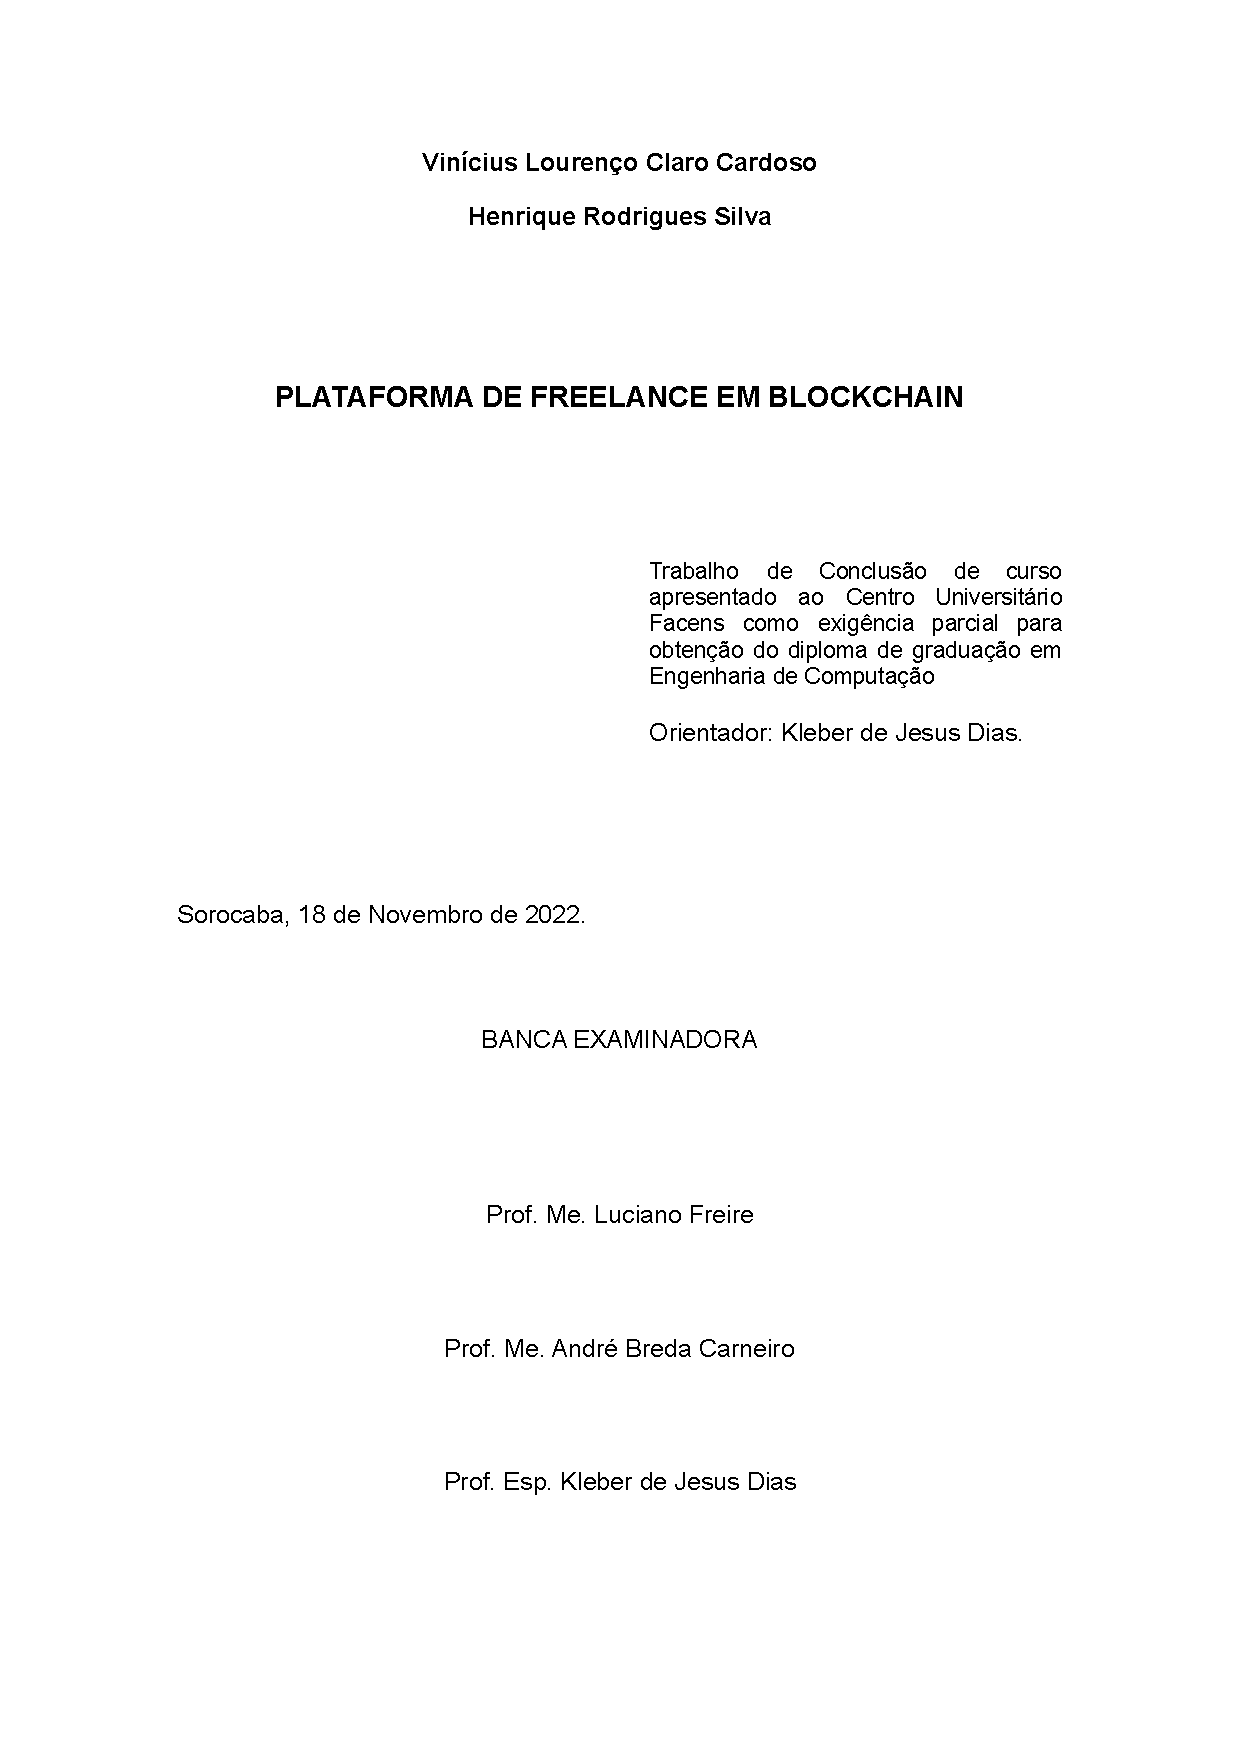
\includepdf[pages=-]{pdfs/folha_de_aprovacao.pdf}
\end{epigrafe}
% resumo em português
\setlength{\absparsep}{18pt} % ajusta o espaçamento dos parágrafos do resumo
%%\begin{resumo}
%%    Segundo a , o resumo deve ressaltar o
%%    objetivo, o método, os resultados e as conclusões do documento. A ordem e a extensão
%%    destes itens dependem do tipo de resumo (informativo ou indicativo) e do
%%    tratamento que cada item recebe no documento original. O resumo deve ser
%%    precedido da referência do documento, com exceção do resumo inserido no
%%    próprio documento. (\ldots) As palavras-chave devem figurar logo abaixo do
%%   resumo, antecedidas da expressão Palavras-chave:, separadas entre si por
%%    ponto e finalizadas também por ponto.

%%    \textbf{Palavras-chave}: latex. abntex. editoração de texto.
%%\end{resumo}

% resumo em inglês
%\begin{resumo}[Abstract]
%    \begin{otherlanguage*}{english}
%        This is the english abstract.

%        \vspace{\onelineskip}

%        \noindent 
%        \textbf{Keywords}: latex. abntex. text editoration.
%    \end{otherlanguage*}
%\end{resumo}
\input{partes/pre_textuais/lista_figuras.tex}
%\pdfbookmark[0]{\listofquadrosname}{loq}
%\listofquadros*
%\cleardoublepage
\pdfbookmark[0]{\listtablename}{lof}
\listoftables*
\cleardoublepage
\begin{siglas}
    \item[IPFS] InterPlanetary File System - Sistema de Arquivos Interplanetário
    \item[Freelancer] É um termo para descrever o profissional autónomo que realiza
serviços para outras empresas.
    \item[Workana] É uma empresa que fornece uma plataforma de Freelance.
    \item[Upwork] Assim como o Workana, é empresa que fornece uma plataforma de Freelance.
    \item[Hash] É o resultado de, ou função que, gera um mesmo resultado a partir de uma entrada de dados.
    \item[FTP] É um protocolo de transferência de arquivos entre servidor e cliente.
    \item[SMTP] É um protocolo de transmissão de e-mails.
    \item[HTTP] É um protocolo de de transferência de hiper-texto, como o HTML.
    \item[Framework] É um conjunto de ferramentas e códigos que um desenvolvedor pode utilizar para facilitar o desenvolvimento de um projeto. Os exemplos são Angular, Vue, .NET, etc.
    \item[Javascript] É a implementação da especificação ECMASCRIPT, no qual é uma linguagem não tipada e fácil de ser usada que é interpretada por todos os navegadores.
    \item[Typescript] É um super-conjunto estritamente tipado do Javascript, no qual adiciona novas funcionalidades e principalmente a tipagem a linguagem do Javascript.
    \item[Angular] É um Framework escrito em Typescript desenvolvido pela Google para desenvolvedor aplicações web.
    \item[HTML] É a sigla para HyperText Markup Language, é uma linguagem usada para definir a estrutura de uma página web.
    \item[CSS] É a sigla para Cascading Style Sheets, que é um mecanismo de aplicar estilos visuais para uma página HTML.
    \item[SCSS] É um pré-processador de CSS, que adiciona novas funcionalidades ao CSS de forma a facilitar o desenvolvimento.
\end{siglas}
\input{partes/pre_textuais/sumario.tex}

% ----------------------------------------------------------
% ELEMENTOS TEXTUAIS
% ----------------------------------------------------------
\textual % informa o inicio da numeração de páginas em algarismos arábicos
\chapter{Introdução}
% ----------------------------------------------------------

Em 2008, \citeauthor{bitcoin} descreveu em um trabalho chamado de \textit{Bitcoin: A Peer-to-Peer Eletronic Cash System} uma maneira de realizar pagamentos digitais, ao utilizar criptomoedas, de forma descentralizada. Isso significa que para realizar a transferência de um valor para outra pessoa, não é necessário que exista uma instituição financeira para validar que quem está transferindo realmente possui o valor, a própria rede do \textit{Bitcoin} garantirá essa validação, resolvendo assim o problema do gasto-duplo.

A tecnologia principal que move esse sistema de pagamento é o \textit{Blockchain}, uma maneira de armazenar dados de forma extremamente segura que funciona como uma lista de blocos que são interligados uns aos outros de forma a garantir que os dados registrados nos blocos sejam imutáveis.\cite{blockchain}

A partir dessa tecnologia, em 2014, Vitalik Buterin publicou um trabalho para apresentar o \textit{Ethereum}, um protocolo que roda com a tecnologia de Blockchain e permite criar aplicações decentralizadas através de \textit{Smart Contracts}. \cite{ethereum_yellow} O \textit{Smart Contract} é uma forma de escrever um contrato que pode ser executado de forma automática.\cite{smart_contract} \cite{smart_contract_blockchain}

Com essas tecnologias, em 2022, é possível realizar pagamentos entre pessoas de qualquer parte do mundo sem que ninguém possa impedir, e também ter a posse digital de uma obra de arte onde tem-se uma prova imutável de que você é o dono dela. Em um mundo onde tudo está cada vez mais conectado, a necessidade de ter sistemas distribuídos está se mostrando uma peça fundamental para a liberdade individual, de forma que, você possa comprar ou ter algo sem que ninguém possa censurar ou retirar de você.\cite{decentralization}

Contudo, ainda é necessário que você possua dinheiro no mundo digital para que você possa realizar pagamentos e compras, e uma das formas de ganhar dinheiro é através de \textit{Freelance}, onde você realiza algum trabalho e recebe por esse trabalho. Ao pensar sobre as soluções existentes hoje, existe o Workana e o Upwork mas são plataformas que tem toda a sua estrutura centralizada e não realizam pagamentos em criptomoeda.

Com isso, o problema que esse trabalho se propõe a resolver é a criação de uma plataforma de \textit{Freelance} totalmente descentralizada, de forma que, você possa postar projetos, ser contratado e ganhar pelos trabalhos realizados em criptomoedas. Além disso, com um sistema de resolução de conflitos, a ideia é dar mais segurança aos \textit{Freelancers} e contratantes para entrarem e continuarem na plataforma.

% DEV: Removido porque o sistema de pontuação não foi feito até o momento, se acabarmos fazendo, adicionar esse trecho novamente.
% Além disso, com um sistema de resolução de conflitos e outro para pontuação, a ideia é incentivar bons \textit{Freelancers} a entrarem e continuarem na plataforma.

% DEV: Mesmo problema do anterior, removido porque não há o sistema 
% Essa plataforma tem como o objetivo de ser simples de ser usada, totalmente descentralizada com sistema de pontuação para premiar e evidenciar bons \textit{Freelancers}. 
Além disso, ao ser totalmente descentralizado, ela se diferenciará de outras plataformas de \textit{Freelance} em \textit{Blockchain} que possuem alguns dos seus sistemas centralizados em troca de melhorar a usabilidade.

Um ponto importante de uma plataforma de \textit{Freelance} é a resolução de conflitos e quando será feito os pagamentos, visto que, é possível que haja pessoas má intencionadas querendo roubar o dinheiro de um contratante, ou mesmo, o contratante não querendo pagar o \textit{Freelance}, esses dois problemas serão descritos nos próximos capítulos.

Para construir a plataforma, será utilizado principalmente \textit{Smart Contracts}, que rodará em uma rede de \textit{Blockchain} chamada \textit{Polygon}, uma alternativa para a \textit{Ethereum} que possui taxas de transações muito mais baixas, além de processar as transações mais rapidamente. E assim como na \textit{Ethereum}, que possui a moeda principal \textit{ether}, na \textit{Polygon} temos o Matic, que será usado para realizar o pagamento das taxas das transações.\cite{polygon}

Além dos \textit{Smart Contracts}, será criado um site que posteriormente será disponibilizado aos usuários através do protocolo \textit{IPFS}, que é um sistema de armazenamento permanente de arquivos de forma descentralizada. Uma vez que os arquivos estejam no sistema do \textit{IPFS}, para ser excluído, todos na rede que possuem uma cópia precisam ativamente excluir essa cópia.\cite{ipfs}

Para esse trabalho, é esperado no final dele a criação dos contratos inteligentes, assim como, um site para servir de interface para os contratos que estarão disponibilizados em uma rede de \textit{Blockchain} e no protocolo \textit{IPFS}. Contudo, esse trabalho não irá abranger a comunicação entre duas pessoas de forma descentralizada e anônima, a comunicação ainda será responsabilidade do contratante e do \textit{Freelancer}.

Este trabalho está organizado da seguinte maneira: no Capítulo 2 será feito uma revisão teórica sobre os conceitos apresentados na introdução para explicar sobre a descentralização e como é feita a segurança de todo o sistema. No Capítulo 3, será apresentado as tecnologias e serviços utilizados para a criação da plataforma. No Capítulo 4, será mostrado detalhes da implementação da plataforma, além de mostrar o design dos \textit{Smart Contracts} e da estrutura do site construído. No capítulo 5, será feito uma análise do que foi desenvolvido, assim como, discutir ideias de possíveis melhorias para futuros trabalhos. Por fim, no Capítulo 6, será feito a conclusão que discutirá os objetivos e os conhecimentos que foram obtidos e aprofundados durante todo o projeto.

\include{abntex2-modelo-include-comandos}

\chapter{Referencial teórico}\label{cap_trabalho_academico}

Como mencionado no capítulo anterior, a criação da plataforma é baseado em diversas tecnologias e conceitos que asseguram a segurança de um sistema descentralizado.

Dessa forma, nesse capítulo será abordado os pontos essenciais para entender a criação do projeto, tais como: o que é um Freelancer e uma plataforma de Freelance, sistemas centralizados e descentralizados, \textit{Ethereum} e redes similares, a importância do \textit{Bitcoin} como um sistema de pagamento, entre outros tópicos.

\section{Contexto}

Antes de entrar em conceitos fundamentais, é necessário entender sobre o que se trata o projeto, ou seja, entender o que é um Freelancer, o que são plataformas de Freelance e quais são as plataformas que existem hoje.

\subsection{Freelancer}

\textit{Freelancers} são pessoas autônomas que têm uma associação de curto prazo baseada em tarefas com o empregador e, não são empregados da empresa. A sua associação com a empresa é apenas até que a tarefa atribuída seja concluída com sucesso.\cite{freelance}

Eles tem a obrigação de completar a tarefa com alta qualidade dentro do prazo acordado em troca de dinheiro (previamente acordado com o empregador). Durante o tempo que o freelancer estiver realizando a tarefa, ele fica livre para realizar acordo com diversos empregadores, resumindo, os \textit{freelancers} realizam vários projetos em paralelo.

\subsection{Plataformas de Freelance}
Plataformas \textit{freelancer} têm mantido perfis de trabalho dos \textit{freelancers} e empregadores para ajuda-los a estabelecer confiança mútua, servindo como uma ponte de ligação entre os dois perfis. Além disso, os empregadores depositam o valor do serviço do freelance para a plataforma, que só libera o valor para o freelance depois da entrega do serviço ser validada pelo empregador.\cite{freelance}

À medida que a cultura de \textit{freelancer} ficou famosa durante todos esses anos, centenas de sites foram lançados que fornecem serviços \textit{freelancer}. Entre os mais famosos da internet podemos citar \textit{Upwork}, \textit{People Per Hour} e \textit{Fiverr} e no Brasil, \textit{Workana} \cite{the_freelancer}.

\subsubsection{Workana}

\textit{Workana} é uma plataforma de mercado para trabalho \textit{freelancer} e remoto, de contratação de trabalhadores independentes. A empresa tem sua sede na Argentina e possui escritórios no Brasil, na Colômbia e no México, a plataforma está disponível em espanhol, inglês e português. \cite{workana}

Ao usar o \textit{Workana} como empregador você pode: publicar um projeto para começar a receber propostas, pode interagir e selecionar o melhor \textit{freelancer}, e por fim, realizar o pagamento do trabalho realizado para o \textit{freelancer}. E como \textit{freelancer}, você pode encontrar projetos, enviar propostas para os clientes e trabalhar com total autonomia. \cite{workana}

\subsubsection{Upwork}

\textit{Upwork}, anteriormente \textit{Elance-oDesk}, é uma plataforma americana de \textit{freelancers} atualmente com sede em Santa Clara e São Francisco, Califórnia. Em 2017, \textit{Upwork} tinha mais de 12 milhões de \textit{freelancers} registrados e 5 milhões de clientes. Em março de 2022, a \textit{Upwork} foi nomeada para a lista das 100 empresas mais influentes do ano de 2022 da \textit{TIME}. \cite{upwork}

Assim como a \textit{Workana}, é possível criar projetos, selecionar \textit{freelancers}, realizar pagamentos do trabalhos contratados e receber por esses trabalhos realizados como \textit{freelancer}.

\section{Conceitos Fundamentais}

Abaixo, será falado um pouco dos conceitos fundamentais que irá ser o pilar das tecnologias e ferramentas apresentadas posteriormente no trabalho. E partir desses conceitos, será possível entender como a \textit{Blockchain} e \textit{Bitcoin} funcionam, dessa forma, entender também o por que dessas tecnologias terem sido escolhidas para desenvolver a plataforma.

\subsection{Sistemas Centralizados}

Um sistema centralizado pode ser descrito como uma arquitetura de cliente e servidor, no qual o cliente realiza requisições e o servidor responde as requisições recebidas de um cliente. E esse sistema, no começo da Word Wide Web, se tornou muito popular através dos protocolos como: \textit{File Transfer Protocol} (FTP), \textit{Simple Mail Transfer Protocol} (SMTP)
e \textit{Hypertext Transfer Protocol} (HTTP). \cite{client_server_model}

\begin{figure}[h!]
  \centering
  \caption{Arquitetura Cliente/Servidor}
  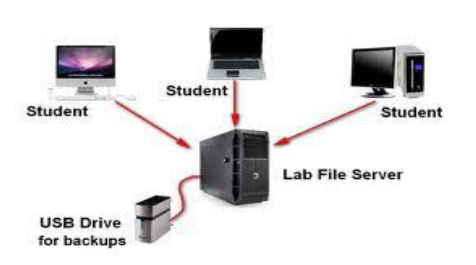
\includegraphics[width=300px]{src/images/client-server.png}
  \subcaption{Fonte: \cite{client_server_model} }
  \label{fig:client_server_fig}
\end{figure}

Para \citeauthor{held2000server}, um computador, notebook ou dispositivo é representação de um cliente, e junto de um servidor, possuem uma relação de cooperação para executar uma ação iniciada pelo cliente final que retornará algum recurso ou modificará algum estado dentro do servidor. A representação dos diversos clientes conectando em um único servidor é descrito na Figura \ref{fig:client_server_fig}.

\subsection{Sistemas Descentralizados}

De acordo com \cite{distributed}, um sistema descentralizado, ou um sistema distribuído, é a composição de diversos computadores que forma um sistema que se comunica em uma rede de computadores, de forma que, através de protocolos como \textit{HTTP}, \textit{SMTP}, etc... permitem a execução de atividades de forma distribuída.

\cite[p.17]{design_distributed_systems} diz que "devido à sua natureza distribuída, quando estruturados adequadamente, os sistemas distribuídos são inerentemente mais confiáveis". Diferente do modelo de cliente-servidor, a mesma tarefa pode ser executada em diversos computadores, de forma que, se ocorrer uma falha em computador, o sistema ainda continua operando por que a tarefa pode ser processada por qualquer computador conectado no sistema.

Além da confiabilidade e da disponibilidade, em um âmbito mais amplo, \citeauthor{decentralization} descreve que a descentralização pode ser usada para construir uma estrutura de governança que permita diversos grupos viverem de forma pacífica. Isso ocorre porque uma estrutura descentralizada não é baseada em confiança em uma autoridade central, ao contrário disso, ela delega poder a autoridades menores para ter mais efetividade e segurança ao não ter um ponto central de falha.

\section{Tecnologias}

Nesta seção, será falado sobre as tecnologias que compõem a plataforma e porque elas foram construídas, de forma que, exemplifique a sua importância na criação da plataforma.

\subsection{Blockchain}

O \textit{Blockchain} é uma tecnologia para armazenar as informações de forma segura e imutável através do que ela chama de blocos. Os blocos são um recipiente onde é agrupado diversas transações e, após uma certa quantidade de transações, um bloco é finalizado e outro bloco é criado, ao mesmo tempo, uma assinatura digital chamado de \textit{Hash} é criado associando o bloco anterior com o novo bloco, como pode ser visto na Figura \ref{fig:blockchain_structure} \cite{blockchain}.

\begin{figure}[h!]
  \centering
  \caption{Representação da estrutura do Blockchain.}
  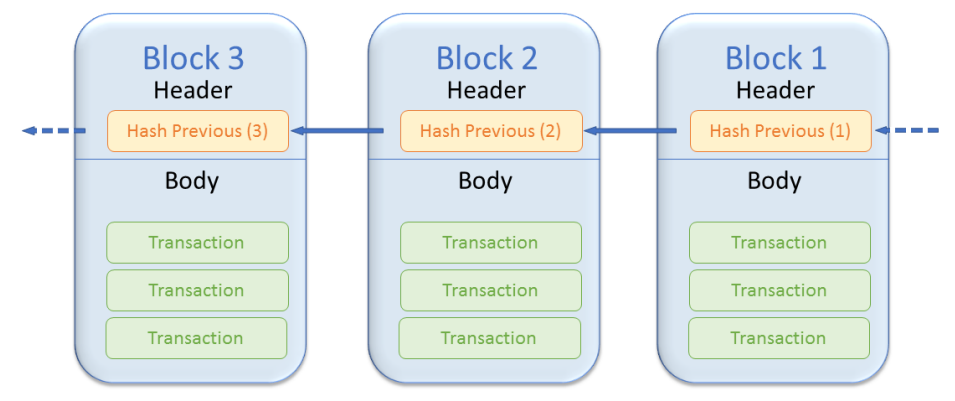
\includegraphics[width=300px]{src/images/representacao_blocos_blockchain.png}
  \subcaption{Fonte: \cite{blockchain_ref_for_block_explanation}}
  \label{fig:blockchain_structure}
\end{figure}

Ao associar um bloco ao anterior, se um participante malicioso deseja alterar o conteúdo de um bloco passado, ele necessariamente irá alterar o \textit{Hash} desse mesmo bloco, porque o \textit{Hash} é gerado baseado no conteúdo do bloco. Ao modificar o \textit{Hash}, qualquer bloco que foi gerado posteriormente, e que estava conectado a esse bloco modificado, se tornará inválido. Isso acontece por que os blocos posteriores não vão possuir o novo \textit{Hash}, e dessa forma, para detectar um bloco modificado só seria necessário comparar o \textit{Hash} do bloco atual e o \textit{Hash} no bloco posterior \cite{blockchain_ref_for_block_explanation}. 

Dessa forma, ao usar a estrutura do \textit{Blockchain}, é possível criar uma rede onde qualquer pessoa pode participar ao possuir uma cópia do histórico de transações, reduzindo a necessidade de confiança entre as partes e aumentando a transparência ao permitir que qualquer pessoa possa auditar as transações armazenadas \cite{blockchain}.

Contudo, para coordenar todos os participantes da rede, é necessário que haja algum algoritmo de consenso de forma a suportar as falhas bizantinas, que é quando a falha de um nó faz com que o sistema como um todo fique comprometido \cite{byzantine_fault_tolerance}. Na seção a seguir, será explicado os algoritmos de consenso e também como o \textit{Bitcoin} propôs uma solução para esse problema.

\subsection{Bitcoin}

Segundo \cite{bitcoin2}, \textit{Bitcoin} é um sistema descentralizado de dinheiro eletrônico \textit{Peer-to-Peer} (P2P) sem um servidor central ou partes confiáveis. Os usuários têm as chaves criptográficas para o seu próprio dinheiro e transacionam diretamente na rede com outros usuários do sistema.

Em poucas palavras, o \textit{Bitcoin} é uma forma de dinheiro, assim como o real, o dólar ou o euro, com a diferença de ser puramente digital e não ser emitido por nenhum governo. O seu valor é determinado livremente pelos indivíduos no mercado. Para transações online, é a forma ideal de pagamento, pois é rápido, barato e seguro.

Além disso, para resolver o problema de gasto-duplo, assim como as falhas de Bizantino, o \textit{Bitcoin} utiliza o algoritmo de consenso chamado \textit{Proof-of-Work} (Prova de Trabalho). A ideia inicial desse tipo de técnica para solucionar o problema foi introduzido por \cite{pricing_via_processing}, onde descrito uma função que necessitasse de um custo computacional relevante para escrever uma mensagem, ao mesmo tempo em que, fosse barato para verificar se essa mensagem era verdadeira.

E alguns anos mais tarde, \cite{proofs_of_work_original} trouxe a ideia do protocolo chamado de \textit{Proof-of-Work}, ou prova de trabalho. \citeauthor{proofs_of_work_original} o descrevia como "um protocolo no qual um provador demonstra a um verificador que ele gastou um certo nível de esforço computacional em um intervalo de tempo especificado". 

Dessa forma, \citeauthor{bitcoin} utilizou esse protocolo e o montou da seguinte maneira: é necessário que o bloco submetido na rede possua uma prova de trabalho, isso garante que, para fraudar a rede, seja necessário ter mais de 51\% do poder computacional porque só dessa forma seria possível ultrapassar a velocidade de outros nós e convencer que a sua versão é a correta. Além disso, a dificuldade dessa prova de trabalho é constantemente reajustada, com o objetivo de manter um tempo médio de criação de um novo bloco em torno de 10 minutos, isso ajuda a evitar que um novo modelo de computador quebre o equilíbrio da rede.

\subsection{Ethereum}

Assim como o \textit{Bitcoin}, o \textit{Ethereum} é um sistema descentralizado de dinheiro eletrônico e também pode ser descrito por \cite{ethereum2}, como uma rede de criptomoedas popular que pode suportar DApps.

No começo do desenvolvimento do trabalho, a \textit{Ethereum} possuía um modelo de consentimento baseado em \textit{Proof-of-Work}, contudo, ouve uma migração para o tipo de consentimento chamado \textit{Proof-of-Stake} com o objetivo de diminuir as taxas de transação e o consumo de energia.

A ideia por trás do \textit{Proof-of-Stake} é fornecer proteção contra o ataque de fraude ao possuir 51\% da rede, além de permitir uma capacidade maior de transações por segundo e também reduzir custos de taxa de transação. Como \cite{larimer2013transactions} descreve, a ideia é ter nós responsáveis por dizer se um bloco é válido ou não, e em essência, toda rede é em partes um \textit{Proof-of-Stake} porque há nós com direito de decidir se um bloco é válido ou não. 

Contudo, na \textit{Ethereum}, o que dá esse direito é o depósito que o dono do nó faz antecipadamente. Esse depósito tem o objetivo de garantir e assegurar que o dono do nó não vá querer cometer alguma fraude, e caso uma fraude venha a ocorrer por aquele nó, o dinheiro depositado é totalmente perdido. Porém, ao utilizar esse tipo de consenso, a segurança como um todo é diminuída porque é necessário a coordenação de menos nós para que ocorra uma fraude na rede. 

\subsection{Peer-to-Peer}

\textit{Peer-to-Peer} refere-se a troca direta de algum ativo, como uma moeda digital, entre partes individuais sem o envolvimento de uma autoridade central. Uma troca de moeda estritamente \textit{peer-to-peer} foi o principal objetivo que impulsionou a criação do \textit{Bitcoin}. \cite{peer-to-peer}

\subsection{Smart Contracts}

\textit{Smart Contracts}, traduzido como Contratos Inteligentes, são scripts auto-executáveis que residem em \textit{blockchain}, tem como objetivo permitir adequação, distribuição e automatização de fluxos de trabalho. \cite{smart_contract2}

É definida por \citeauthor{smart_contract} como “um protocolo de transação computadorizado que executa os termos de um contrato". Os contratos inteligentes nos permitem que cálculos de propósito geral ocorram na cadeia. No entanto, eles se destacam quando são encarregados de gerenciar interações orientadas por dados entre entidades da rede.

\subsection{DApps}

Um aplicativo descentralizado (\textit{DApp}) é um aplicativo construído em uma rede descentralizada que combina um contrato inteligente e uma interface de usuário front-end sendo executado em uma rede \textit{Peer-to-Peer}. No \textit{Ethereum}, os contratos inteligentes são acessíveis e transparentes – como \textit{APIs} abertas – para que seu \textit{DApp} possa até incluir um contrato inteligente que outra pessoa tenha escrito.\cite{DApps}

\section{Resolução de Conflitos}

Nesta seção, será falado sobre os aspectos da resolução de conflitos, uma vez que as duas partes podem ter um desacordo um com o outro, como a plataforma lidará para resolver esse conflito. Para chegar em uma solução, será descrito primeiro o que será considerado um conflito e quais as formas que a academia encontrou de resolver, e qual é a forma que foi escolhida.

\subsection{Definição de conflito}

Para \cite[p.18]{rahim2017managing}, o conflito é "um processo interativo manifestado em incompatibilidade, desacordo ou dissonância dentro ou entre entidades sociais". Ao aplicar o contexto de uma interação entre duas pessoas no qual uma deseja contratar a outra, um conflito pode surgir quando, por exemplo, a parte contratante acha que o que foi entregue não é suficiente e o contratado acredita que deve receber pelo serviço prestado.

Já \cite{nicholson1992rationality} define que é uma atividade entre seres conscientes, que não necessariamente são racionais, além disso, é necessário ter termos, necessidades ou obrigações entre as partes envolvidas. Ao estender, (\citeauthor{nicholson1992rationality}) também completa que um conflito pode existir quando duas pessoas querem realizar ações que são mutuamente incompatíveis.

Para ambos os autores, o que define o conflito é o desacordo e as ações mutuamente incompatíveis, e alinhado ao exemplo do contrante e o contratado, temos que um conflito é algo comum e que precisa ser tomado ações pacíficas entre ambas as partes para ser resolvido, e é sobre isso que tratará a próxima seção.

\subsection{Formas de Resolução de Conflito}

Em seu livro, \cite{bercovitch2019social} menciona três formas básicas de resolução de conflito:

\begin{itemize}
\item Com coerção ou violência.
\item Com negociação ou barganha.
\item Ou com uma intervenção de um terceiro.
\end{itemize}

Se tratando de uma sociedade onde violência é inaceitável, a primeira opção está fora de cogitação para a plataforma porque o intuito é fornecer segurança e confiabilidade aos usuários da plataforma.

Sobre a negociação, \cite[p.3]{behavioral_theory_of_labor_negotations} sugeria que negociação era "uma interação deliberada de duas ou mais unidades sociais complexas que estão tentando definir ou redefinir os termos de sua interdependência". Quanto a barganha, \cite{nicholson1992rationality} descrevia a barganha como um conflito parcial de objetivos no qual as partes se esforçam para encontrar um acordo mutuamente satisfatório. Dessa forma, a plataforma em si não precisa fazer nada proativamente em busca de resolver esse conflito, visto que, tanto na negociação quanto na barganha, é necessário apenas o envolvimento das partes interessadas e que o conflito não seja completamente irreconciliável.

Contudo, em um caso onde o conflito chegue ao ponto de ser irreconciliável, é possível optar para a terceira forma de resolução de conflito, a intervenção de um terceiro, no qual será falado em mais detalhes na próxima seção.

\subsection{Intervenção de Terceiros}

Quando se faz necessário a intervenção de um terceiro para a resolução de um conflito, o que antes era uma díade acaba se tornando uma tríade, e dessa forma, esse terceiro agente tem o poder de afetar os resultados e o comportamentos das partes envolvidas \cite{bercovitch2019social}.

Além disso, \citeauthor{bercovitch2019social} diz que esse tipo de resolução de conflito ocorre quando o conflito se estende por muito tempo ou é muito complexo, as partes encontram um ponto onde não há como prosseguir e quando a continuação do conflito é um fator de cansaço para ambas as partes.

Quando aplicado o contexto da plataforma, podemos ter que um contratante queira que o projeto venha em uma qualidade maior, e ao mesmo tempo, o contratado deseja receber pelo trabalho feito. Quando as negociações não ocorrerem, a plataforma irá confiar a resolução desse conflito a um terceiro.

Além disso, o \cite[p.13]{bercovitch2019social} menciona que "a base do envolvimento de terceiros é voluntária", dessa forma, a plataforma irá oferecer uma solução para ambas as partes apontarem um terceiro que terá a responsabilidade de validar os fatos e decidir quem está certo nesse conflito.

Para incentivar a resolução de conflito em todas as partes envolvidas, o sistema de publicação de projeto, até o sistema de se candidatar a um projeto seguirá as seguintes regras:

\begin{itemize}
\item O contratante precisa depositar o pagamento de forma integral na plataforma.
\item O contratado precisa depositar uma porcentagem do pagamento que irá receber.
\item Caso ocorra a intervenção de um terceiro, ele terá direito a ficar com uma porcentagem sobre o valor total a ser pago entre as partes.
\end{itemize}

Nesse cenário, tanto o contratante quanto o contratado possuem interesse em resolver o conflito para que o dinheiro depositado seja estornado, e no caso do contrante, que o projeto que ele pediu seja entregue. Ao mesmo tempo, é criado um incentivo financeiro até mesmo para a existência de um mercado para vender serviços de resolução de conflito de forma profissional.

\section{Trabalhos Correlatos}

Ao criar esse projeto, foi importante também entender quais os trabalhos que foram desenvolvidos até o presente momento. Para começar, \cite{gandhi2019decentralized} propôs uma solução descentralizada, baseada em \textit{Ethereum} e \textit{IPFS}, no qual possui dois contratos que tem a responsabilidade de lidar com usuários e lidar com as propostas publicadas por cada usuário. 

Diferente deste trabalho, \citeauthor{gandhi2019decentralized} optaram por utilizar a  rede principal do \textit{Ethereum}, essa opção pode ter sido levada em conta porque o preço do Ethereum, em 2019, estava entorno dos 200 \textit{USD} \cite{ethereum_price_2019} e a taxa de transação era baixa, e em 2022, esse preço passa dos 2,800 \textit{USD} \cite{ethereum_price_2022} e as taxas são caras demais para simples transações.

Em uma solução similar, \cite{freelancing_blockchain_related} constroem uma plataforma de freelance utilizando o \textit{Ethereum}, e diferente de \citeauthor{gandhi2019decentralized}, eles não hospedam a aplicação dentro do \textit{IPFS}, o que faz com que seja necessário confiar em um servidor centralizado para armazenar a interface de comunicação dos contratos na \textit{Blockchain}.

Contudo, é importante notar que em ambos os trabalhos não há uma menção ou sugestão sobre como lidar com conflitos de uma entrega, e nem incentivos ou garantias, seja por parte do contratado quanto do contratante, de fornecerem bons projetos e boas ofertas de trabalho, porque não há um custo real para fazer essas ofertas. Assim sendo, este trabalho se diferencia ao propor uma solução para esse problema, além de entregar garantias e seguranças que uma tecnologia descentralizada como a do \texit{Blockchain} proporciona.



\chapter{Desenvolvimento}

Nesta seção, será falado mais sobre os aspectos que envolveram toda a fase de desenvolvimento, explicando um pouco da arquitetura do software, passando para explicação do site, depois será falado sobre \textit{Smart Contracts} e terminará com a explicação de como foi feito os testes de todo o código produzido.

\section{Arquitetura}

Para um sistema de plataforma de Freelance, é possível imaginar diversas arquiteturas complexas com diversos componentes e serviços. Cada sistema tem seus requisitos e os desenvolvedores que participam da construção desse software são os principais responsáveis por definirem como será feito.

Para a plataforma de freelance, foi escolhido uma arquitetura mais simples, fácil de ser apresentada e de manter, além disso, que permite todo o sistema evoluir no futuro caso seja necessário.

Na figura \ref{fig:architecture_fig} pode-se ver como funcionará um fluxo básico de criação de projeto, onde o usuário interage com a camada do site que está em \textit{IPFS}, acessa o site, cria um projeto e depois passa por mais algumas camadas até que a informação do projeto seja escrita em \textit{Blockchain}.

\begin{figure}[h!]
  \centering
  \caption{Fluxo de um Usuário}
  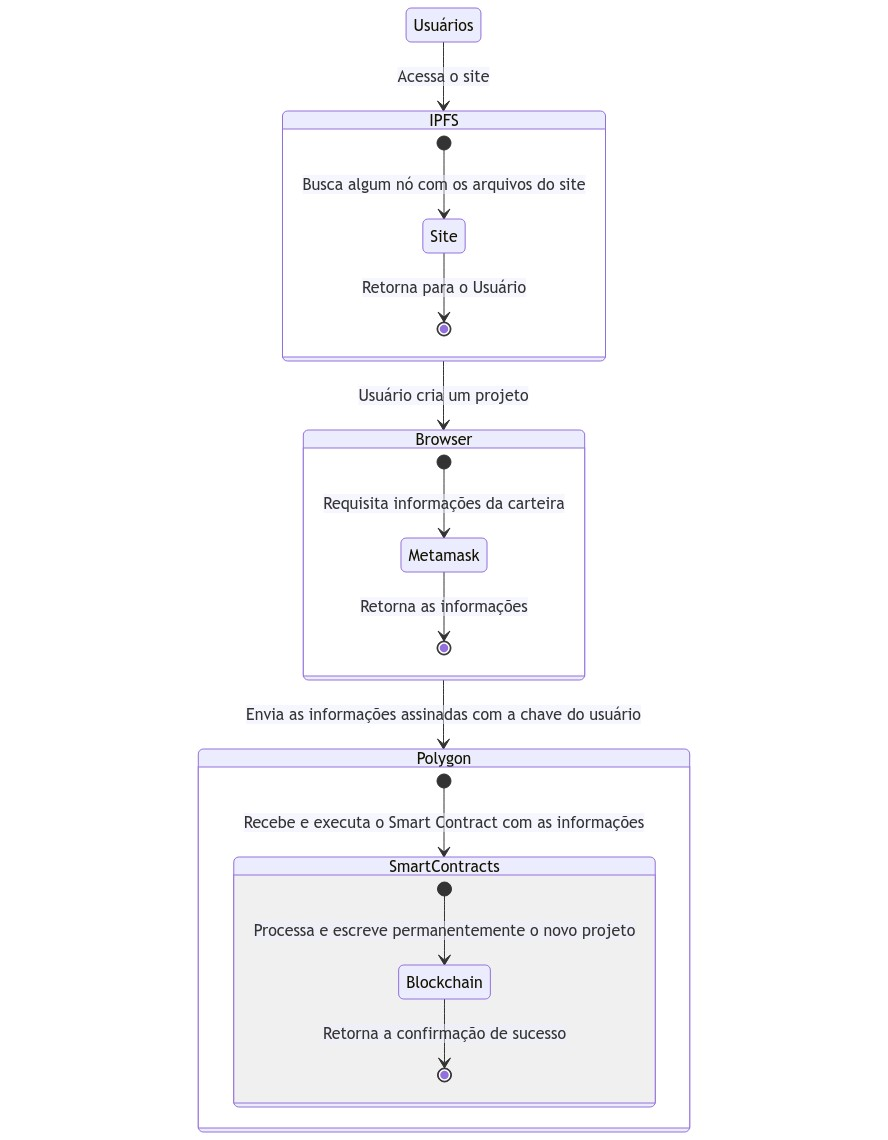
\includegraphics[width=300px]{src/images/architecture.jpeg}
  \subcaption{Fonte: Autor }
  \label{fig:architecture_fig}
\end{figure}

Seria possível construir uma \textit{API} - Interface de Programação de Aplicação - para ser responsável por fazer a comunicação com o \textit{Blockchain}, mas para garantir um sistema que seja resiliente, foi optado por manter a comunicação entre o usuário e a \textit{Blockchain} de forma direta. 

O uso de uma \textit{API} nesses casos tem como finalidade melhorar a UX porque pode ser colocado camadas de cache que melhoram o tempo de acesso a informação, contudo, faz com que esses pontos acabem sendo centralizados, o que foge do escopo dos objetivos propostos.

Portanto, será desenvolvido o site que ficará hospedado dentro da rede \textit{IPFS}, no qual o usuário poderá acessar a qualquer momento, e ele irá interagir com o site usando o \textit{Metamask} que guardará as chaves da conta do usuário na rede \textit{Polygon}.

O \textit{Metamask} será o responsável por assinar qualquer requisição para a \textit{Polygon}. Dessa forma, ao criar um projeto, é assinado a mensagem com as informações, e depois é enviado do navegador para o \textit{Polygon} que irá executar e armazenar os resultados da transação do \textit{Smart Contract}.

\section{Site}

% * Adicionar referências *

O site, com nome de Freedapp, foi desenvolvido em \textit{Angular} 13, que é um \textit{framework} - plataforma de aplicação - mantido pela \textit{Google}, baseado em código aberto e escrito em \textit{Typescript}, linguagem de programação que é um superconjunto sintático estrito de \textit{Javascript}, outra linguagem de programação de alto nível principalmente utilizada na \textit{web}.

A principal razão para se utilizar o \textit{Angular} é sua facilidade e sua organização estrutural, simplificando o processo de desenvolvimento e a estrutura de código desenvolvido. O \textit{framework} possui uma clara divisão entre a camada de exibição(visual) e a de regra de negócios(lógica).

Dentro da estrutura do \textit{Angular}, é utilizado \textit{HTML}, \textit{SCSS} e \textit{Typescript} para criação de aplicações web. O \textit{HTML} é utilizado para criar a estrutura de elementos de uma página. O \textit{SCSS} são códigos de estilo para customizar a estrutura da página baseado em \textit{CSS}. Combinando o \texti{HTML} e o \textit{SCSS}, é possível montar a estrutura e estilizar a página para que fique fácil e agradável de usar. 

Além da estrutura estética da página é necessário haver lógica para execução das funcionalidades e regras de negócio, para isso, usa-se o \textit{Typescript}, criando uma interação entre o usuário e o código do sistema. O \textit{Typescript} pode ser usado para definir ações como: ao clicar em um botão, faça uma chamada para a \textit{Blockchain} e execute o contrato, por exemplo, \textit{CriarProposta}.

Em adição as vantagens citadas acima sobre o \textit{Angular}, é muito importante a escolha de um \textit{Framework} que fosse \textit{SPA - Single Page Application} (Aplicação de Página Única) no qual toda a interação e navegação é feita apenas em uma única página. O \texti{SPA} permite a criação de uma aplicação de formar fácil e interativa, produzindo no final apenas um único arquivo \textit{HTML} e diversos outros arquivos dependentes do \texti{HTML} que possibilitam a interpretação do navegador sem a necessidade de um servidor dinâmico.

Depois de desenvolvido todo o site, o FreedApp será hospedado dentro do \textit{IPFS}, para esse projeto, foi escolhido o serviço chamado \textit{NFT Storage}, onde é possível subir qualquer arquivos sem a necessidade de pagar nada. Após hospedar, para visualizar a página \textit{HTML}, será usado a \textit{Cloudflare}, uma empresa com serviços em nuvem que disponibiliza gratuitamente um serviço que se conecta com o \textit{IPFS} e disponibiliza os arquivos armazenados na rede de uma forma muito mais rápida e com cache global.

Antes de começar o desenvolvimento do FreedApp foi desenvolvido um protótipo navegável (layout) no \textit{Figma}, um editor gráfico de prototipagem de projetos. Facilitando a visualização do projeto e criação das regras de negócio e fluxo de informações sem a necessidade de criação de códigos e retrabalho posterior.

Com as estruturas e tecnologias citadas acima, começa-se o desenvolvimento das páginas, da navegação e das funcionalidades do site. Para facilitar a navegação do usuário dentro do site, foi criado um menu lateral com as principais funcionalidades da aplicação, elas são, em resumo: 

\begin{itemize}
\item Início, é uma página com diversas propostas diferentes, as quais, podem interessar o usuário que está utilizando o sistema
\item Lances, em lances o usuário logado pode verificar os seus nas propostas que teve interesse
\item Propostas, o empregador pode criar propostas para seus projetos e publica-las para buscar por lances e a ajuda dos freelancers
\item Disputas, é a página onde são resolvidos os conflitos das propostas. Existem algumas etapas para conclusão dos conflitos, consistindo em escolher um mediador, escolher a distribuição e depois realizar o pagamento de acordo com a distribuição.
\item Ajuda, serve para tirar as dúvidas e mostrar tutoriais ao usuário para utilização do sistema, do \textit{Metamask} entre outras.
\end{itemize}

\section{Smart Contracts}

Para a criação dos \textit{Smart Contracts} será utilizado a linguagem de programação \textit{Solidity} em conjunto com bibliotecas como \textit{ethers} e \textit{Open Zeppelin}, que fornecem as funcionalidades de conexão com os contratos e abstração de funcionalidades básicas de contratos, respectivamente.

Ao desenvolver um contrato, é necessário tomar cuidados como: a quantidade de operações executadas, o tamanho do contrato e problemas de segurança. A seguir, será discutido um pouco mais em detalhes como será tratado cada um desses problemas.

A quantidade de operações executadas é um problema, porque dentro do \textit{Solidity}, cada operação, como salvar o estado de uma variável ou ler esse estado, custa um certo valor de poder computacional chamado \textit{Gas}. A soma dessas operações terá um custo chamado \textit{Gas}, que será repassado para quem executar a transação, dessa forma, é interessante que o menor número de operações possíveis seja chamada para realizar a ação que o usuário deseja.

Para lidar com quantidade de operações executadas, os contratos serão organizados da seguinte forma: em vez de armazenar os projetos em uma estrutura como uma lista, será usado o que é chamado de \textit{mapping}, uma estrutura no \textit{Solidity} onde funciona como uma espécie de \textit{Tabela de Hash}. Ao se usar essa estrutura em conjunto com uma variável para contar a quantidade de itens armazenados, é possível economizar bastante \textit{Gas} porque ambas as operações de contar e pegar o projeto possuirá uma complexidade de tempo \textit{O(1)}.

O problema do tamanho do contrato é uma limitação da \textit{Blockchain}, porque o tamanho do contrato precisa ser menor que 24KiB, para evitar que contratos enormes tornassem a rede de \textit{Blockchain} lenta.

Dessa forma, as funcionalidades da plataforma será dividida em três contratos: Proposta, Lances e Disputa. Ao dividir as funcionalidades em mais de um contrato, será possível manter-se abaixo do tamanho limite ao mesmo tempo em que divide responsabilidades e simplifica o código.

Por fim, quando se trata de lidar com dinheiro, a segurança é imprescindível. Um problema de segurança muito conhecido é chamado de \textit{Reentrancy}, onde um código que transfere um dinheiro para uma carteira pode ser manipulado para que esse mesmo trecho de código seja executado diversas vezes, até que o contrato original fique sem dinheiro algum.

Para mitigar esse problema, é necessário que haja uma validação para fazer com que antes de transferir o dinheiro, essa transferência só ocorra uma única vez. Um exemplo de como fazer isso, é verificar se o usuário tem dinheiro na conta, e depois zerar o dinheiro do usuário e só ai realizar a transferência. Nesse ultimo caso, mesmo que ocorra o problema de \textit{Reentrancy}, não será transferido dinheiro algum.

\section{Testes}

É fundamental em qualquer código escrito que haja algum tipo de teste para assegurar que o comportamento esperado realmente se concretize. Quando se trata de testes, os mais comuns são testes unitários e testes de integração.

O propósito do teste unitário é testar uma função única, como por exemplo checar se o resultado de uma função com uma certa entrada de dados sempre retornará o mesmo valor. Ao usar dependências externas, é necessário realizar um \textit{mock}, que basicamente simula um valor para garantir uma certa imutabilidade no teste para testar apenas a entrada.

E quanto ao teste de integração, ele é utilizado para testar uma funcionalidade praticamente que por completo, entrando no contexto da \textit{Blockchain}, seria como rodar um nó e rodar um \textit{Smart Contract} e ver os valores sendo salvos na \textit{Blockchain}.

Para esse projeto, será criado testes de integração para todos os \textit{Smart Contracts} criados com uma cobertura de 100\%, com o objetivo de garantir uma maior confiabilidade nas funcionalidades criadas. 

Com os testes, será possível começar a rodar e testar os contratos sem necessariamente depender de finalizar o site, o que garante uma agilidade e uma paralelização do desenvolvimento do projeto. 

%Este modelo vem com o ambiente \texttt{quadro} e impressão de Lista de quadros 
%configurados por padrão. Verifique um exemplo de utilização:

%\begin{quadro}[htb]
%    \caption{\label{quadro_exemplo}Exemplo de quadro}
%    \begin{tabular}{|c|c|c|c|}
        %\hline
        %\textbf{Pessoa} & \textbf{Idade} & \textbf{Peso} & \textbf{Altura} \\ %\hline
%        Marcos & 26    & 68   & 178    \\ \hline
%        Ivone  & 22    & 57   & 162    \\ \hline
%        ...    & ...   & ...  & ...    \\ \hline
%        Sueli  & 40    & 65   & 153    \\ \hline
%    \end{tabular}
%    \fonte{Autor.}
%\end{quadro}

%Este parágrafo apresenta como referenciar o quadro no texto, requisito
%obrigatório da ABNT. 
%Primeira opção, utilizando \texttt{autoref}: Ver o \autoref{quadro_exemplo}. 
%Segunda opção, utilizando  \texttt{ref}: Ver o Quadro \ref{quadro_exemplo}.
% ---
% primeiro capitulo de Resultados
% ---
\chapter{Resultados}
% ---

A seguir, será apresentado o resultado do que foi produzido do desenvolvimento do site e dos \textit{Smart Contracts}.

\section{Site}

% * Usar mais o nome do APP "Freedapp" *

Conforme previsto nos objetivos, o site foi desenvolvido e hospedado dentro da rede IPFS com o \textit{CID} igual a \textit{bafybeifhmnl4pgzuuyvujv3w57zfb3tftejo3ksjtiubh3fajvu65uk5li}, e pode ser encontrado no link \href{https://cloudflare-ipfs.com/ipfs/bafybeifhmnl4pgzuuyvujv3w57zfb3tftejo3ksjtiubh3fajvu65uk5li/}{https://cloudflare-ipfs.com/ipfs}.

A página de início, figura \ref{fig:home_page_fig}, é a primeira a ser exibida ao entrar no site, é a principal página da aplicação. Todas as proposta cadastradas no sistemas estão nessa página em forma de \textit{cards} com informação resumidas das propostas, como nome do projeto e o status da proposta.

\begin{figure}[h!]
  \centering
  \caption{Tela de início}
  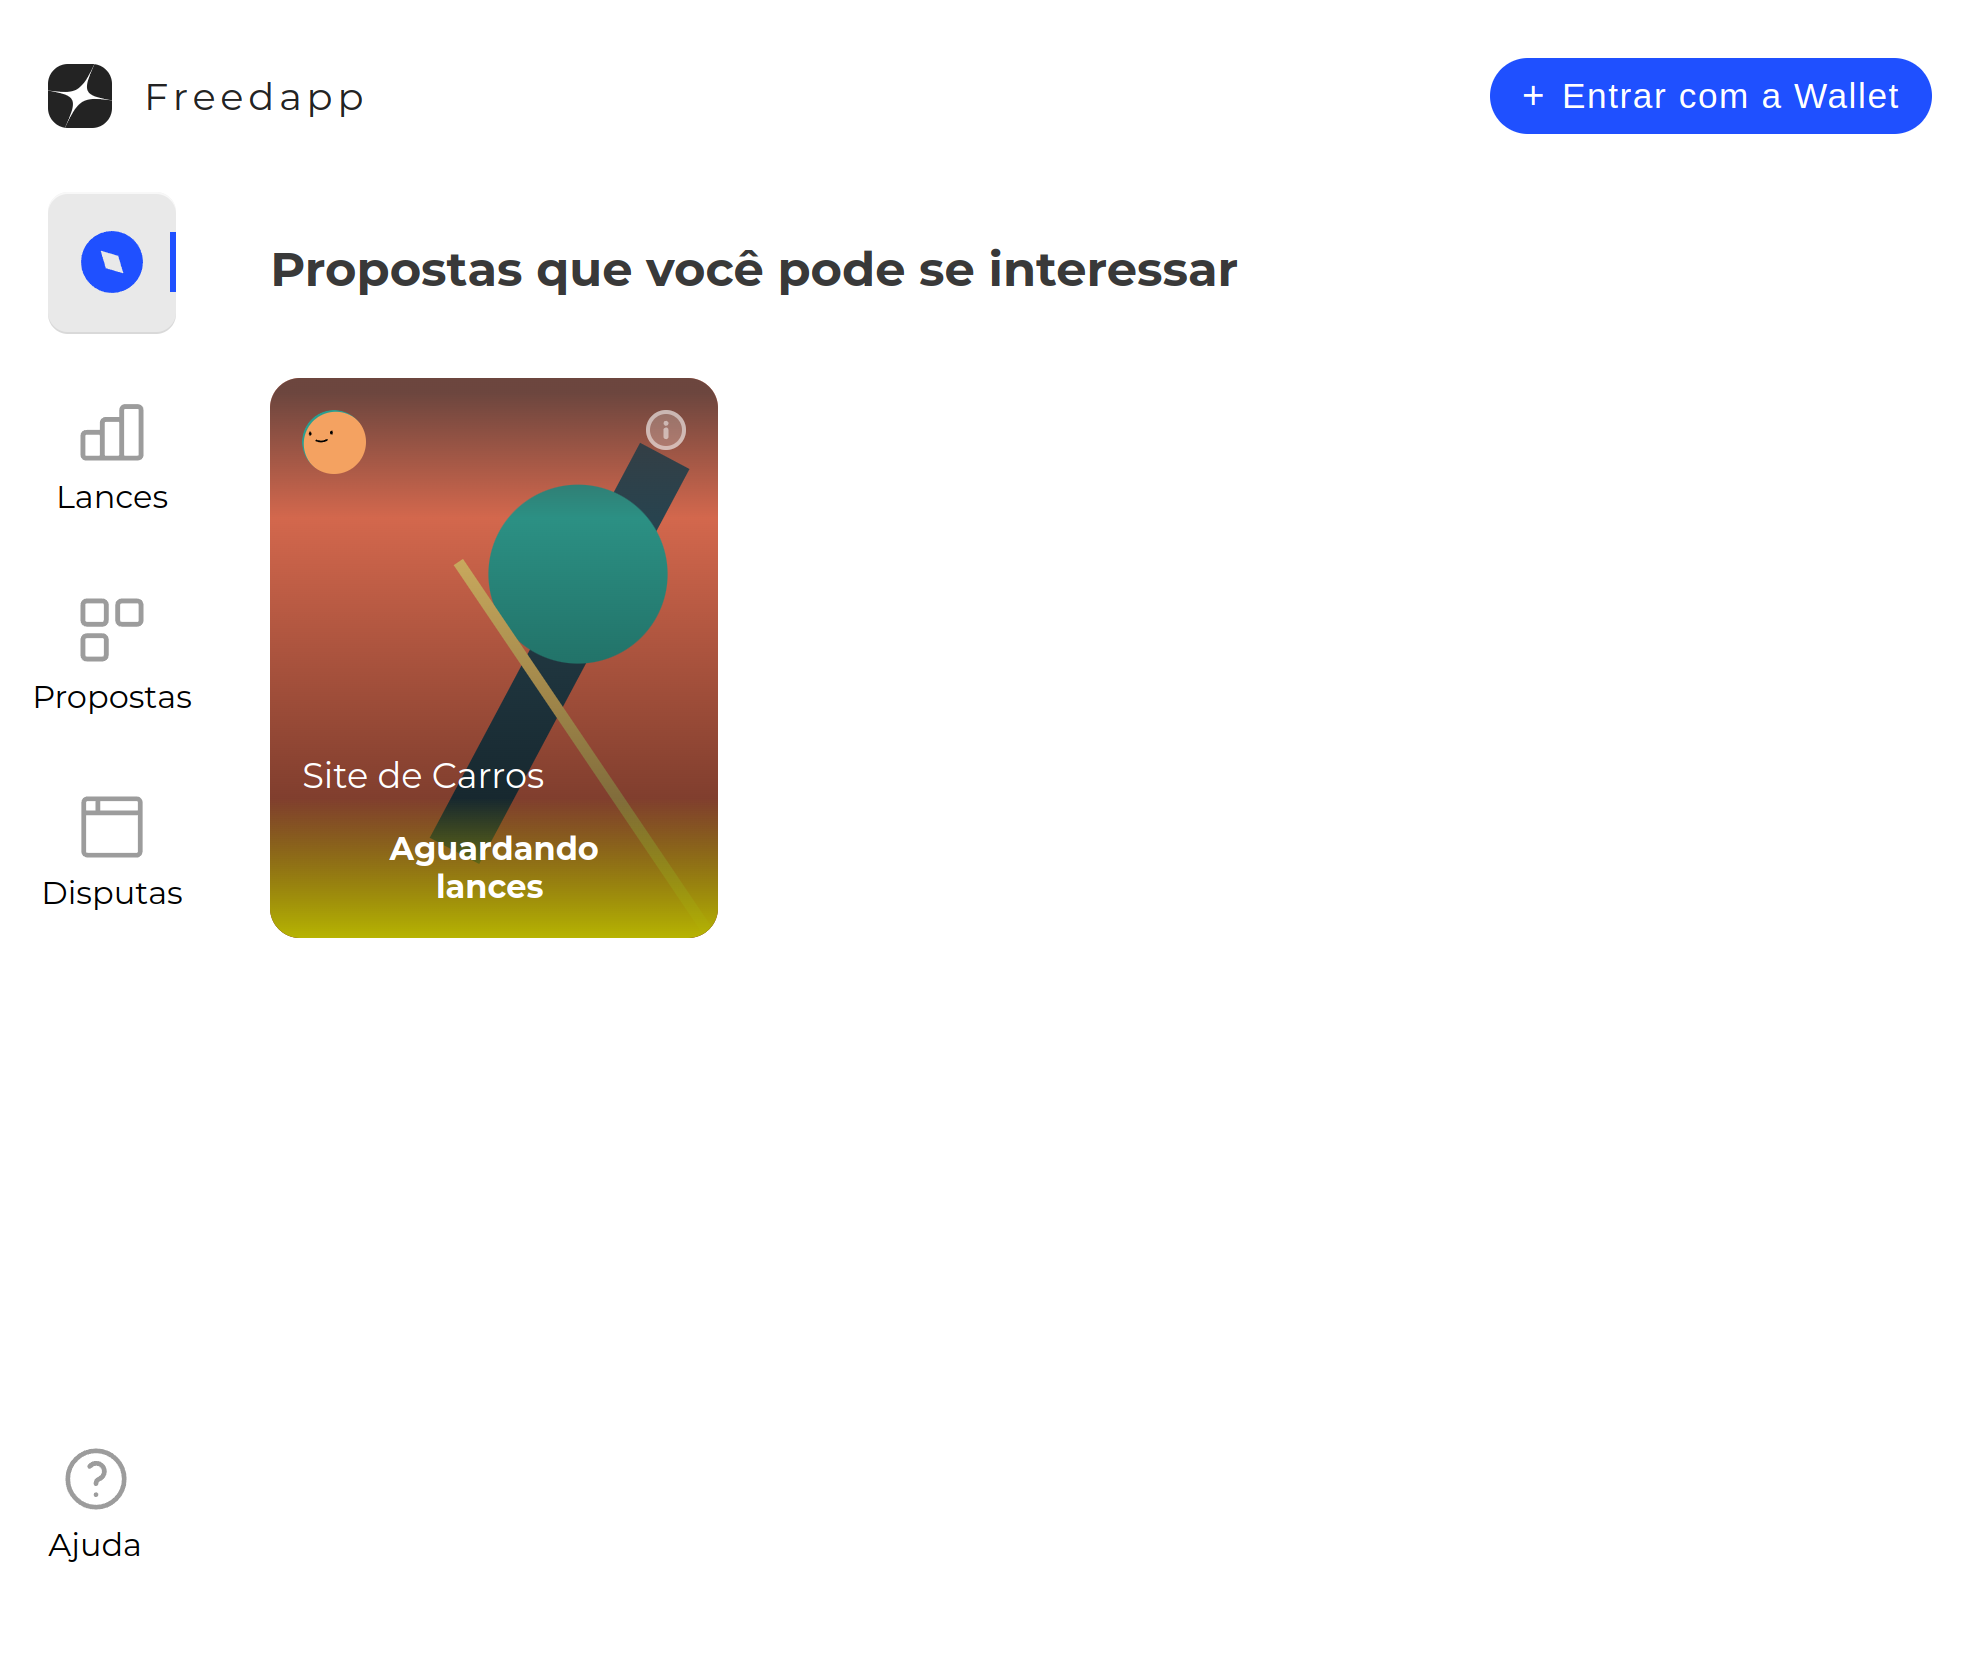
\includegraphics[width=450px]{src/images/app/home_page.png}
  \subcaption{Fonte: Autor }
  \label{fig:home_page_fig}
\end{figure}

Pode-se clicar nos itens da lista, redirecionando o usuário para uma página mais detalhada sobre a proposta. Além de, no canto da página, poder entrar com sua \textit{wallet} e conectar-se ao \textit{Metamask} para utilizar o \textit{Ethereum} como moeda para suas transações.

Em mais detalhes da proposta (figura \ref{fig:proposal_detail_page_state_waiting_bid_fig}), pode-se visualizar mais informações sobre a proposta. Ver seu nome, sua descrição, seu valor, a identificação do criador, a lista de lances que a proposta já recebeu com valor do lance, identificação do criador do lance e data de criação do lance e também a opção do usuário, caso queira, dar seu próprio lance na proposta. Além disso, pode-se visualizar o botão de ''Cancelar proposta'' caso você seja o criador daquela proposta.

\begin{figure}[h!]
  \centering
  \caption{Tela de detalhes de uma proposta}
  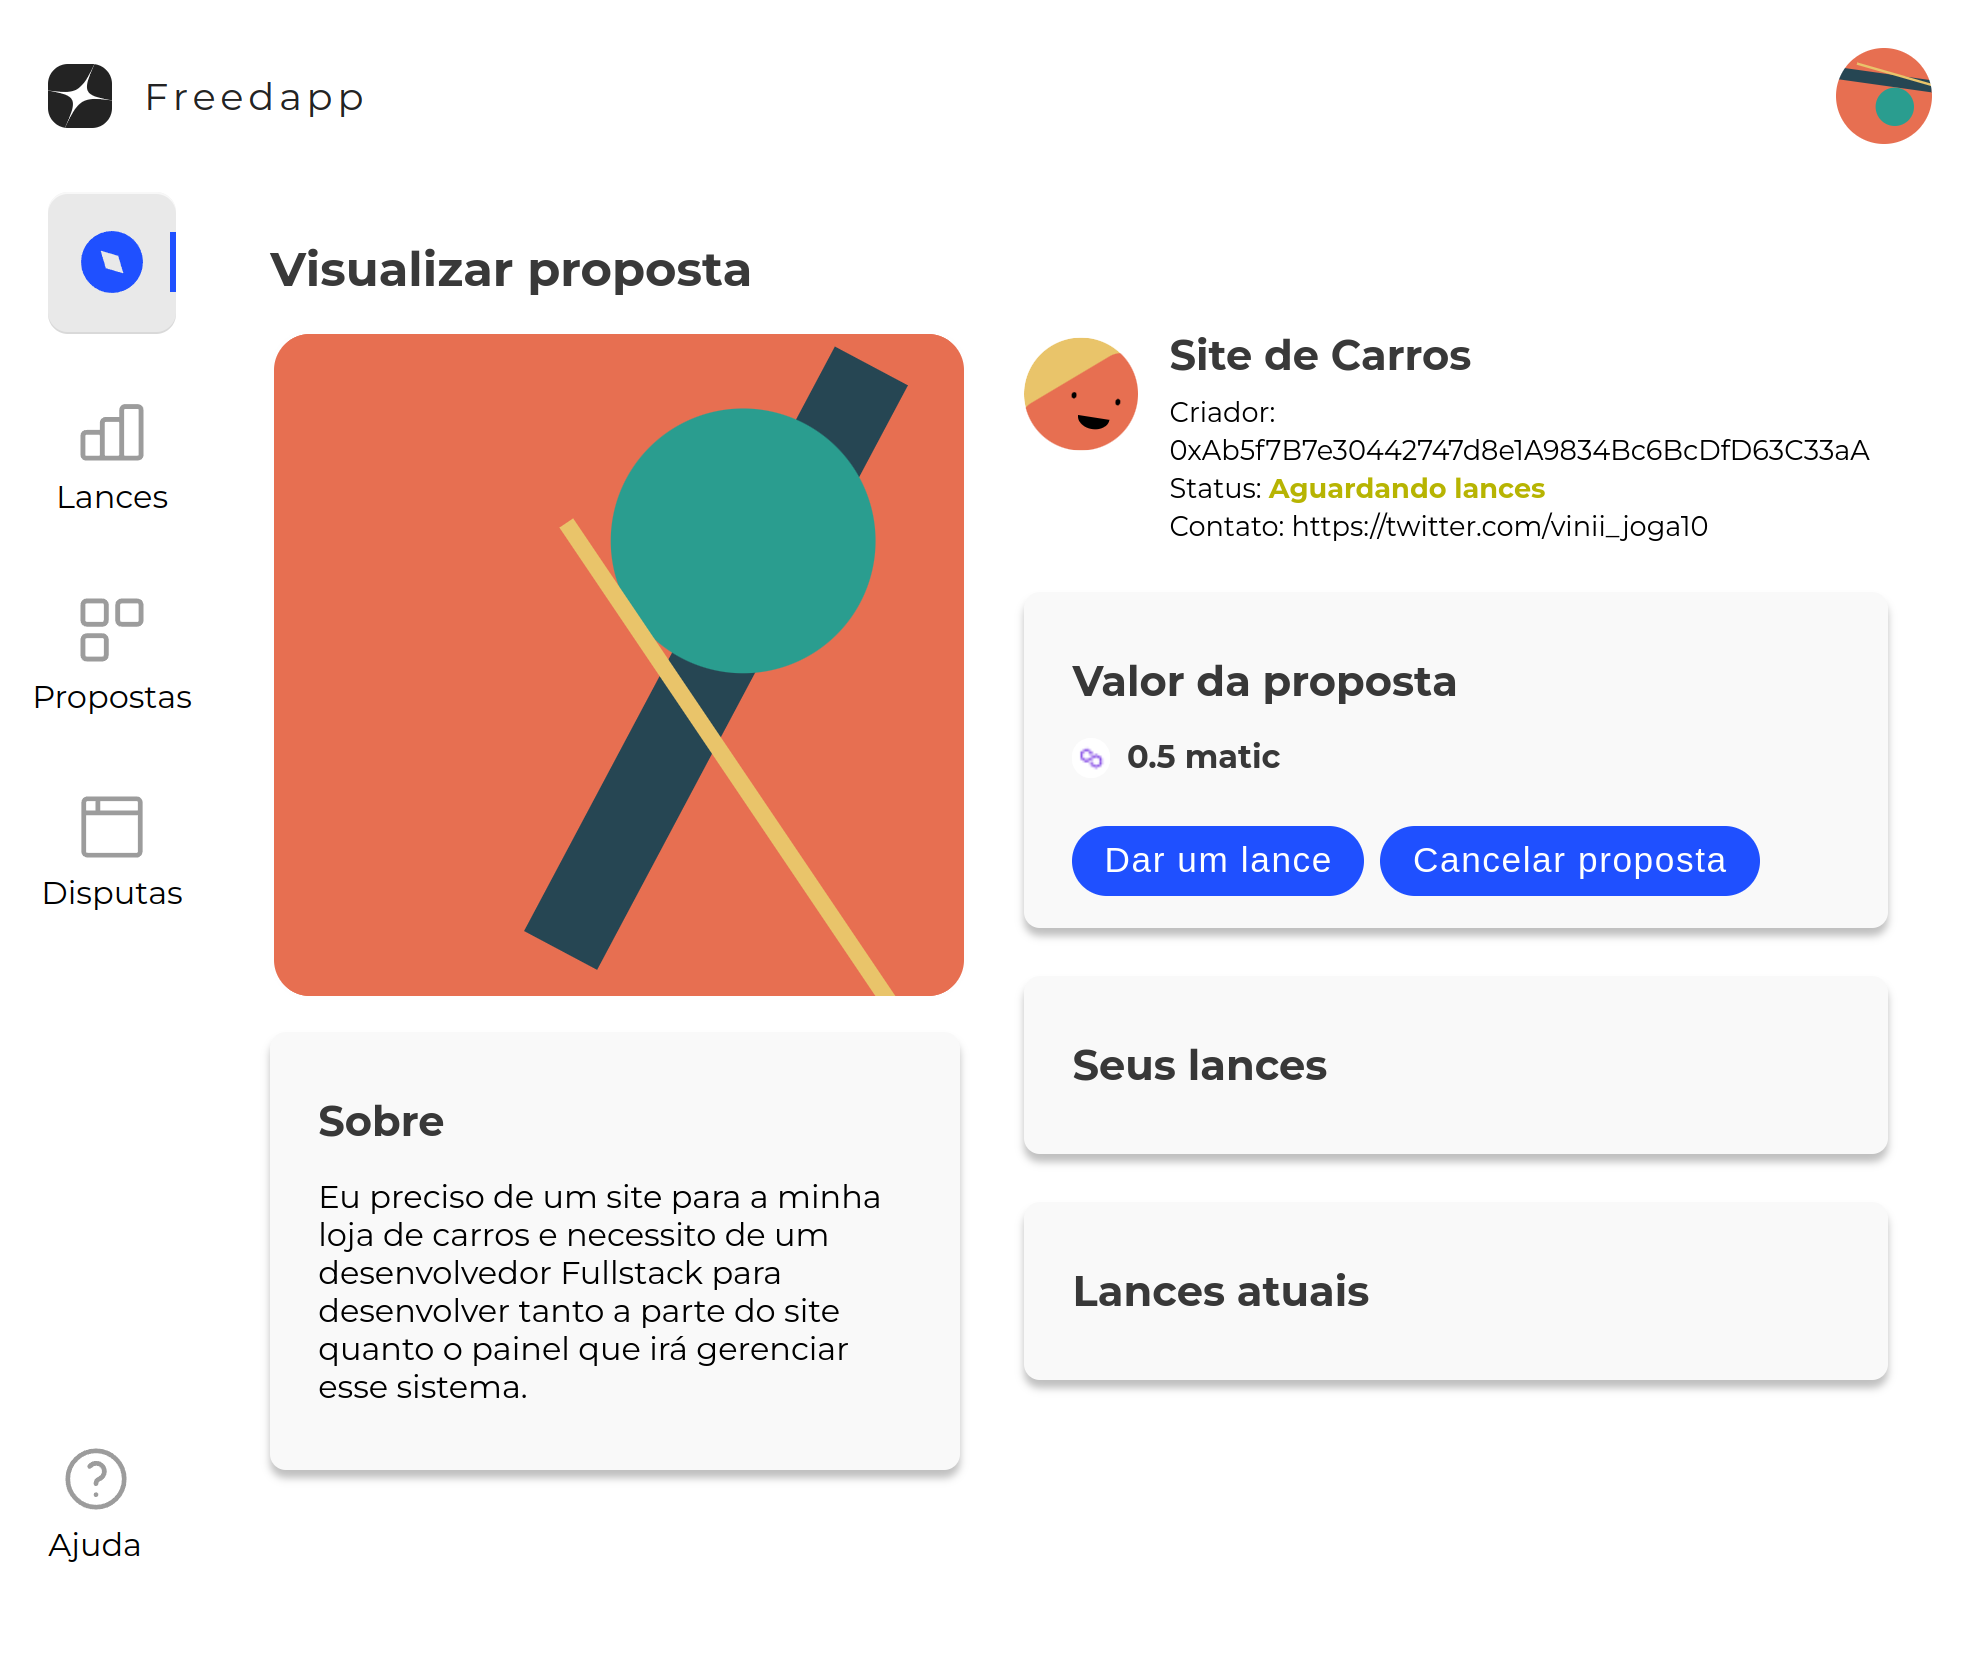
\includegraphics[width=450px]{src/images/app/proposal_detail_page_state_waiting_bid.png}
  \subcaption{Fonte: Autor }
  \label{fig:proposal_detail_page_state_waiting_bid_fig}
\end{figure}

Ao clicar em ''Dar um lance'' (figura \ref{fig:create_bid_modal_approval_fig}), é aberto automaticamente um popup do \textit{Metamask} para aprovar o lance sobre aquela proposta. O valor do lance é 5\% do valor da proposta, no qual é usado para filtrar pessoas realmente interessadas na proposta, e esse valor pode ser restituído se o usuário decidir cancelar o lance.

\clearpage

\begin{figure}[!h]
  \centering
  \caption{Modal do Metamask para aprovar a criação do lance}
  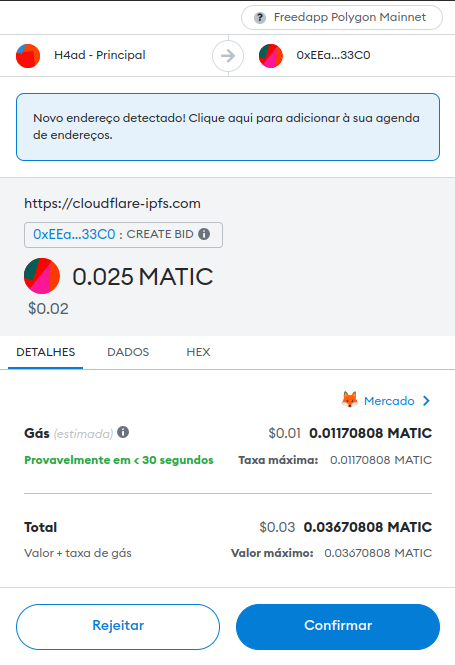
\includegraphics[height=450px]{src/images/app/create_bid_modal_approval.png}
  \subcaption{Fonte: Autor }
  \label{fig:create_bid_modal_approval_fig}
\end{figure}

Assim, ao confirmar, um novo componente gráfico aparecerá na tela (figura \ref{fig:proposal_detail_see_bid_fig}), caso o lance seja do usuário logado, irá ficar separado como "Seu lance", na qual, existe a possibilidade de visualizar a informação do seu lance ou remover o lance. Caso o lance não seja do usuário em questão, aparece como um item a mais na lista de lances daquela proposta. Ao retirar seu lance da proposta feito anteriormente, ele não pode ser mais selecionado pelo criador da proposta.

\clearpage

\begin{figure}[!h]
  \centering
  \caption{Visualizar um lance criado em aguardando lances}
  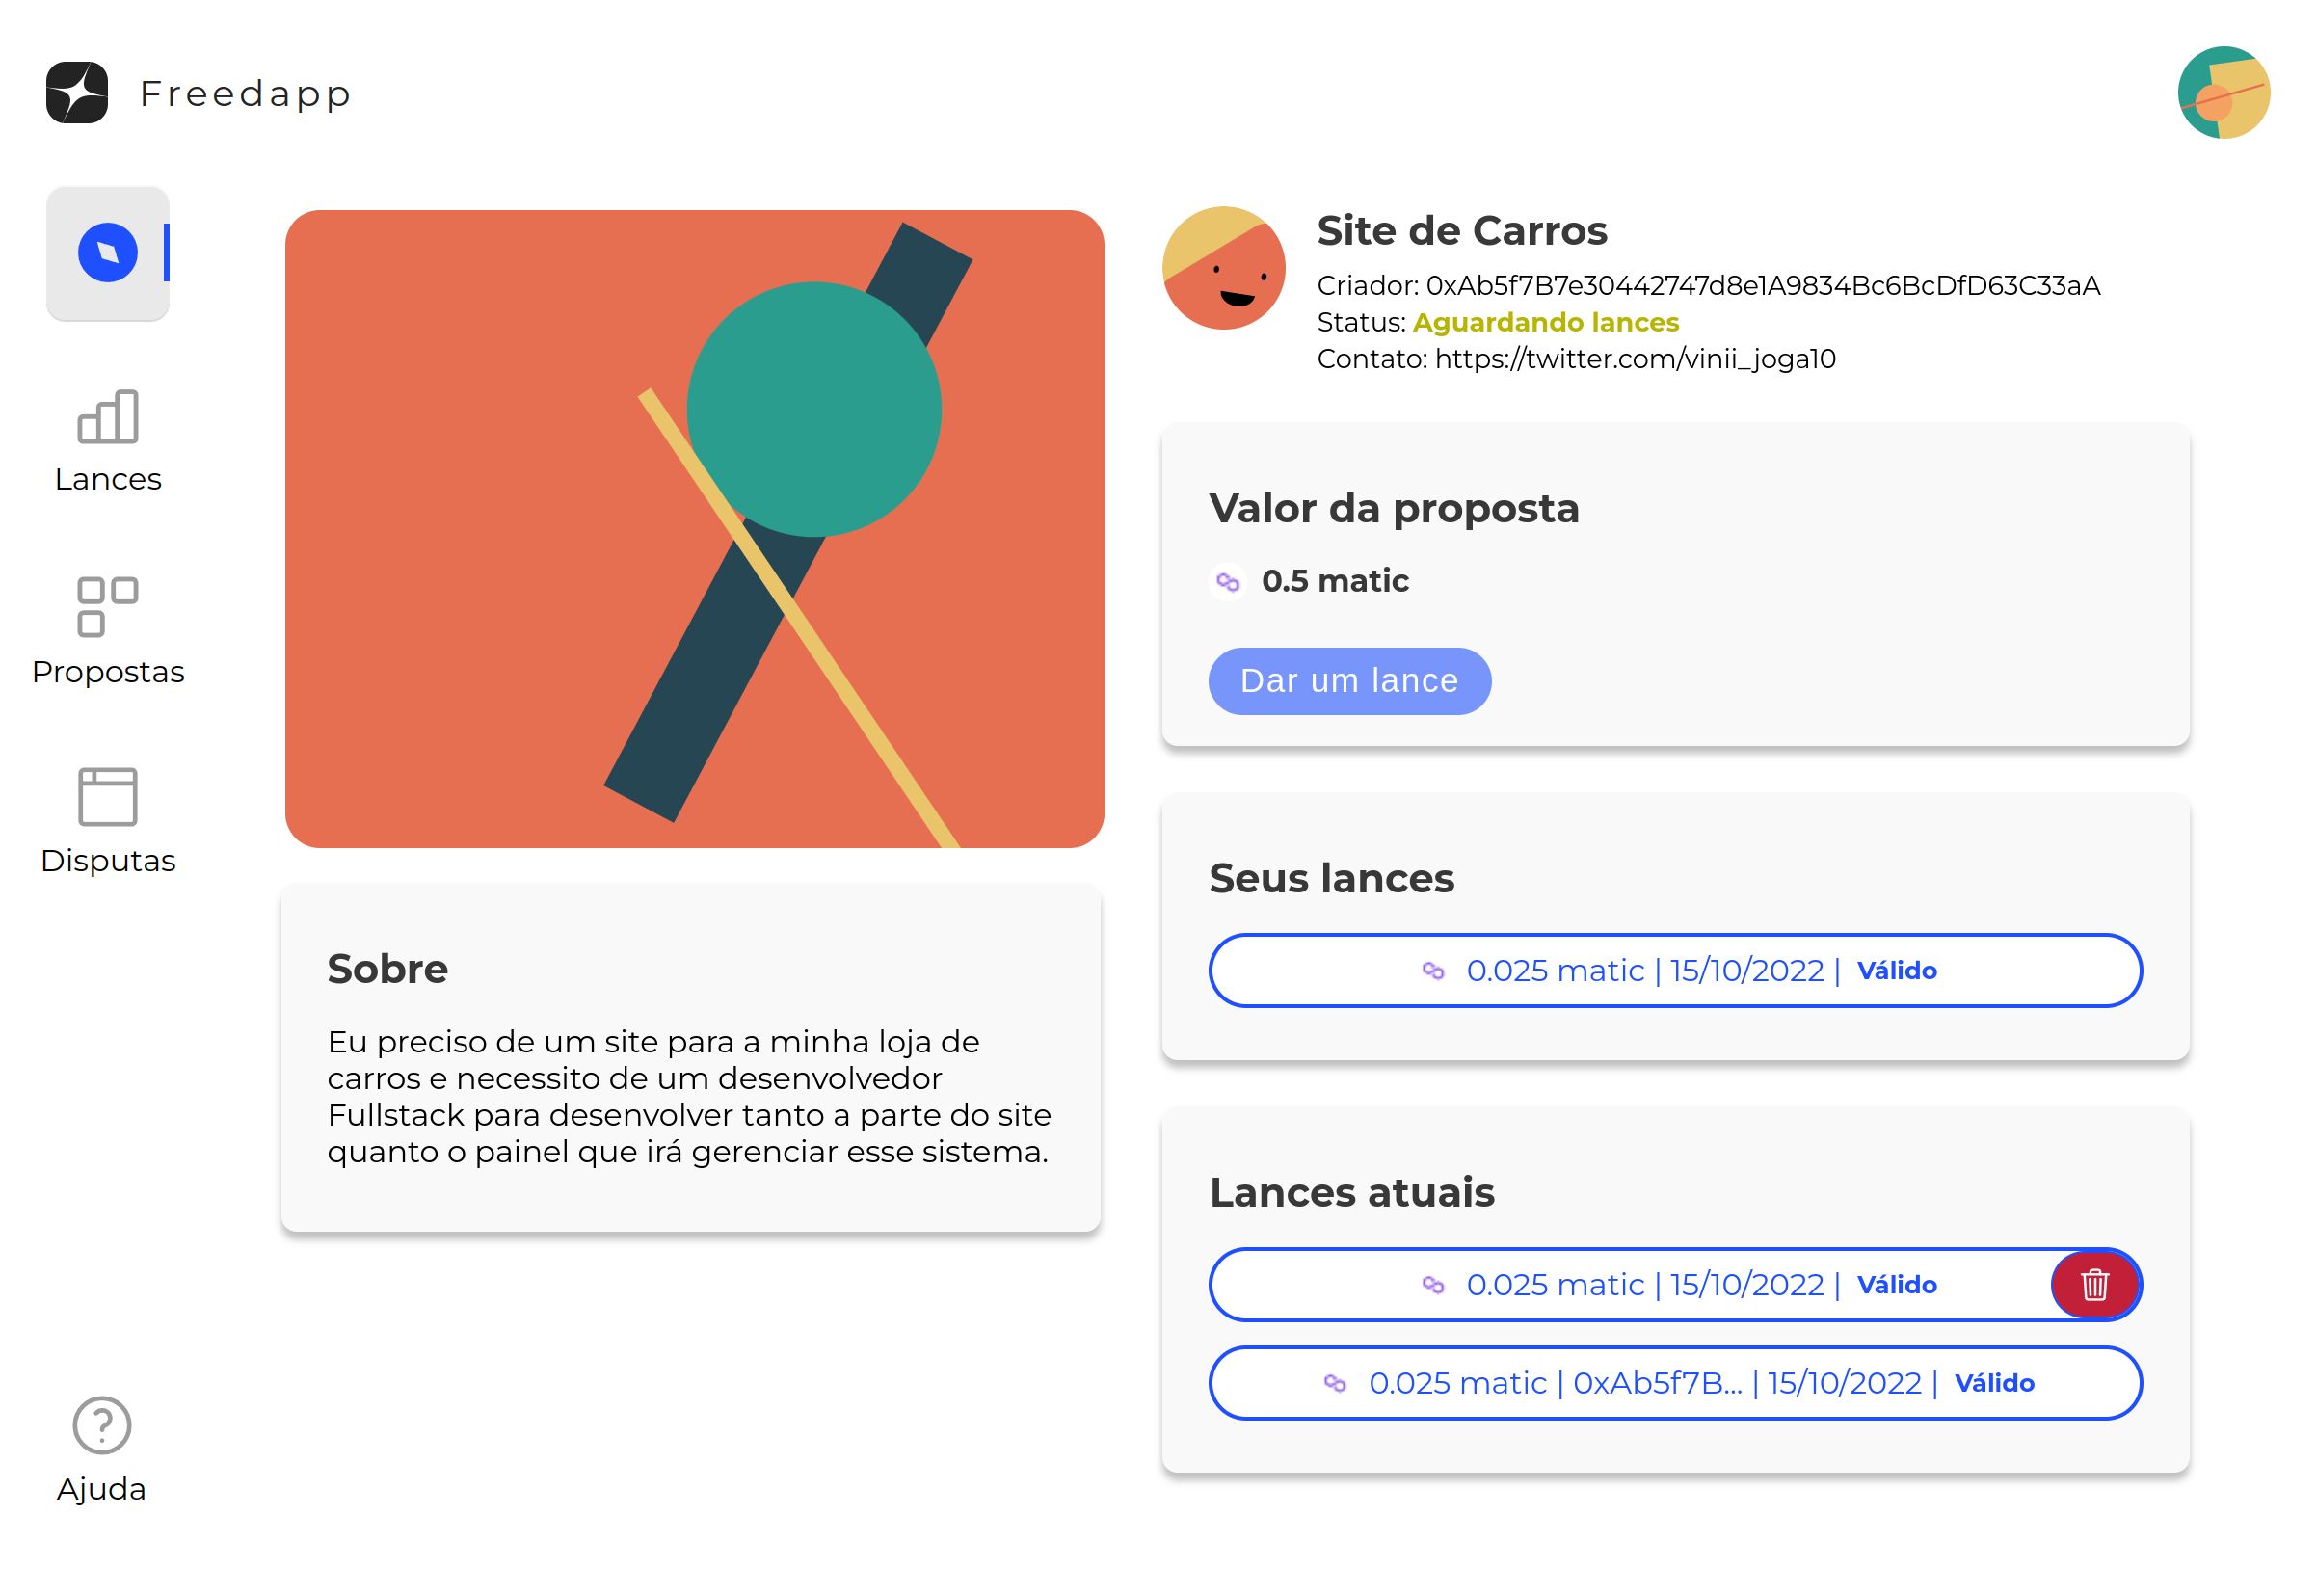
\includegraphics[width=450px]{src/images/app/proposal_detail_see_bid.png}
  \subcaption{Fonte: Autor }
  \label{fig:proposal_detail_see_bid_fig}
\end{figure}

Na página de lances (figura \ref{fig:bid_page_my_bids_fig}), pode-se ver a lista de itens dos lances do usuário logado com informações resumidas igual a tela de início porém com o detalhe do status do lance, caso o lance já tenha sido aceito pelo empregador, aparecerá ''Selecionado'', caso contrário irá continuar aparecendo ''Aguardando lance'' ou ''Rejeitado''. Quando o lance é rejeitado, o freelancer pode ir e recuperar o lance feito, recebendo de volta o valor pago durante a criação do lance.

\begin{figure}[!h]
  \centering
  \caption{Página de listagem de lances}
  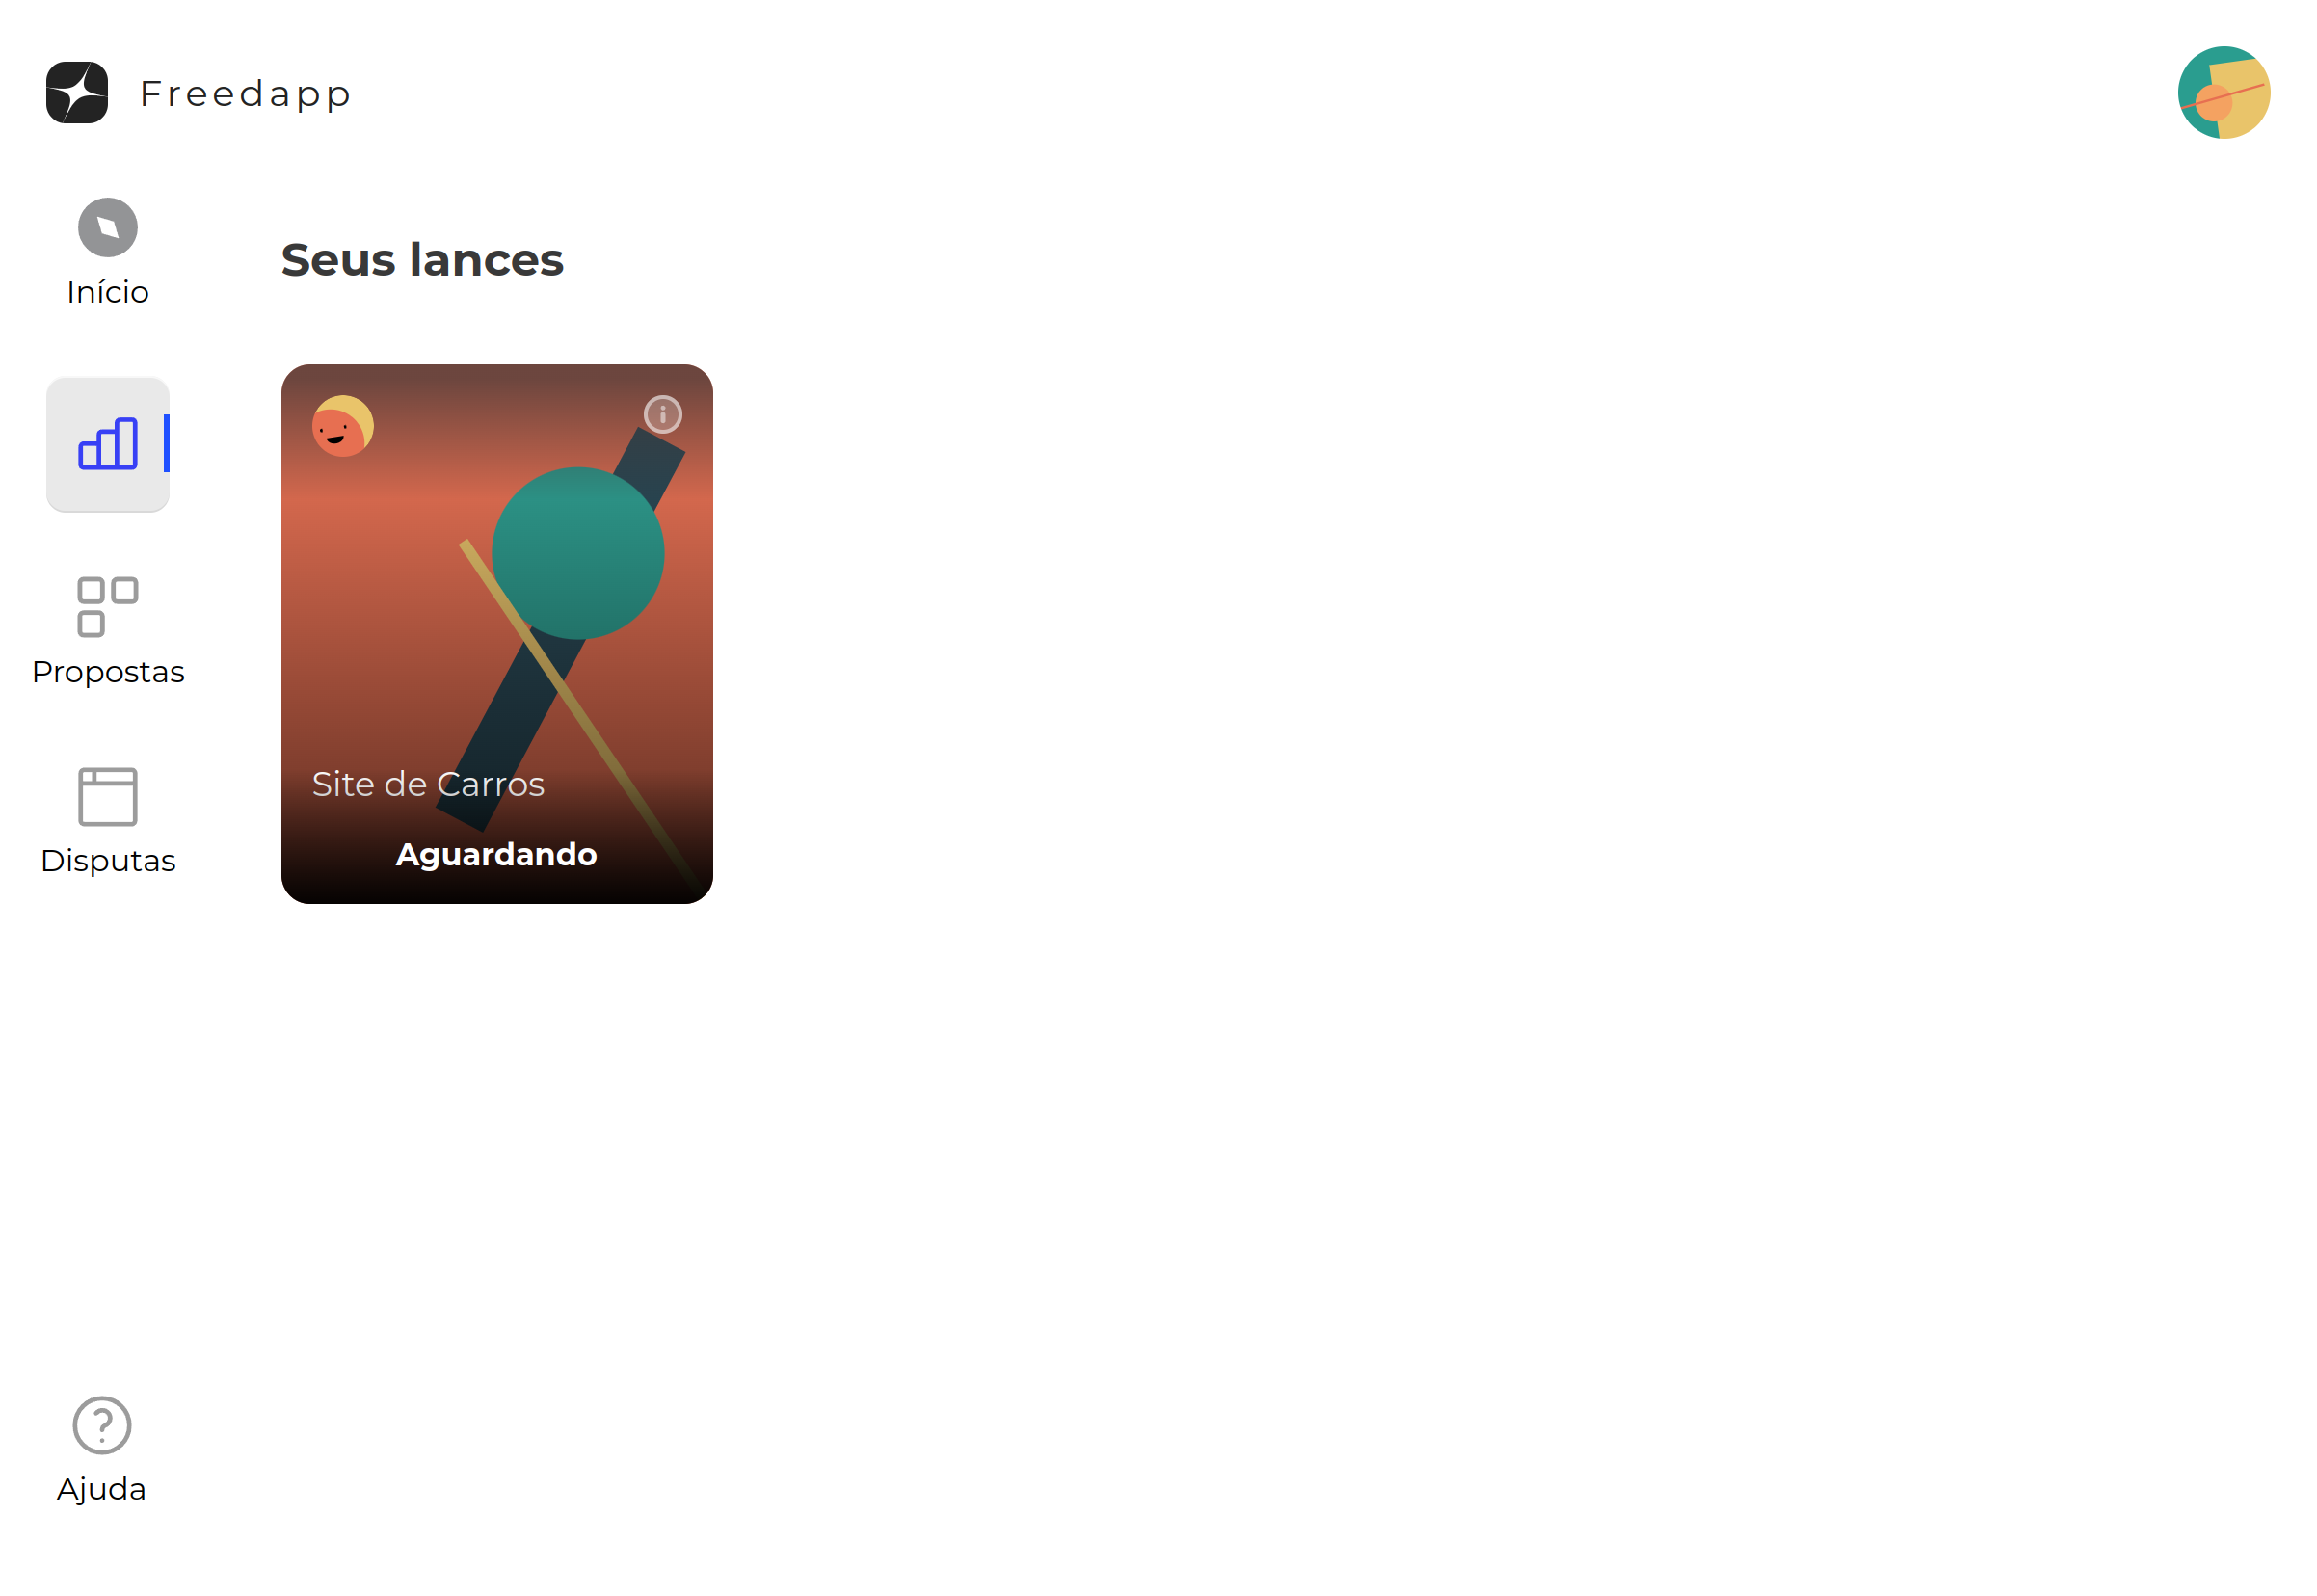
\includegraphics[width=400px]{src/images/app/bid_page_my_bids.png}
  \subcaption{Fonte: Autor }
  \label{fig:bid_page_my_bids_fig}
\end{figure}

Clicando em um lance ainda em progresso, o usuário será redirecionado para a página de detalhes da proposta, com informações da proposta e sua lista de lances e com as informações do seu lance e a possibilidade de remover o lance caso desejado.

Clicando em um lance já aceito, figura \ref{fig:proposal_details_creator_in_development_fig}, além de ver os detalhes da proposta, existe a opção de entrar em disputa com o empregador caso o freelancer achar necessário, ou enviar pagamento caso o freelancer já tenha finalizado o trabalho. Quanto ao botão de entrar em disputa, um novo fluxo é aberto, o qual será comentado mais a frente na parte de disputas.

\begin{figure}[!h]
  \centering
  \caption{Visualizar um lance criado em desenvolvimento}
  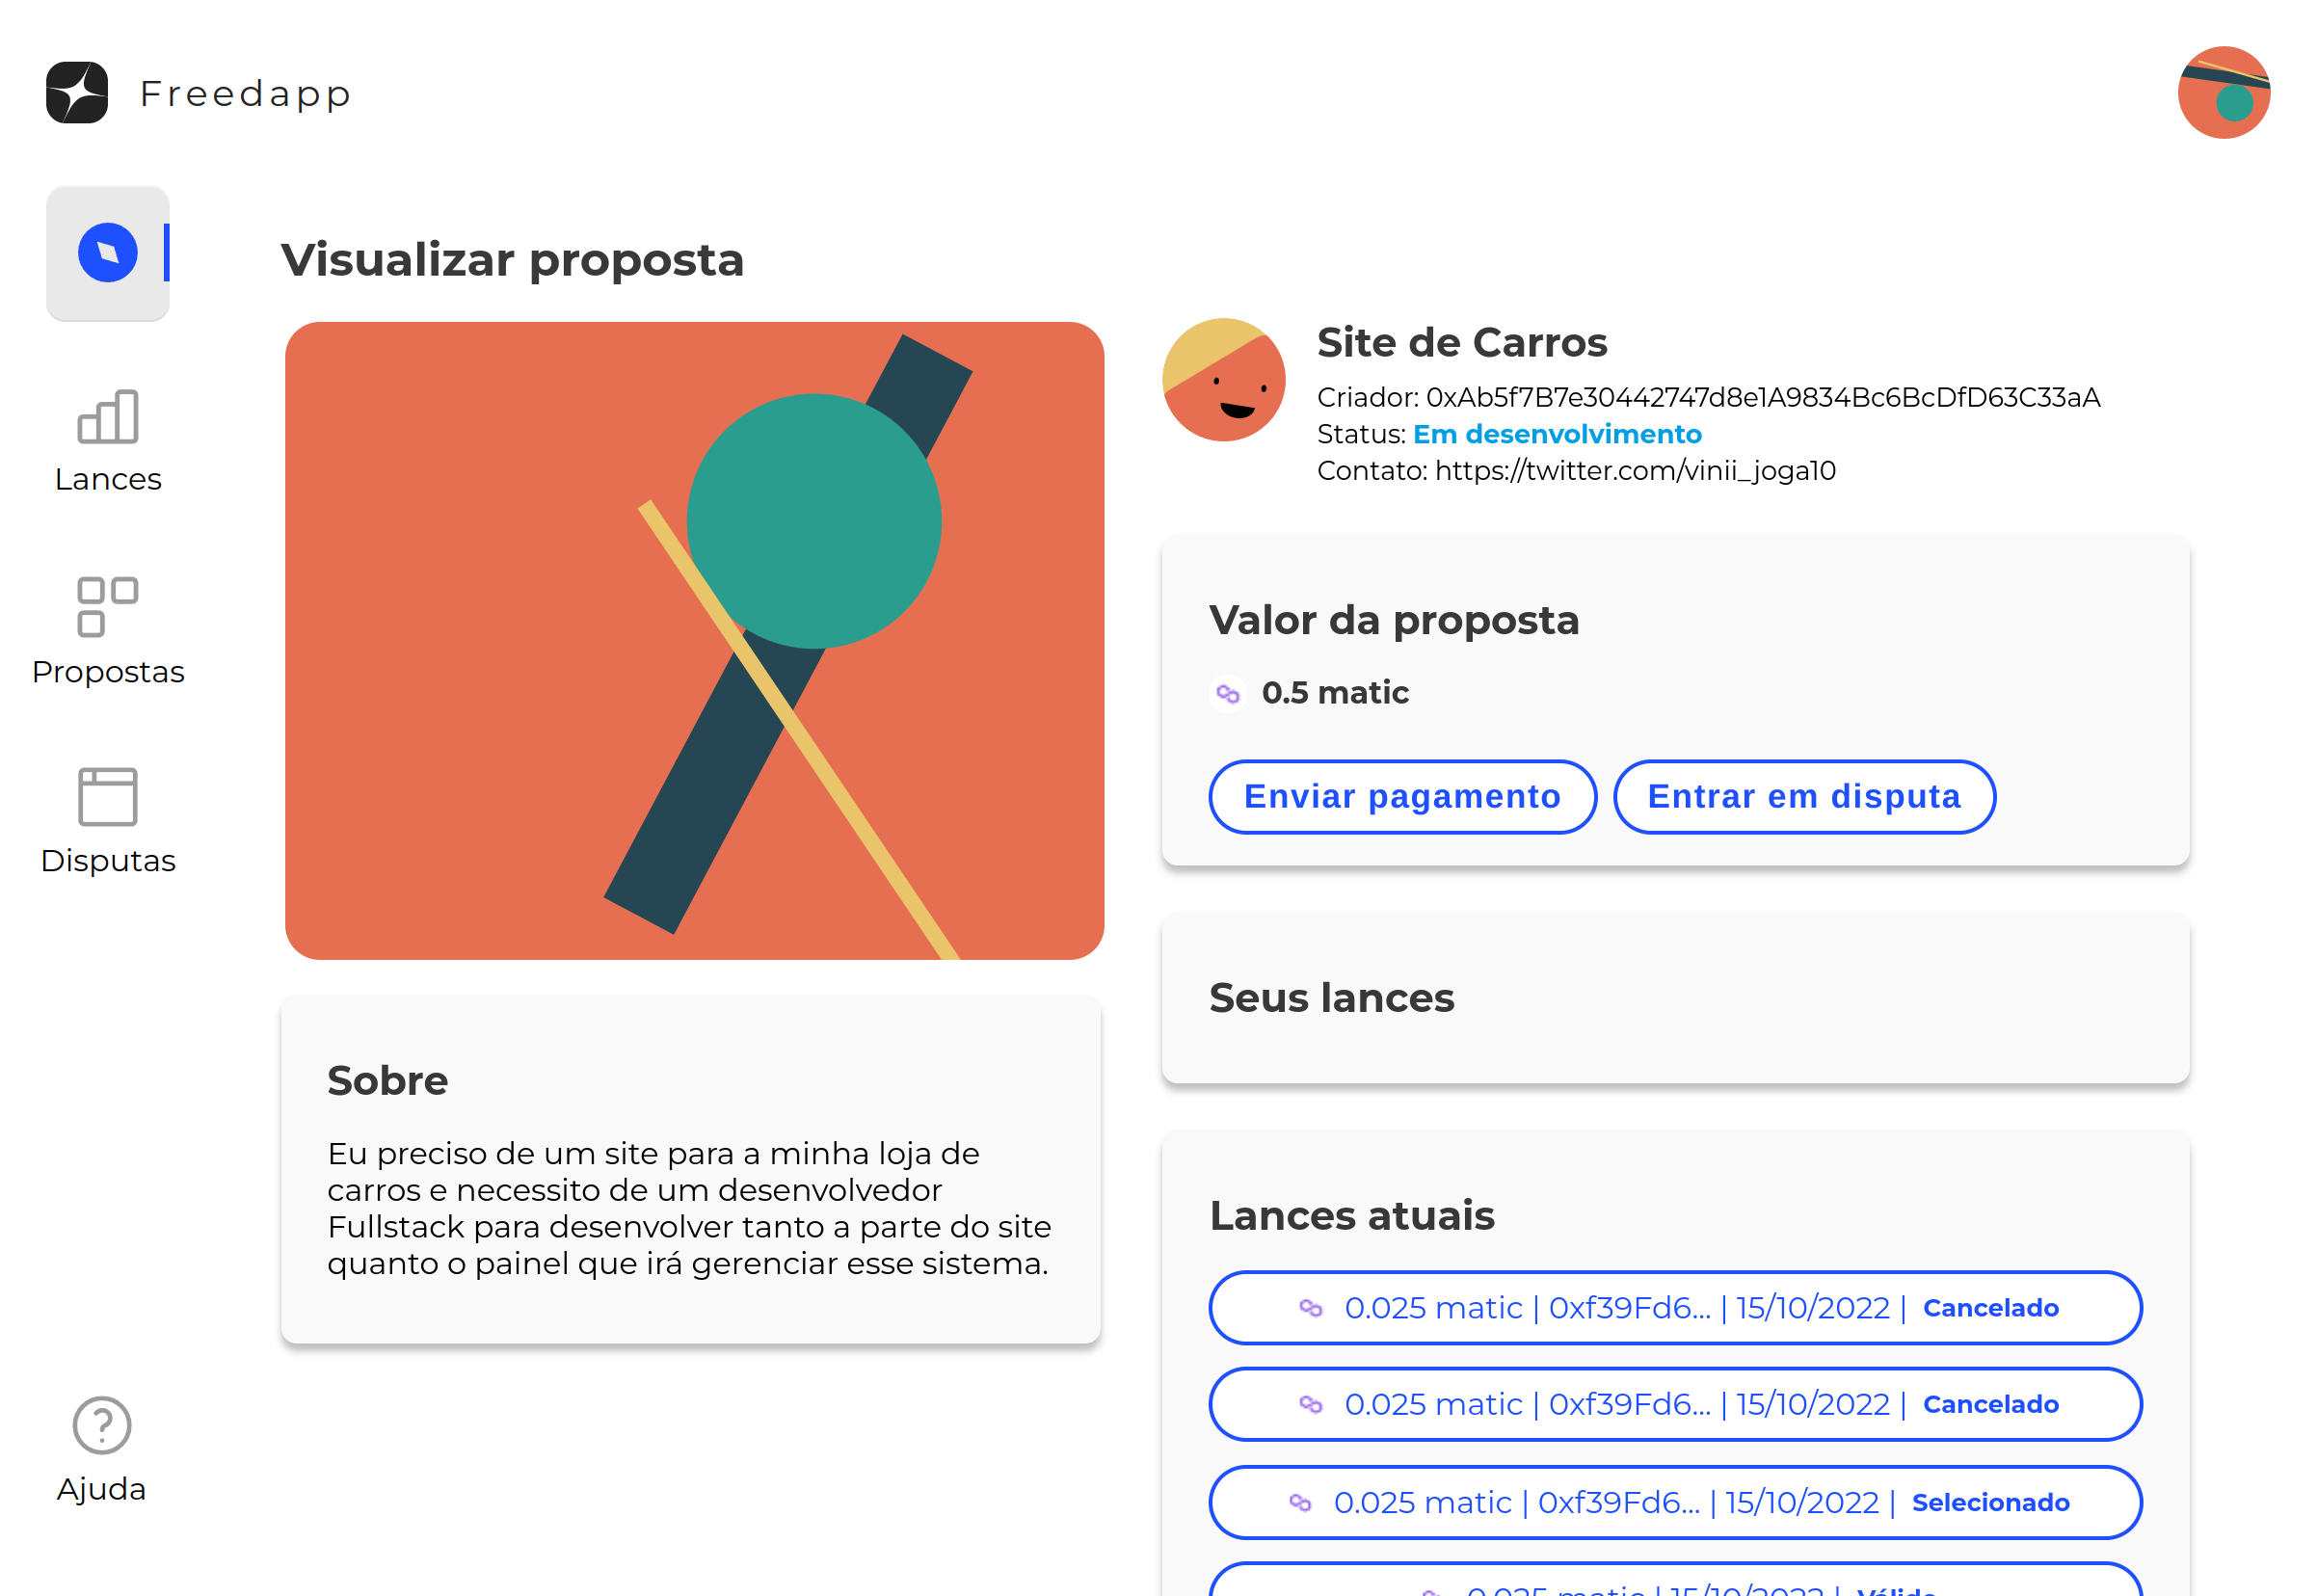
\includegraphics[width=400px]{src/images/app/proposal_details_creator_in_development.png}
  \subcaption{Fonte: Autor }
  \label{fig:proposal_details_creator_in_development_fig}
\end{figure}

Como dito anteriormente, o sistema não cobre a troca de mensagens entre o freelancer e o empregador, deixando opções para aplicativos e sistemas externos, como por exemplo, o e-mail.

Além de toda experiência como usuário freelancer, existe a possibilidade do usuário criar suas próprias propostas, pagando a outros usuário freelancers para executar seus projetos. Na página de proposta, os usuários logados podem ver suas propostas cadastradas com informações resumidas como nome e se a proposta já foi aceita, cancelada ou se continua em progresso, como demonstrado na figura \ref{fig:proposal_list_fig}. Ao clicar em um dos itens da lista de propostas, este é redirecionado para página de detalhes da proposta já descrita anteriormente. 

\begin{figure}[!h]
  \centering
  \caption{Lista da minhas propostas criadas}
  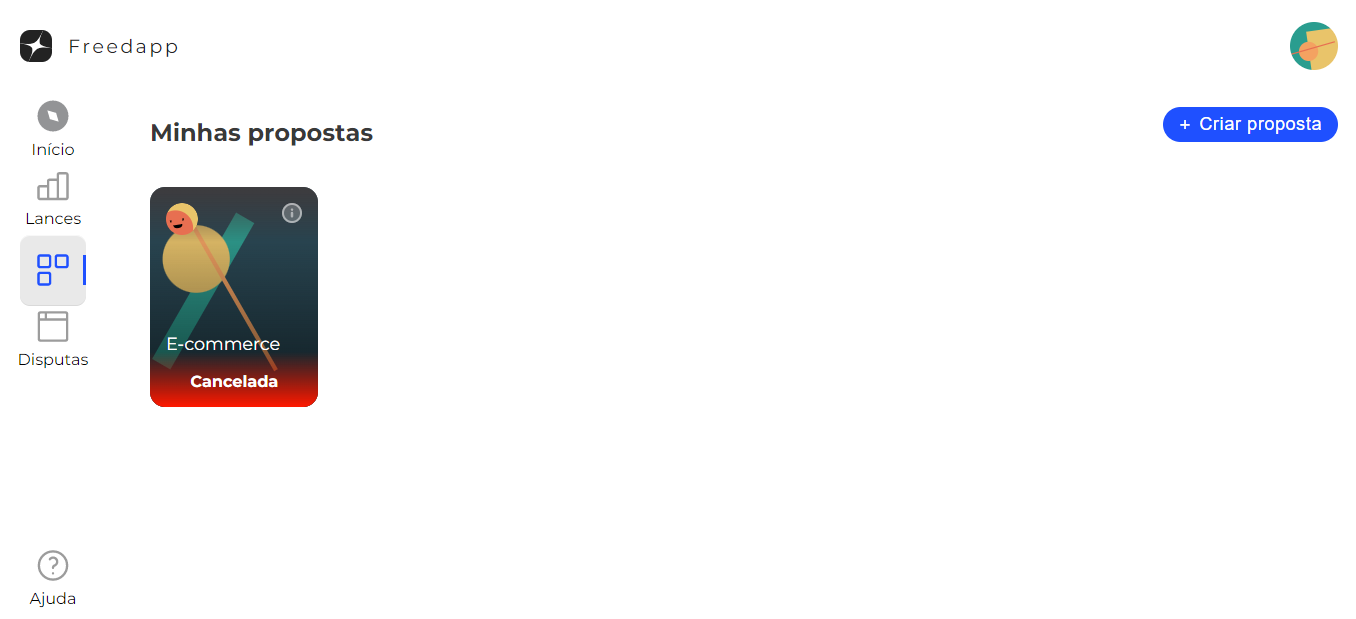
\includegraphics[width=400px]{src/images/app/proposal_list.PNG}
  \subcaption{Fonte: Autor }
  \label{fig:proposal_list_fig}
\end{figure}

Nesta página pode-se criar novas propostas, ao clicar em ''Criar proposta'' no canto superior direito, é aberta uma página de criação, demonstrada na figura \ref{fig:proposal_create_fig}, onde o usuário pode adicionar título/nome, descrição, valor, categoria e as informações de contato do empregador, estas são as informações necessárias para criação de uma proposta.

\begin{figure}[!h]
  \centering
  \caption{Formulário de criação de proposta}
  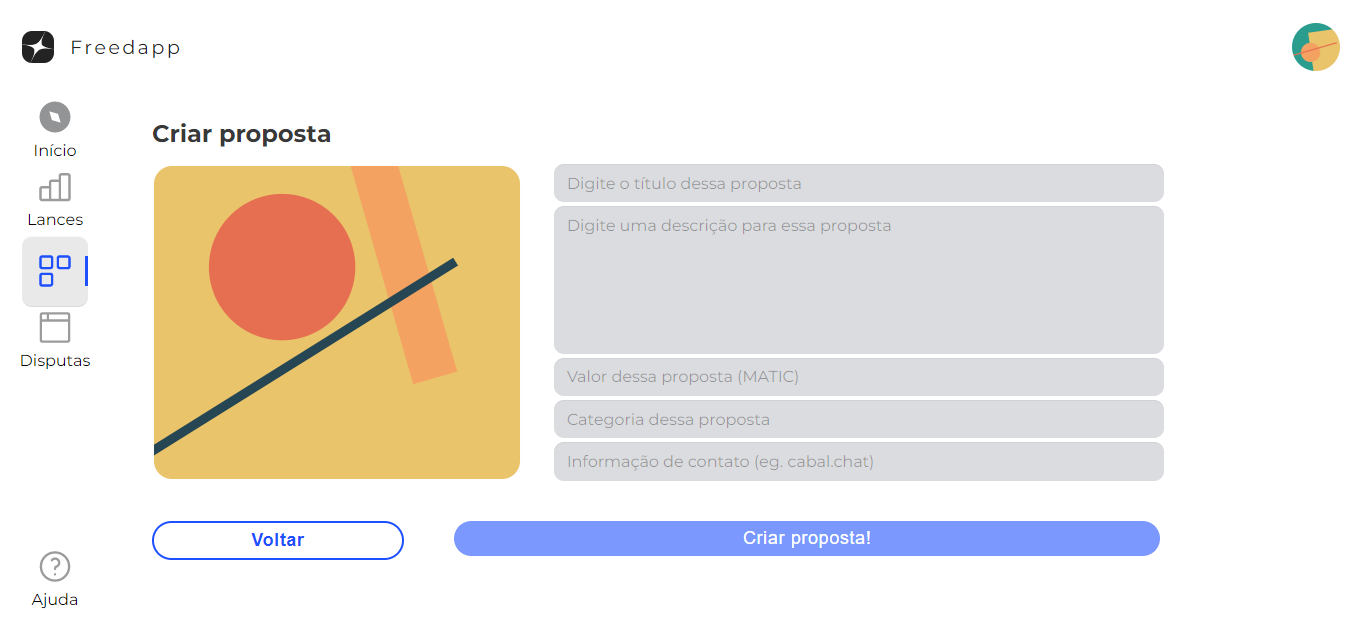
\includegraphics[width=400px]{src/images/app/proposal_create.PNG}
  \subcaption{Fonte: Autor }
  \label{fig:proposal_create_fig}
\end{figure}

A tela de disputas serve para a resolução de conflitos entre os freelancers e os empregados com relação a proposta e os lances. A página lista as disputas que aquele usuário logado participa ou participou, exibindo o nome da proposta e o status da disputa, exemplo na figura \ref{fig:dispute_list_fig}.

\begin{figure}[!h]
  \centering
  \caption{A lista de disputas do usuário}
  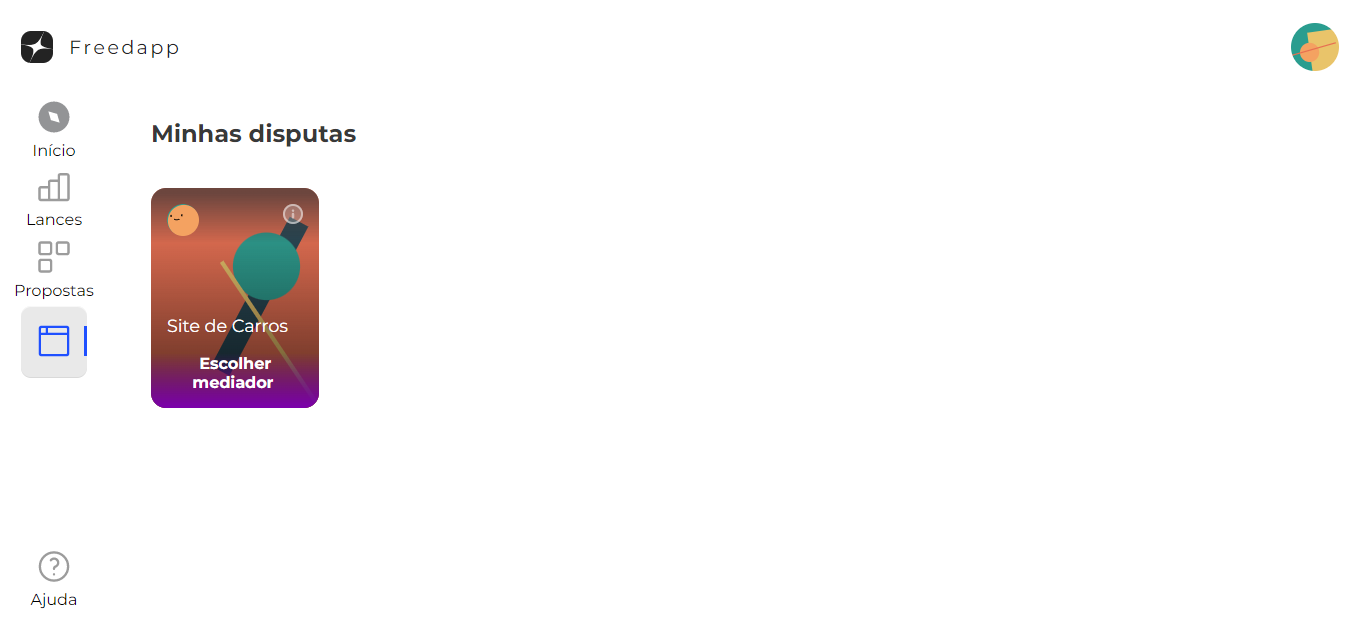
\includegraphics[width=400px]{src/images/app/dispute_list.PNG}
  \subcaption{Fonte: Autor }
  \label{fig:dispute_list_fig}
\end{figure}

Os possíveis status da disputa são:
\begin{itemize}
    \item Escolher mediador
    \item Distribuir valores
    \item Disputa finalizada
\end{itemize}

A disputa inicialmente requer que ambos os lados escolham um mediador, digitando a identificação do mesmo. Para prosseguir para próxima etapa ambos devem escolher o mesmo mediador, portanto, se necessário, há a opção de entrar em contato por meios externos para coordenarem a escolha.

Após o mediador ser escolhido por ambos e acordado, o mediador analisa e pondera os lados, enquanto isso os usuários aguardam a resposta do mediador. Por fim, o mediador diz qual será a porcentagem de saldo distribuído, tanto para o freelancer quanto para o empregador, finalizando a disputa. O mediador ganha uma taxa de 5\% do valor total transacionado como incentivo para realizar seu trabalho de mediador. As figuras \ref{fig:dispute_mediator_list_fig} e \ref{fig:dispute_mediator_values_fig} mostram a visão do mediador.

\begin{figure}[!h]
  \centering
  \caption{As disputas na visão do mediador}
  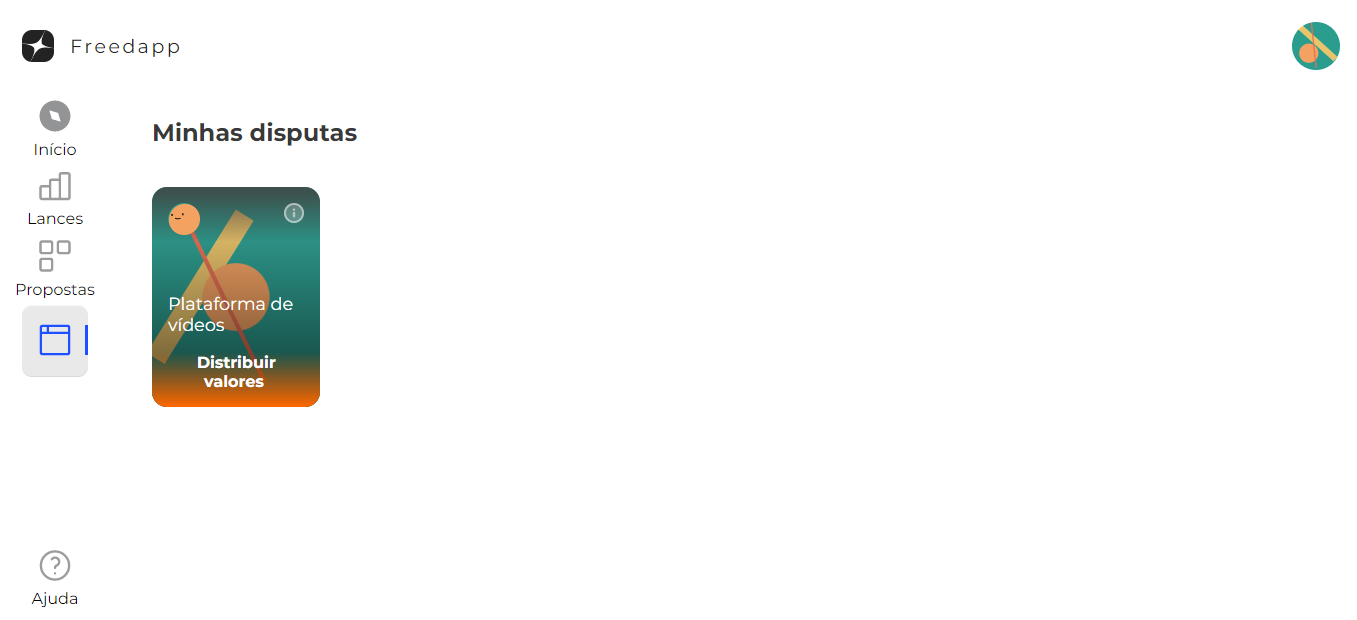
\includegraphics[width=400px]{src/images/app/dispute_mediator_list.PNG}
  \subcaption{Fonte: Autor }
  \label{fig:dispute_mediator_list_fig}
\end{figure}

\begin{figure}[!h]
  \centering
  \caption{O mediador distribuindo valores}
  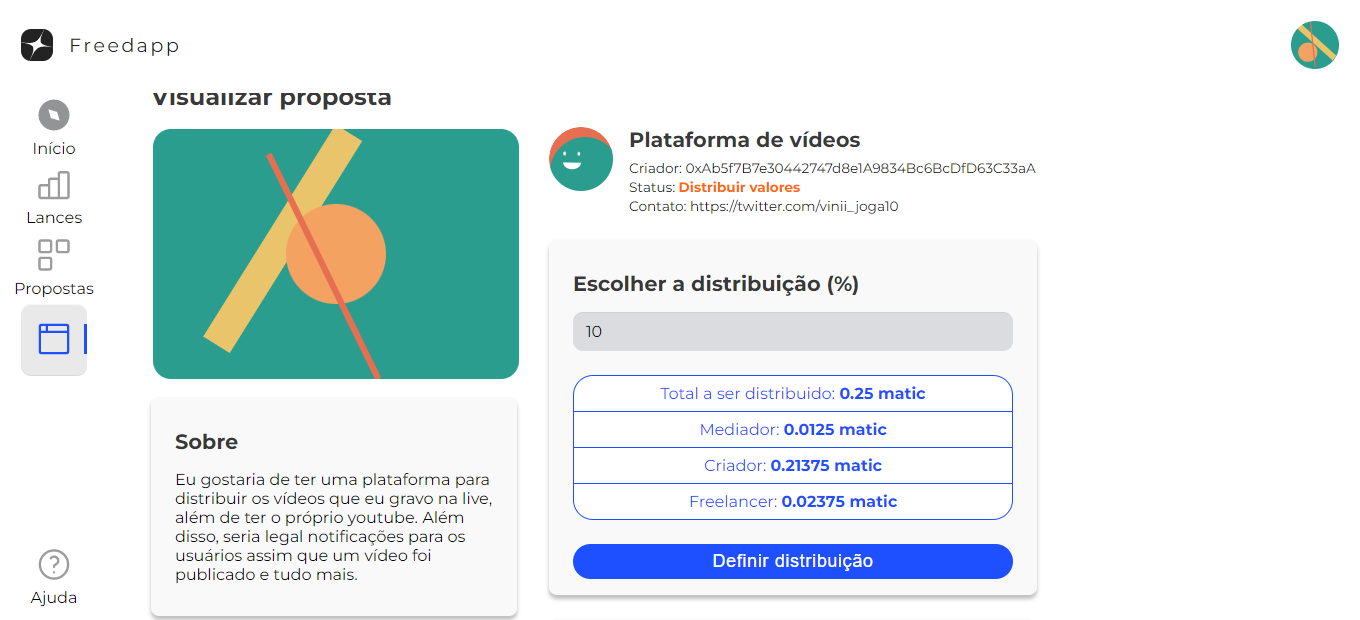
\includegraphics[width=400px]{src/images/app/dispute_mediator_values.PNG}
  \subcaption{Fonte: Autor }
  \label{fig:dispute_mediator_values_fig}
\end{figure}

Após concluída a distribuição de valores pelo mediator a disputa é finalizada e os valores do freelancer e o do empregador são automaticamente transferidos. Agora, após o processo de disputa, na lista de disputas do usuário, a proposta consta como ''Finalizada'' como mostrado na figura \ref{fig:dispute_finish_fig}.

\begin{figure}[!h]
  \centering
  \caption{Lista de disputas do usuário}
  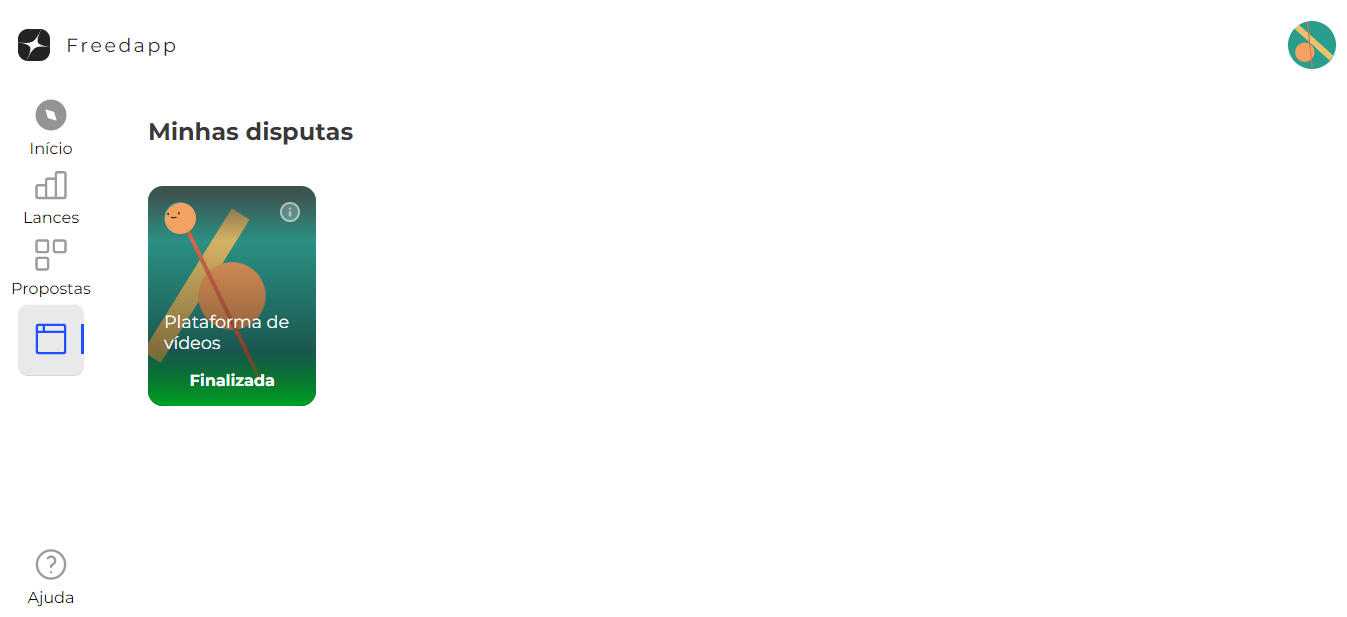
\includegraphics[width=400px]{src/images/app/dispute_finish.PNG}
  \subcaption{Fonte: Autor }
  \label{fig:dispute_finish_fig}
\end{figure}

Por fim, temos a tela de ajuda, que tem por objeto sanar as dúvidas dos usuários e mostrar como funciona o FreedApp, além de possuir tutoriais, como por exemplo ''Como instalar o MetaMask''.

\section{Smart Contracts}

Assim como no caso do site, os \textit{Smart Contracts} foram hospedados na rede de teste da \textit{Polygon} chamada \textit{Mumbai}, e assim como planejado no desenvolvimento, foi hospedado três contratos com os seguintes endereços:

\begin{itemize}
    \item Proposta: \textit{0x0672C724765Ca66BB9325881A7ACA1dfB3854137}
    \item Lances: \textit{0xEEa3e8974C2f631D4E0351F5f30997fD311633C0}
    \item Disputas: \textit{0x84262946Bc86229D12D0F17C5F60726E760Ef3Ff}
\end{itemize}

Os contratos não possuem uma representação visual assim como um site mas a seguir será mostrado um pouco do código usado, assim como, as técnicas que foi utilizado para evitar o problema de \textit{Reentrancy}.

\subsection{Propostas}

O contrato de propostas interliga outros contratos além de realizar as operações básicas de propostas, sendo assim, o principal da aplicação desenvolvida. O contrato de proposta foi dividido em três sub-contratos definidos pelas interfaces de \textit{IProposalBase}, \textit{IProposalPermission} e \textit{IProposalCore}, responsáveis por operações básicas, validação de permissão e as operações principais, respectivamente.

A seguir, na figura \ref{fig:proposal_core_contract_fig}, alguns dos métodos disponíveis na interface do \textit{IProposalCore}. Pode-se observar diversos métodos com o prefixo ''\textit{on}'' como \textit{onBidderSelected} e \textit{onCreateDispute}. Esses métodos são usados para a comunicação entre outros contratos, sendo mais específico, para a comunicação do contrato de Lances e Disputas, para que o contrato de proposta seja atualizado quando, por exemplo, um lance for selecionado ou uma disputa for criada.

\begin{figure}[!h]
  \centering
  \caption{Interface do Contrato Core de Proposta}
  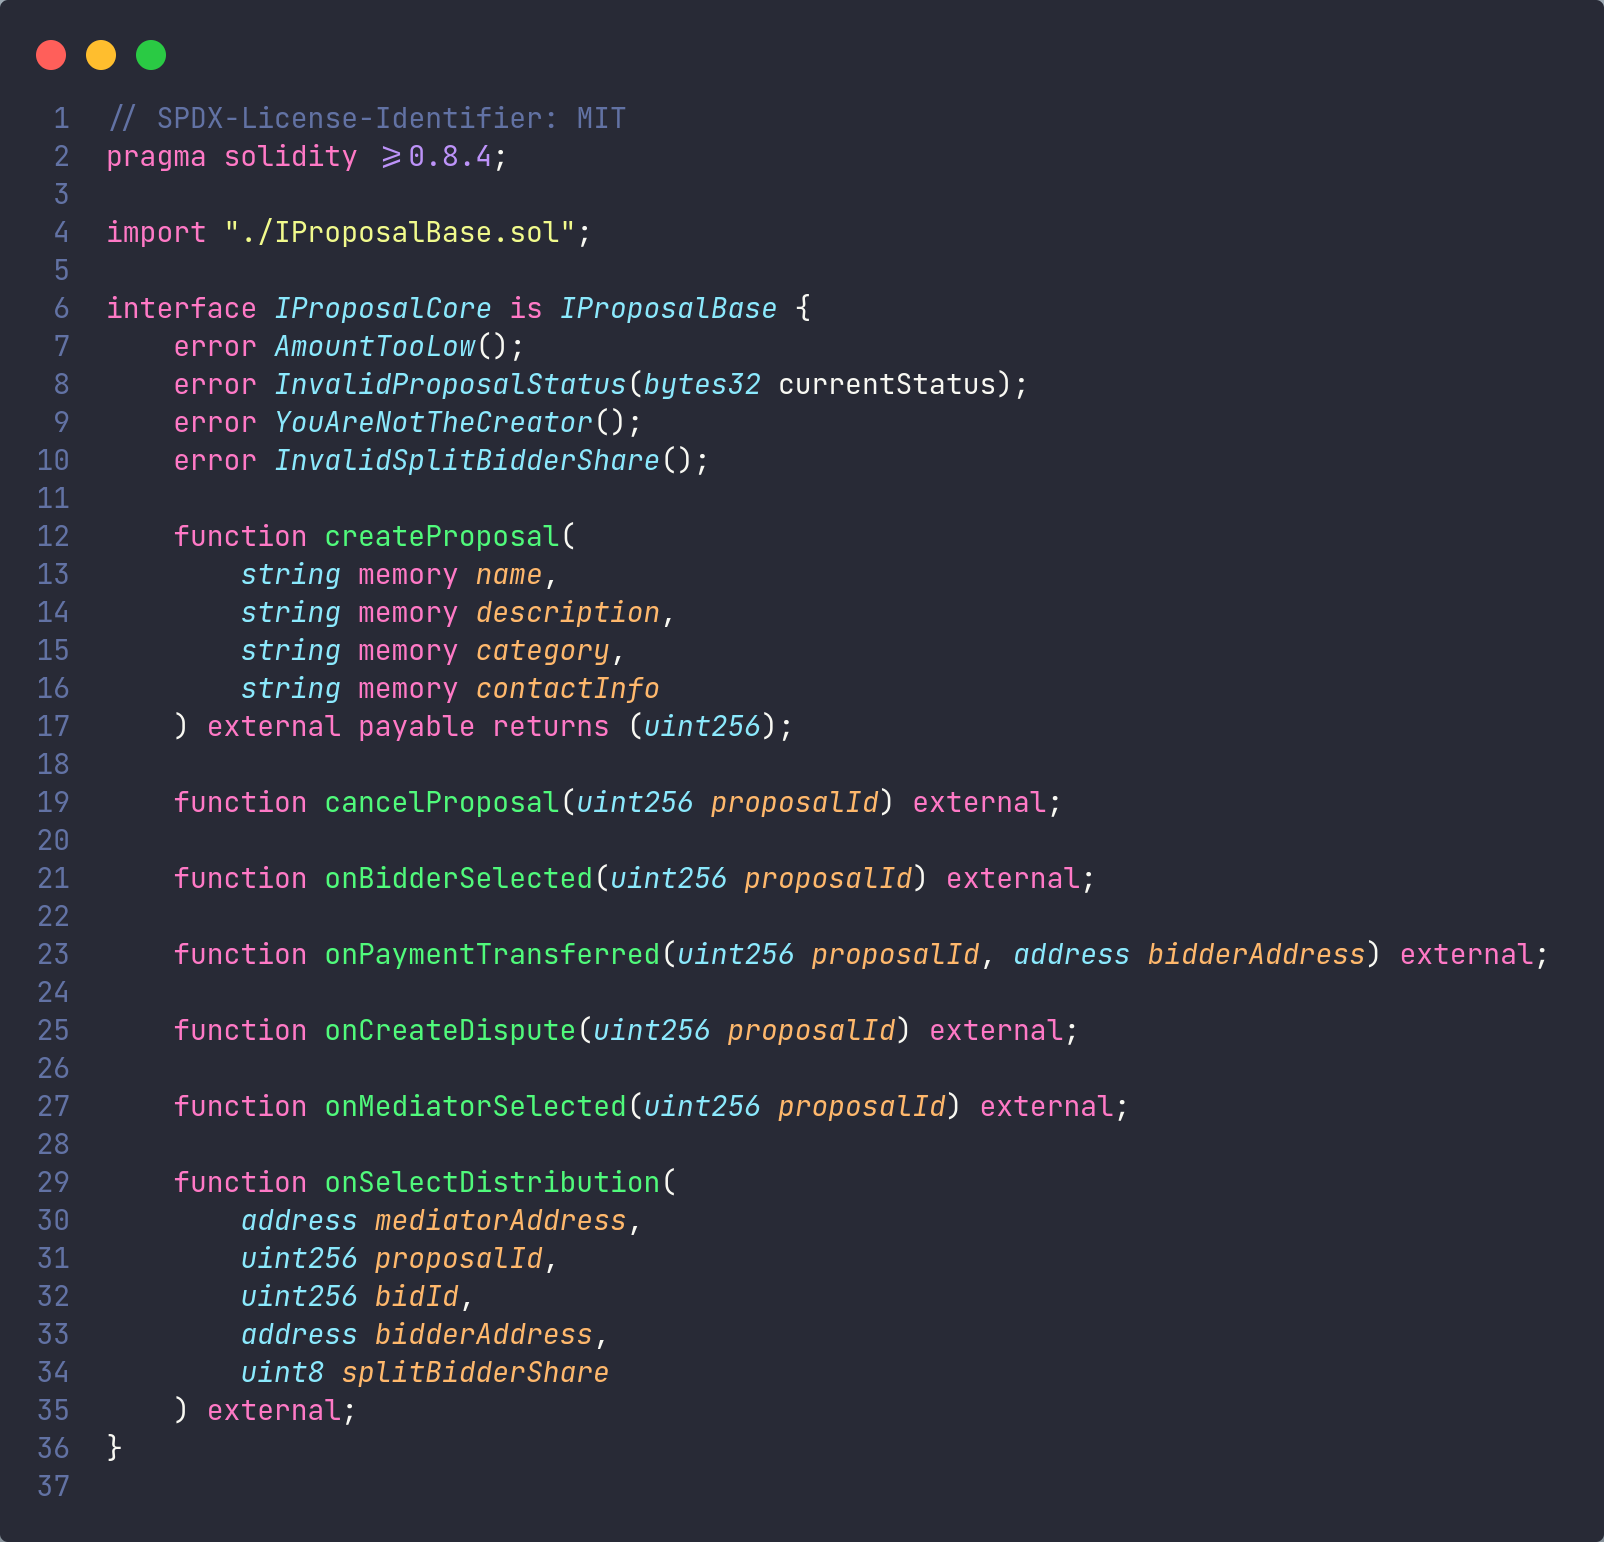
\includegraphics[width=320px]{src/images/contracts/proposal_core_contract.png}
  \subcaption{Fonte: Autor }
  \label{fig:proposal_core_contract_fig}
\end{figure}

Além dessa interface, há mais uma para representar as operações mais básicas de uma proposta, conforme mostrado na figura \ref{fig:proposal_base_contract_fig}. É interessante notar nos métodos como não há uma forma de retornar uma lista de propostas. Isso é pensado de forma proposital, e como descrito no desenvolvimento, é uma estratégia para economizar \textit{Gas} e reduzir custos da rede.

\begin{figure}[!h]
  \centering
  \caption{Interface do Contrato Base de Proposta}
  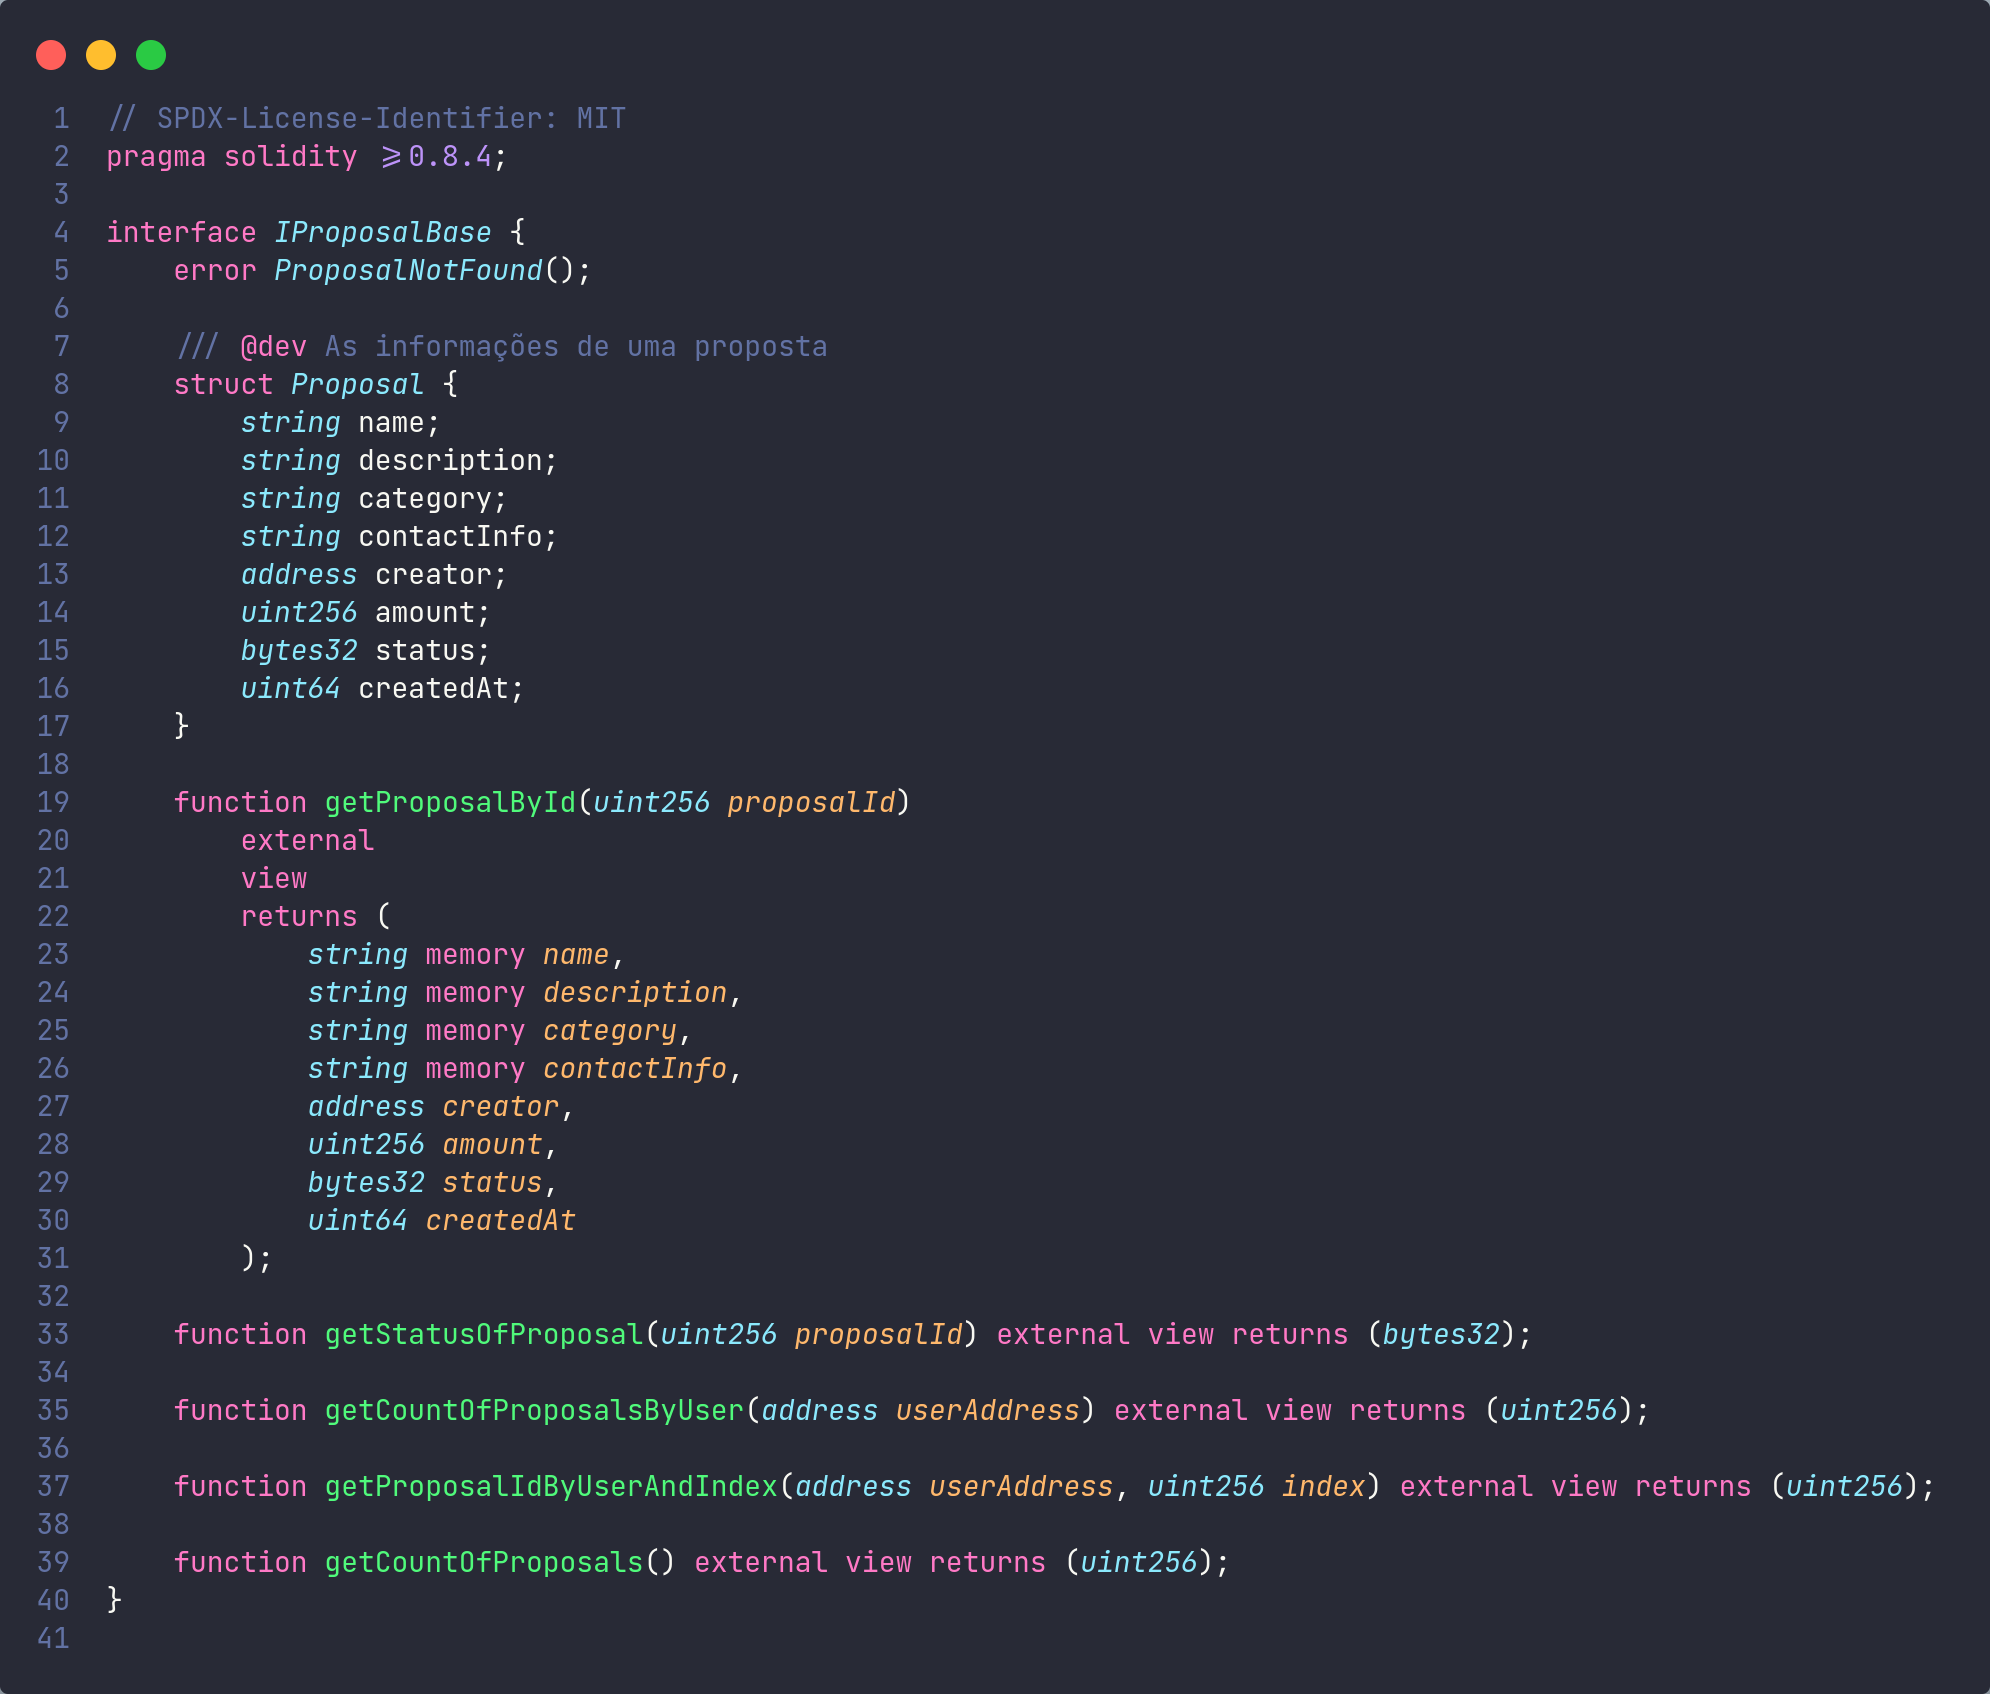
\includegraphics[width=320px]{src/images/contracts/proposal_base_contract.png}
  \subcaption{Fonte: Autor }
  \label{fig:proposal_base_contract_fig}
\end{figure}

Para que o usuário possa listar as propostas criadas no contrato, é necessário realizar duas operações básicas: \textit{getCountOfProposals} para saber quantas propostas existem e depois chamar o método \textit{getProposalById} para obter as informações da proposta. 

A identificação da proposta é incremental e começa em 1, dessa forma, se a contagem retornar 10, pode-se presumir com segurança que poderá obter as propostas com os \textit{IDs} de 1 a 10. Caso o usuário passe a identificação de uma proposta que não exista, é lançado um erro para alertar que não foi encontrado.

E por fim, para que o contrato de proposta saiba se deve ou não aceitar executar um método que é protegido para ser executado apenas pelo contrato de Lances ou Disputas, é usado a interface mostrado na figura \ref{fig:proposal_permission_contract_fig}.

\begin{figure}[!h]
  \centering
  \caption{Interface do Contrato Permission de Proposta}
  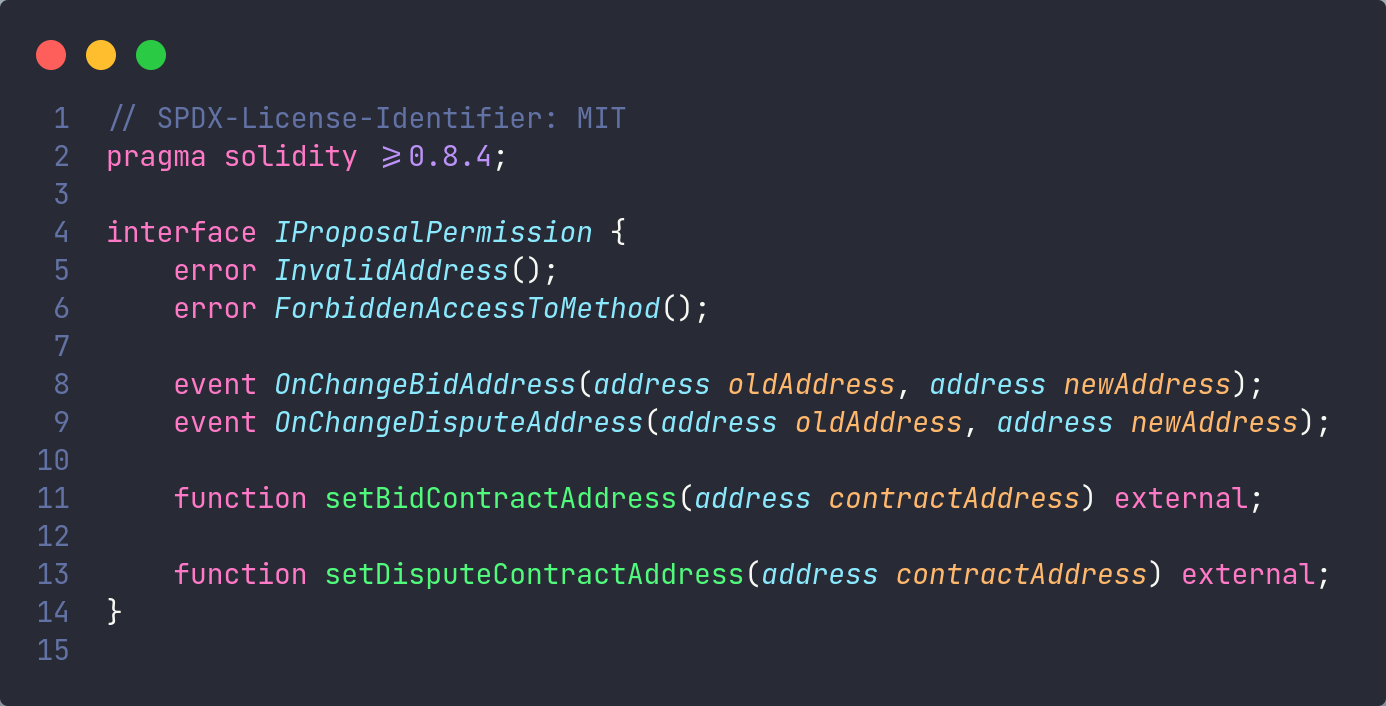
\includegraphics[width=320px]{src/images/contracts/proposal_permission_contract.png}
  \subcaption{Fonte: Autor }
  \label{fig:proposal_permission_contract_fig}
\end{figure}

Na figura \ref{fig:proposal_permission_contract_fig}, pode-se notar dois métodos no qual podem ser usados para especificar o endereço dos contratos de Lance e Disputa, dessa forma, quando o método for executado, bastaria checar se quem está executando bate com o endereço salvo no contrato de proposta.

Até esse ponto, o que foi mostrado é apenas o que foi exposto para o site consumir, quanto a sua implementação interna, será mostrado alguns trechos principais. Para começar, para solucionar o problema de \textit{Reentrancy}, o método de pagamento foi escrito como mostra a figura \ref{fig:proposal_core_on_payment_transferred_fig}.

\begin{figure}[!h]
  \centering
  \caption{Trecho de código do método onPaymentTransferred}
  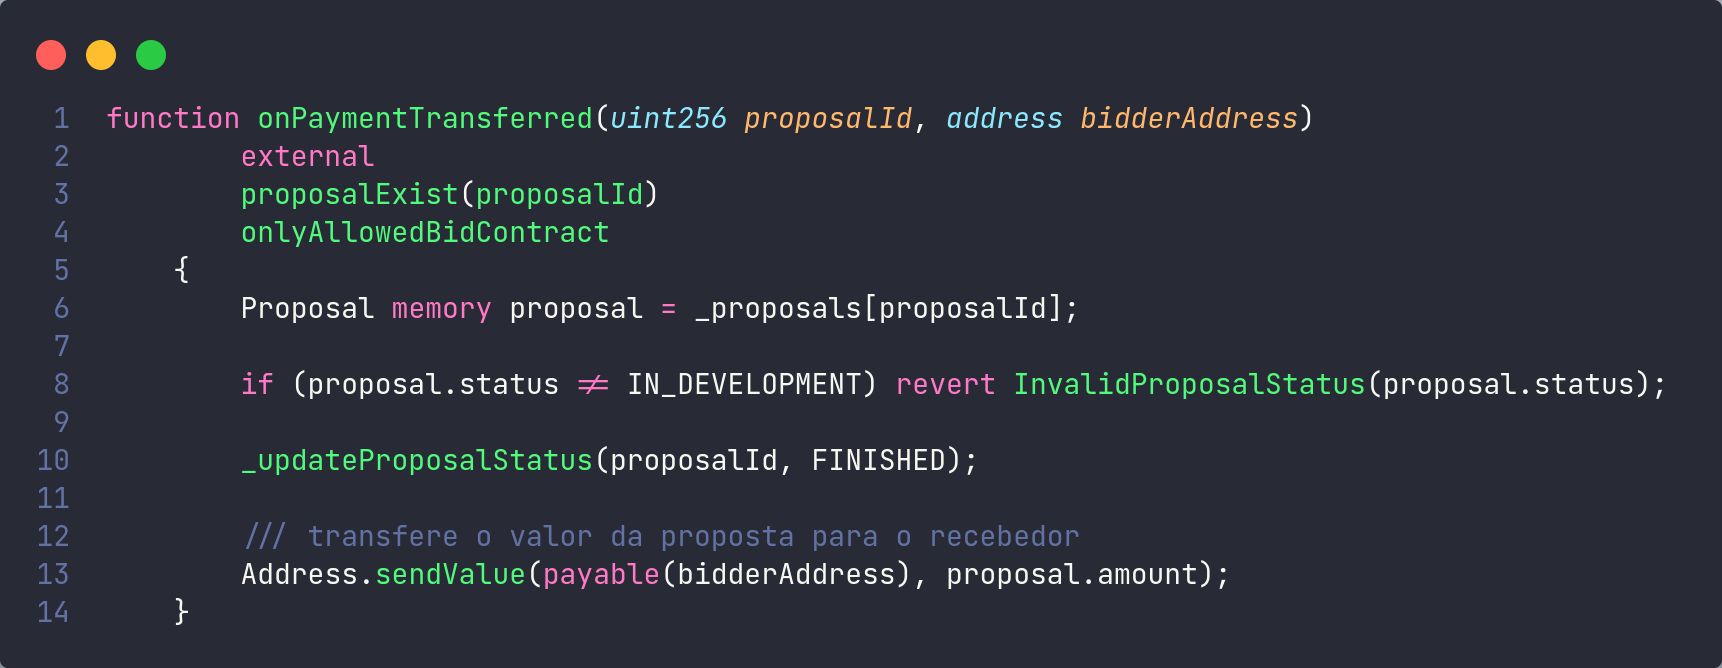
\includegraphics[width=350px]{src/images/contracts/proposal_core_on_payment_transferred.png}
  \subcaption{Fonte: Autor }
  \label{fig:proposal_core_on_payment_transferred_fig}
\end{figure}

Pode-se observar na linha 8 da figura \ref{fig:proposal_core_on_payment_transferred_fig}, a verificação do \textit{status} da proposta, só passará daquela verificação se o \textit{status} for igual \textit{IN\_DEVELOPMENT}, que significa que está em desenvolvimento. Após passar na verificação, imediatamente é chamado a função \textit{\_updateProposalStatus} que irá atualizar o \textit{status} da proposta para \textit{FINISHED}.

Dessa forma, esse método não poderá ser chamado novamente sem lançar o erro de \textit{InvalidProposalStatus}. Assim, o contrato é protegido de pessoas má intencionadas que buscam falhas para roubar todo o dinheiro do contrato.

Por fim, como medidas de segurança adicionais, o \textit{Solidity} possui a funcionalidade chamada \textit{Modifiers}, onde é criado uma função para validar se deve ou não executar o método em questão. Na função de \textit{onPaymentTransferred}, há dois \textit{Modifiers}: \textit{proposalExist} para checar se a proposta existe e \textit{onlyAllowedBidContract} que assegura que esse método só execute caso quem esteja chamando ele seja o contrato de Lances.

\subsection{Lances}

Após o contrato de propostas, o contrato de lances será um dos mais usados e ele foi dividido, assim como o contrato de propostas, em três sub-contratos chamados de \textit{IBidCore}, \textit{IBidBase} e o contrato \textit{BidProposal}, responsáveis por operações básicas, interação entre lance-proposta e ações principais, respectivamente.

A seguir, na figura \ref{fig:bid_core_contract_fig} pode-se observar alguns dos métodos disponíveis na interface de \textit{IBidCore}.

\begin{figure}[!h]
  \centering
  \caption{Interface do contrato IBidCore de Lances}
  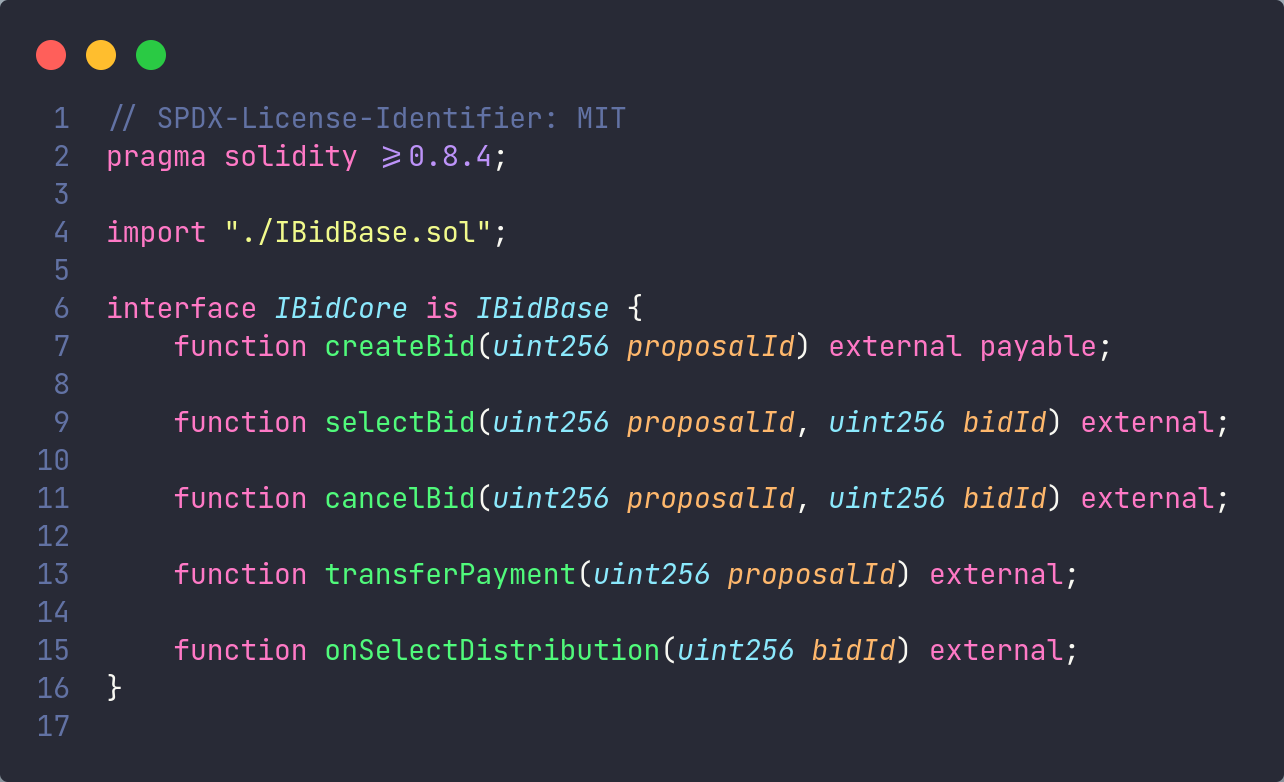
\includegraphics[width=320px]{src/images/contracts/bid_core.png}
  \subcaption{Fonte: Autor }
  \label{fig:bid_core_contract_fig}
\end{figure}

Assim como em propostas, o contrato de \textit{IBidCore} possui alguns métodos com a intenção de ser usado por outros contratos, no caso, o \textit{onSelectDistribution} tem a intenção de ser usado pelo contrato de disputas.

Após isso, como é ilustrado na figura \ref{fig:bid_base_contract_fig}, a interface \textit{IBidBase} do contrato base de lances.

\begin{figure}[!h]
  \centering
  \caption{Interface do contrato Base de Lances}
  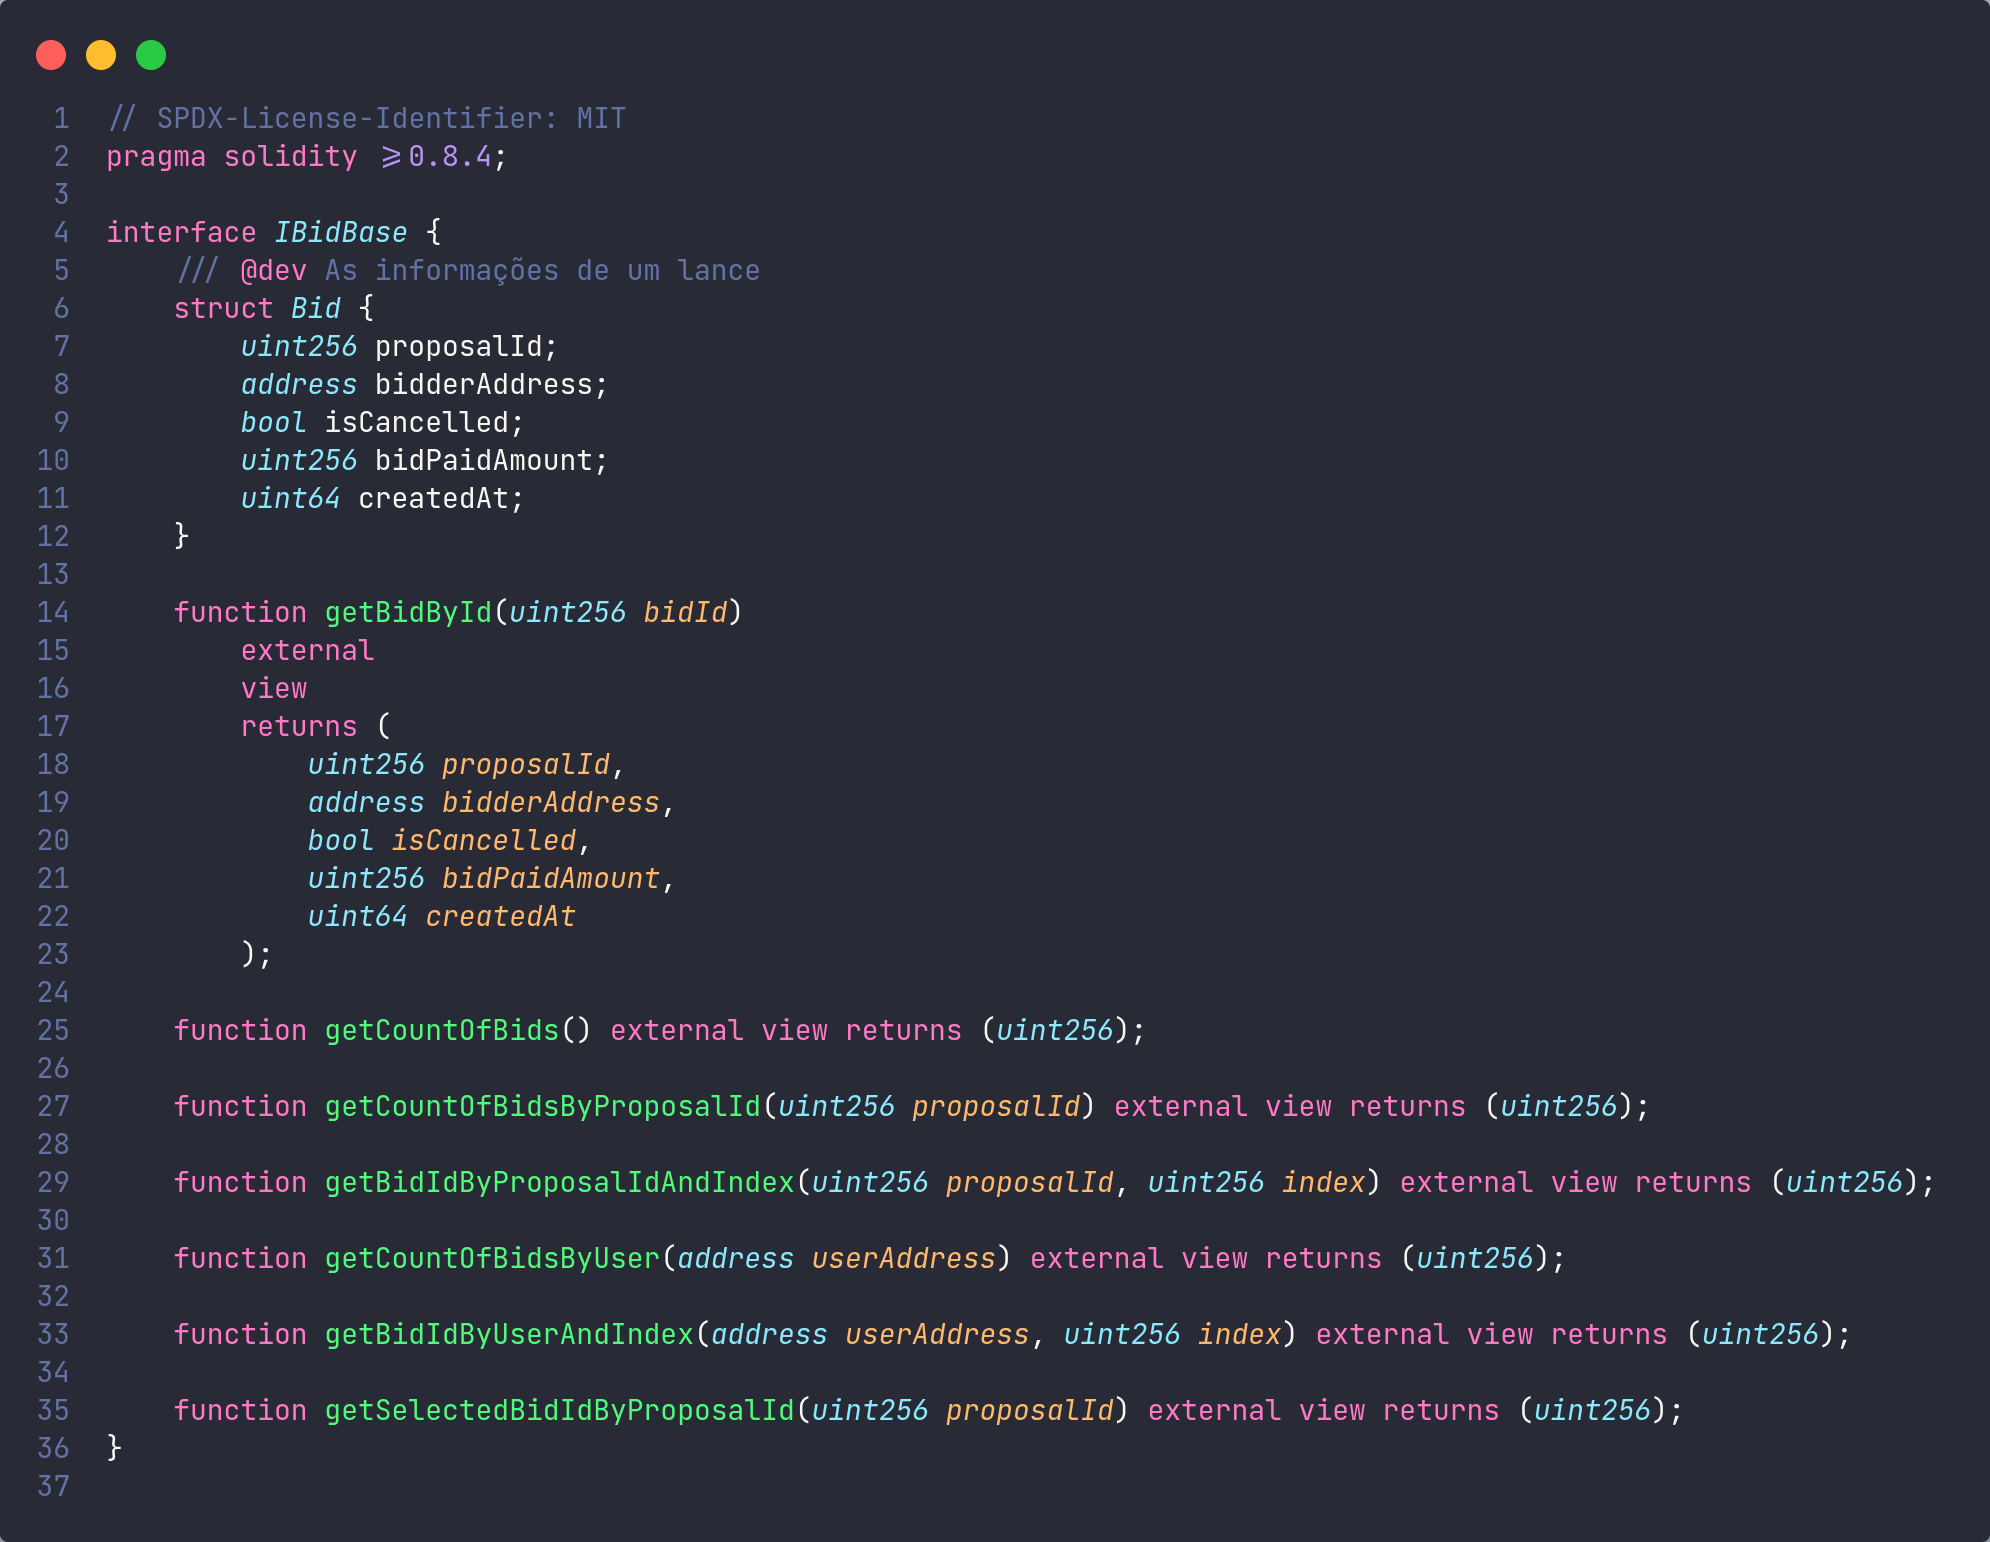
\includegraphics[width=420px]{src/images/contracts/bid_base.png}
  \subcaption{Fonte: Autor }
  \label{fig:bid_base_contract_fig}
\end{figure}

Pode-se observar que na figura \ref{fig:bid_base_contract_fig}, o contrato \textit{IBidBase} tem os métodos como \textit{getBidById} e \textit{getCountOfBids} para que o usuário possa listar todos os lances criados no contrato.

Além disso, há alguns métodos a mais que foram criados para que se possa integrar com as telas planejadas, como listar os lances de um usuário ou mesmo verificar qual lance foi selecionado para uma proposta.

E por fim, não foi criado uma interface para o contrato de \textit{BidProposal} porque esse contrato apenas expõe alguns métodos internos com a intenção de ser usado pelos métodos implementados das interfaces de \textit{IBidCore}.

Para ilustrar o propósito do contrato do \textit{BidProposal}, a figura \ref{fig:bid_proposal_fig} mostra o construtor do contrato e um dos métodos.

\begin{figure}[!h]
  \centering
  \caption{Contrato de Lances e Propostas}
  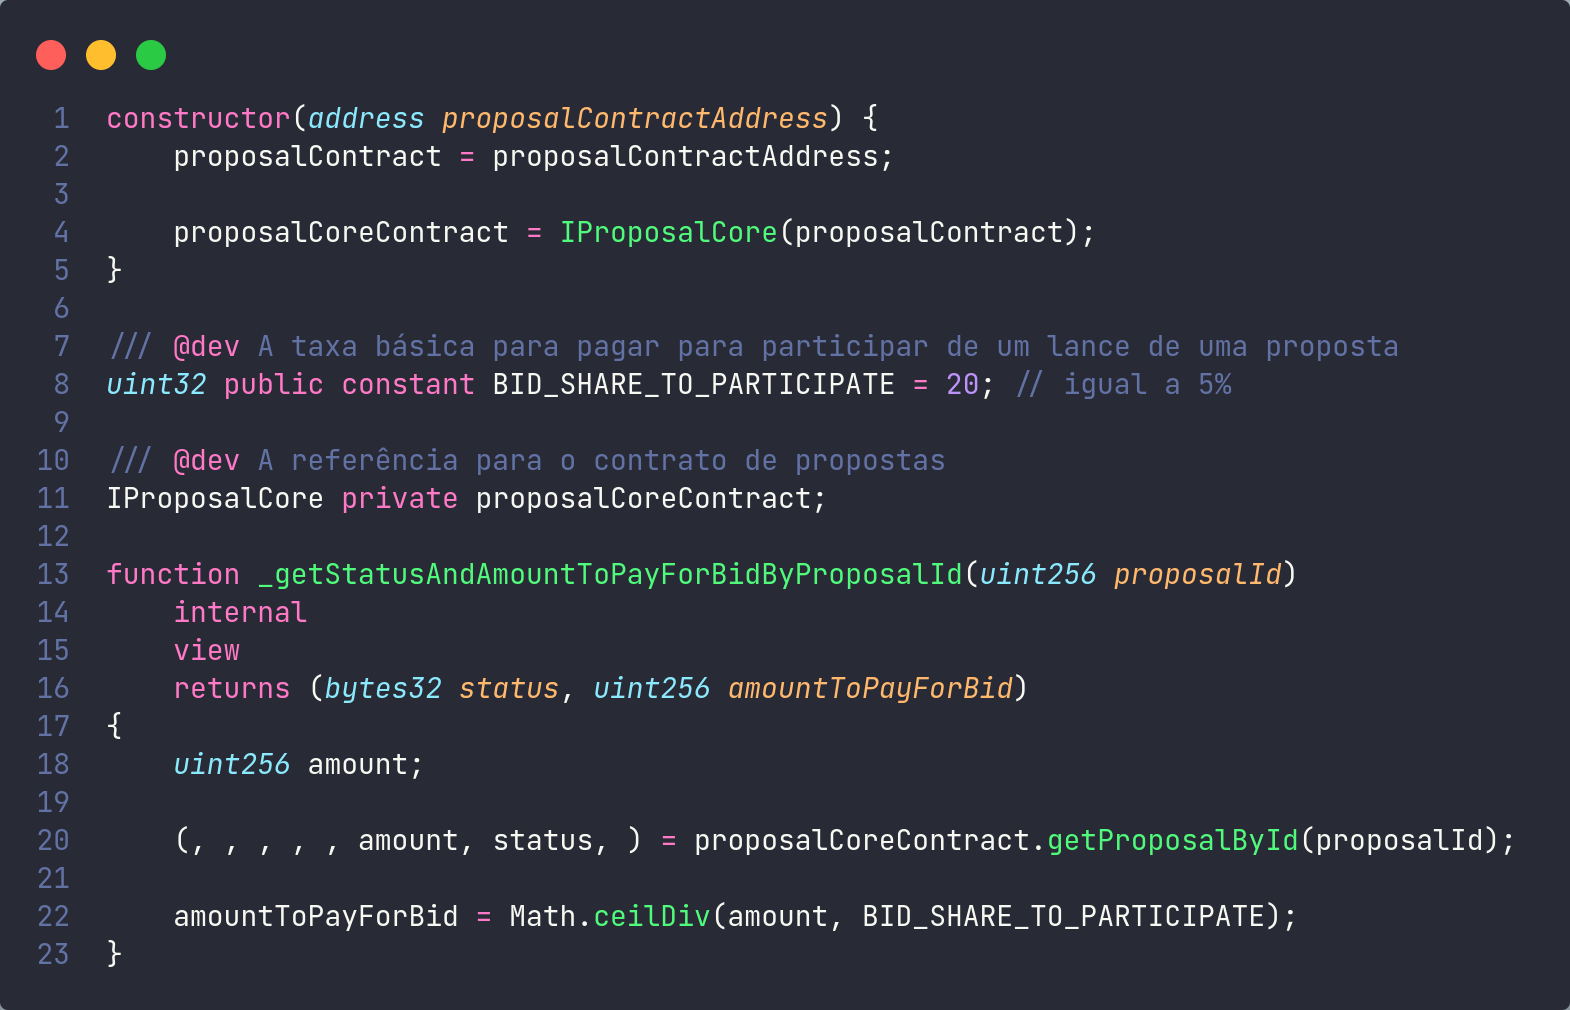
\includegraphics[width=420px]{src/images/contracts/bid_proposal.png}
  \subcaption{Fonte: Autor }
  \label{fig:bid_proposal_fig}
\end{figure}

Na linha 1 da figura \ref{fig:bid_proposal_fig}, o contrato irá receber o endereço do contrato de propostas, para que quando houver uma comunicação, seja assegurado que será do contrato de propostas correto. 

Há também uma constante chamada \textit{BID\_SHARE\_TO\_PARTICIPATE} que basicamente é usada para representar a porcentagem de quanto deve ser pago sobre o valor da proposta para que um lance seja criado. Essa constante é usada na linha 22 da figura \ref{fig:bid_proposal_fig}, no método que retorna o cálculo de quanto deve ser pago para criar um lance, assim como, saber o status da proposta.

\subsection{Disputas}

Para as disputas, foi divido em 2 interfaces e mais dois outros contratos que auxiliam a parte da comunicação com Lances e Propostas. As interfaces são \textit{IDisputeCore} e \textit{IDisputeBase}, junto dos contratos \textit{DisputeBid} e \textit{DisputeProposal}, responsáveis pela operações principais, operações básicas, comunicação com lances e comunicação com propostas, respectivamente.

A seguir, na figura \ref{fig:dispute_core_fig} será apresentado a interface \textit{IDisputeCore} que é usada para as operações principais.

\begin{figure}[!h]
  \centering
  \caption{Interface do contrato Core de Disputas}
  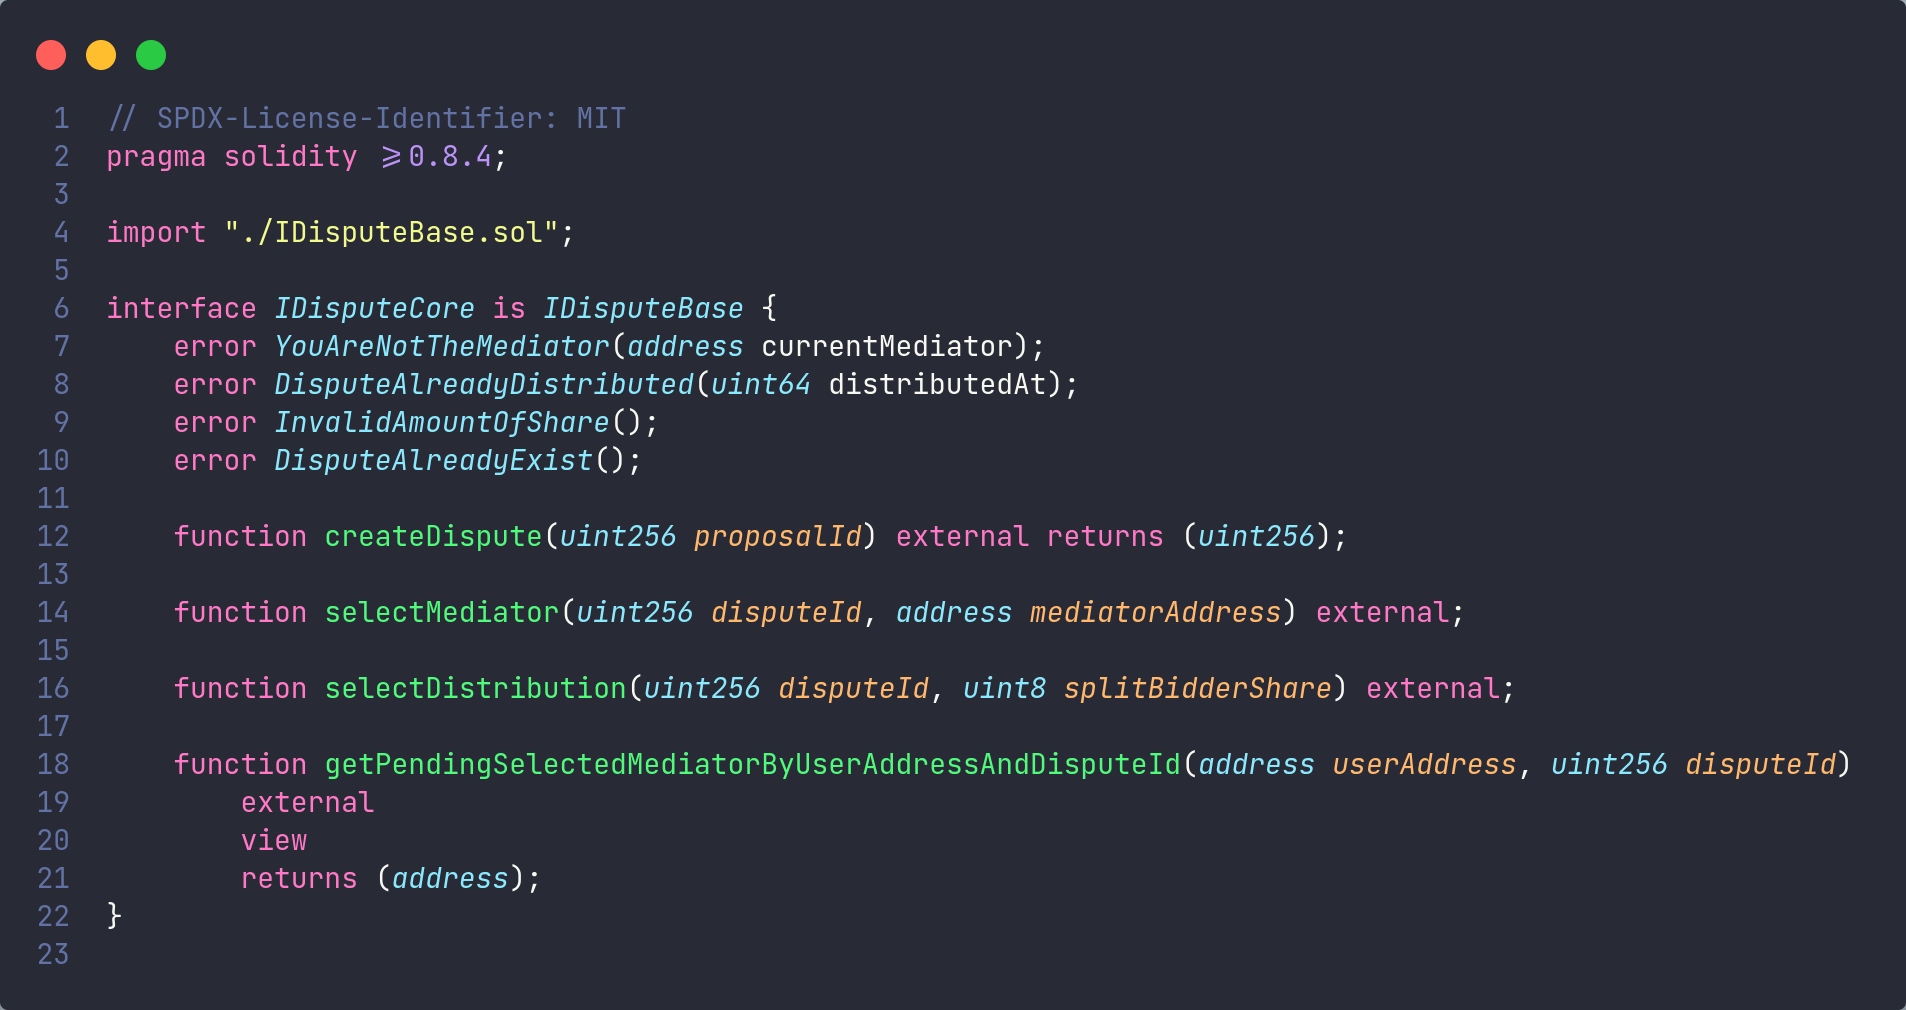
\includegraphics[width=420px]{src/images/contracts/dispute_core.png}
  \subcaption{Fonte: Autor }
  \label{fig:dispute_core_fig}
\end{figure}

Pode-se observar os métodos \textit{createDispute}, que é responsável pela criação de uma disputa, além de também notificar o contrato de proposta para atualizar o status da proposta.

Para as operações básicas, a figura \ref{fig:dispute_base_fig} mostra os métodos que são usados para listar as disputas, assim como mencionado anteriormente em propostas e lances, a combinação dos métodos de contar e buscar o item específico, no caso de disputa, \textit{getCountOfDisputes} e \textit{getDisputeById}.

\begin{figure}[!h]
  \centering
  \caption{Interface do contrato Base de Disputas}
  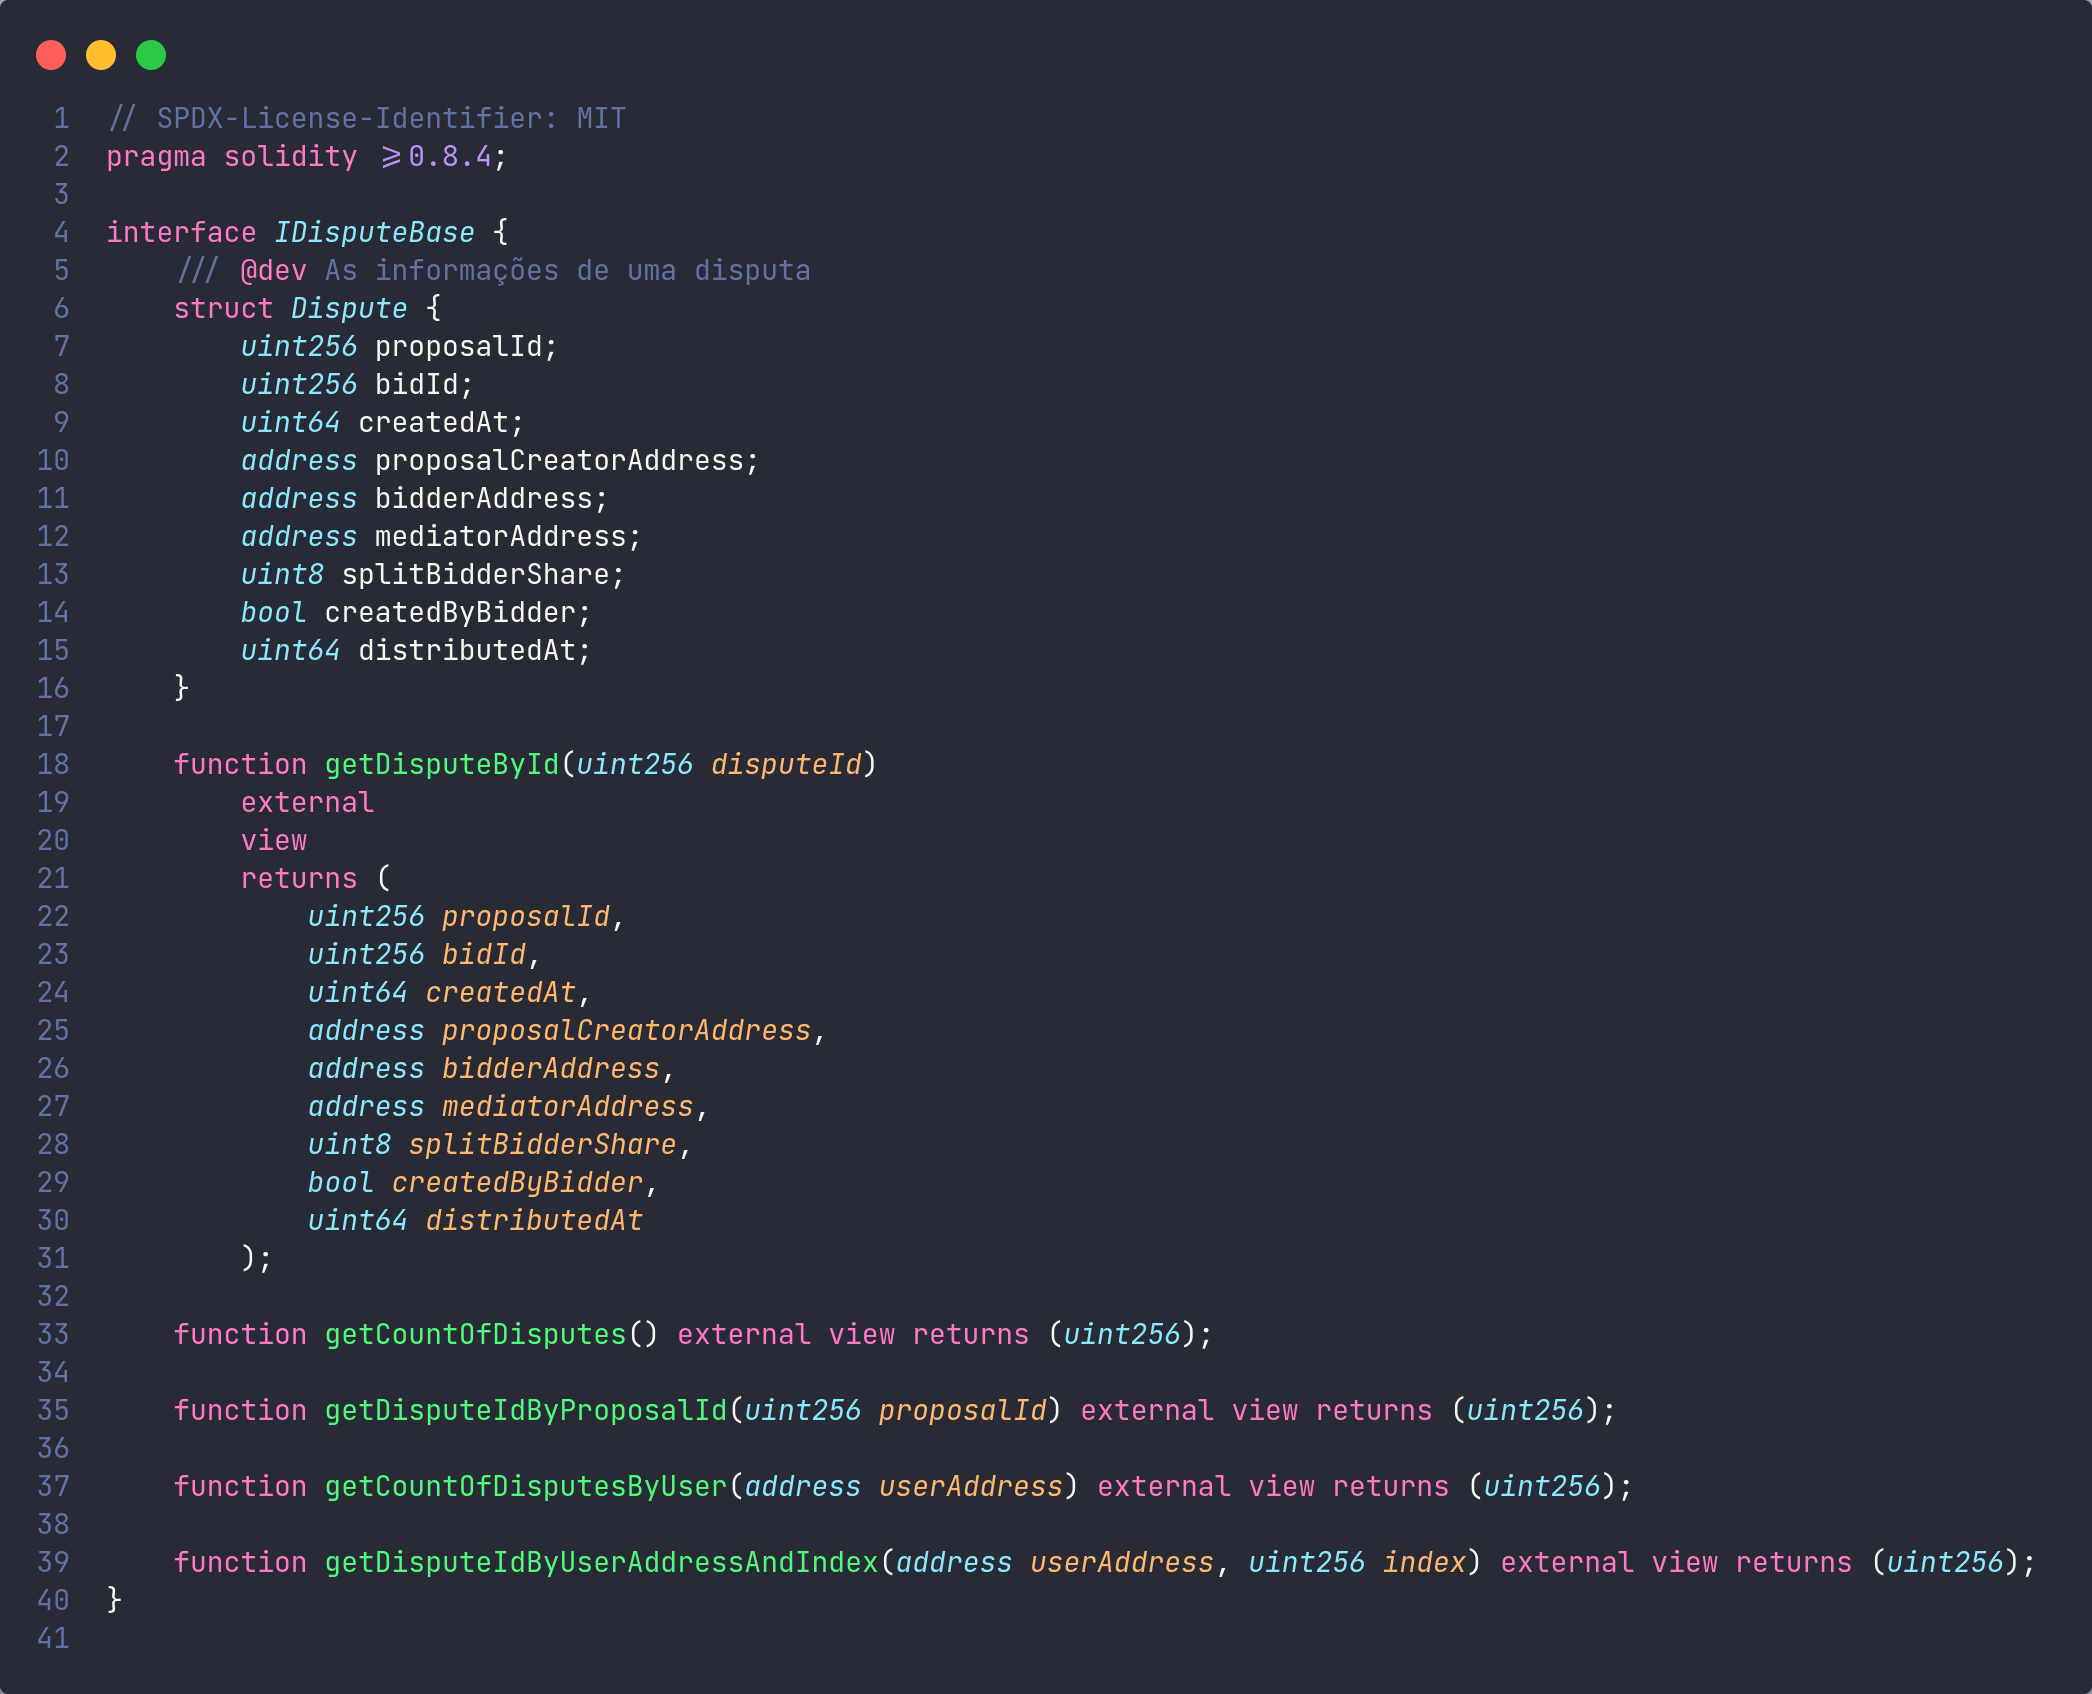
\includegraphics[width=360px]{src/images/contracts/dispute_base.png}
  \subcaption{Fonte: Autor }
  \label{fig:dispute_base_fig}
\end{figure}

Por fim, os dois contratos auxiliares, \textit{DisputeBid} e \textit{DisputeProposal} são exibidos nas figuras \ref{fig:dispute_bid_fig} e \ref{fig:dispute_proposal_fig}, respectivamente.

\begin{figure}[!h]
  \centering
  \caption{Contrato de Disputa e Lances}
  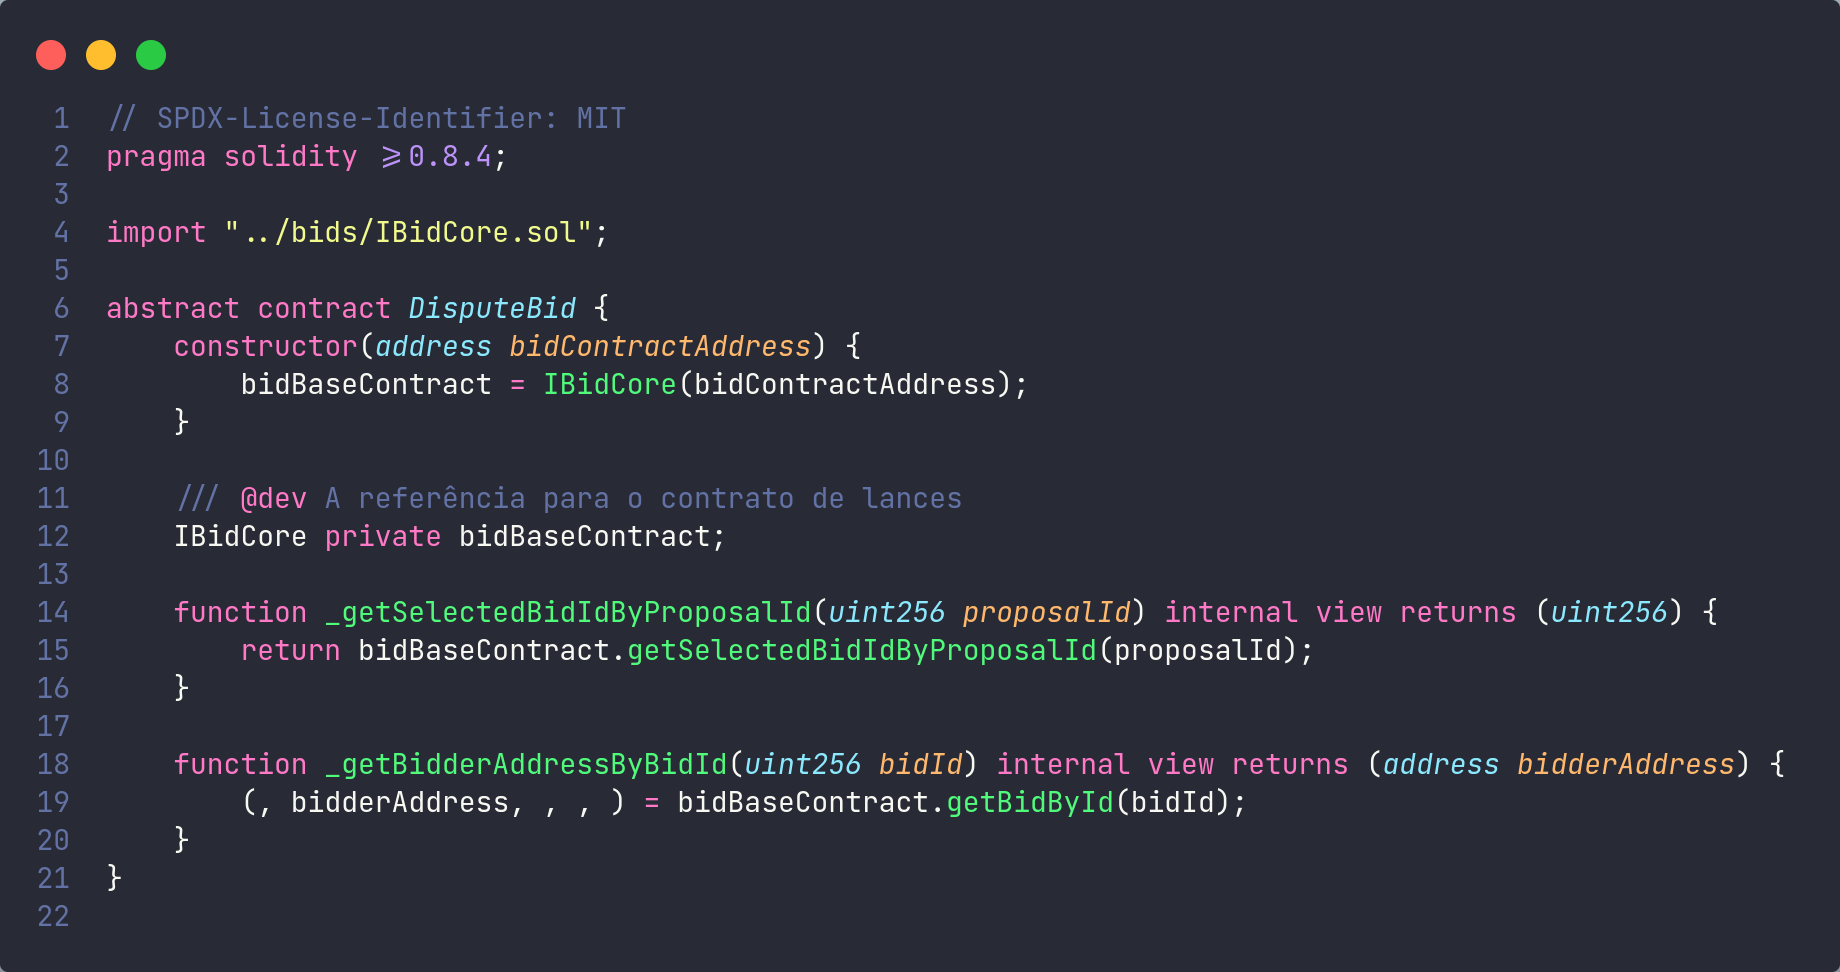
\includegraphics[width=400px]{src/images/contracts/dispute_bid.png}
  \subcaption{Fonte: Autor }
  \label{fig:dispute_bid_fig}
\end{figure}

\begin{figure}[!h]
  \centering
  \caption{Contrato de Disputa e Propostas}
  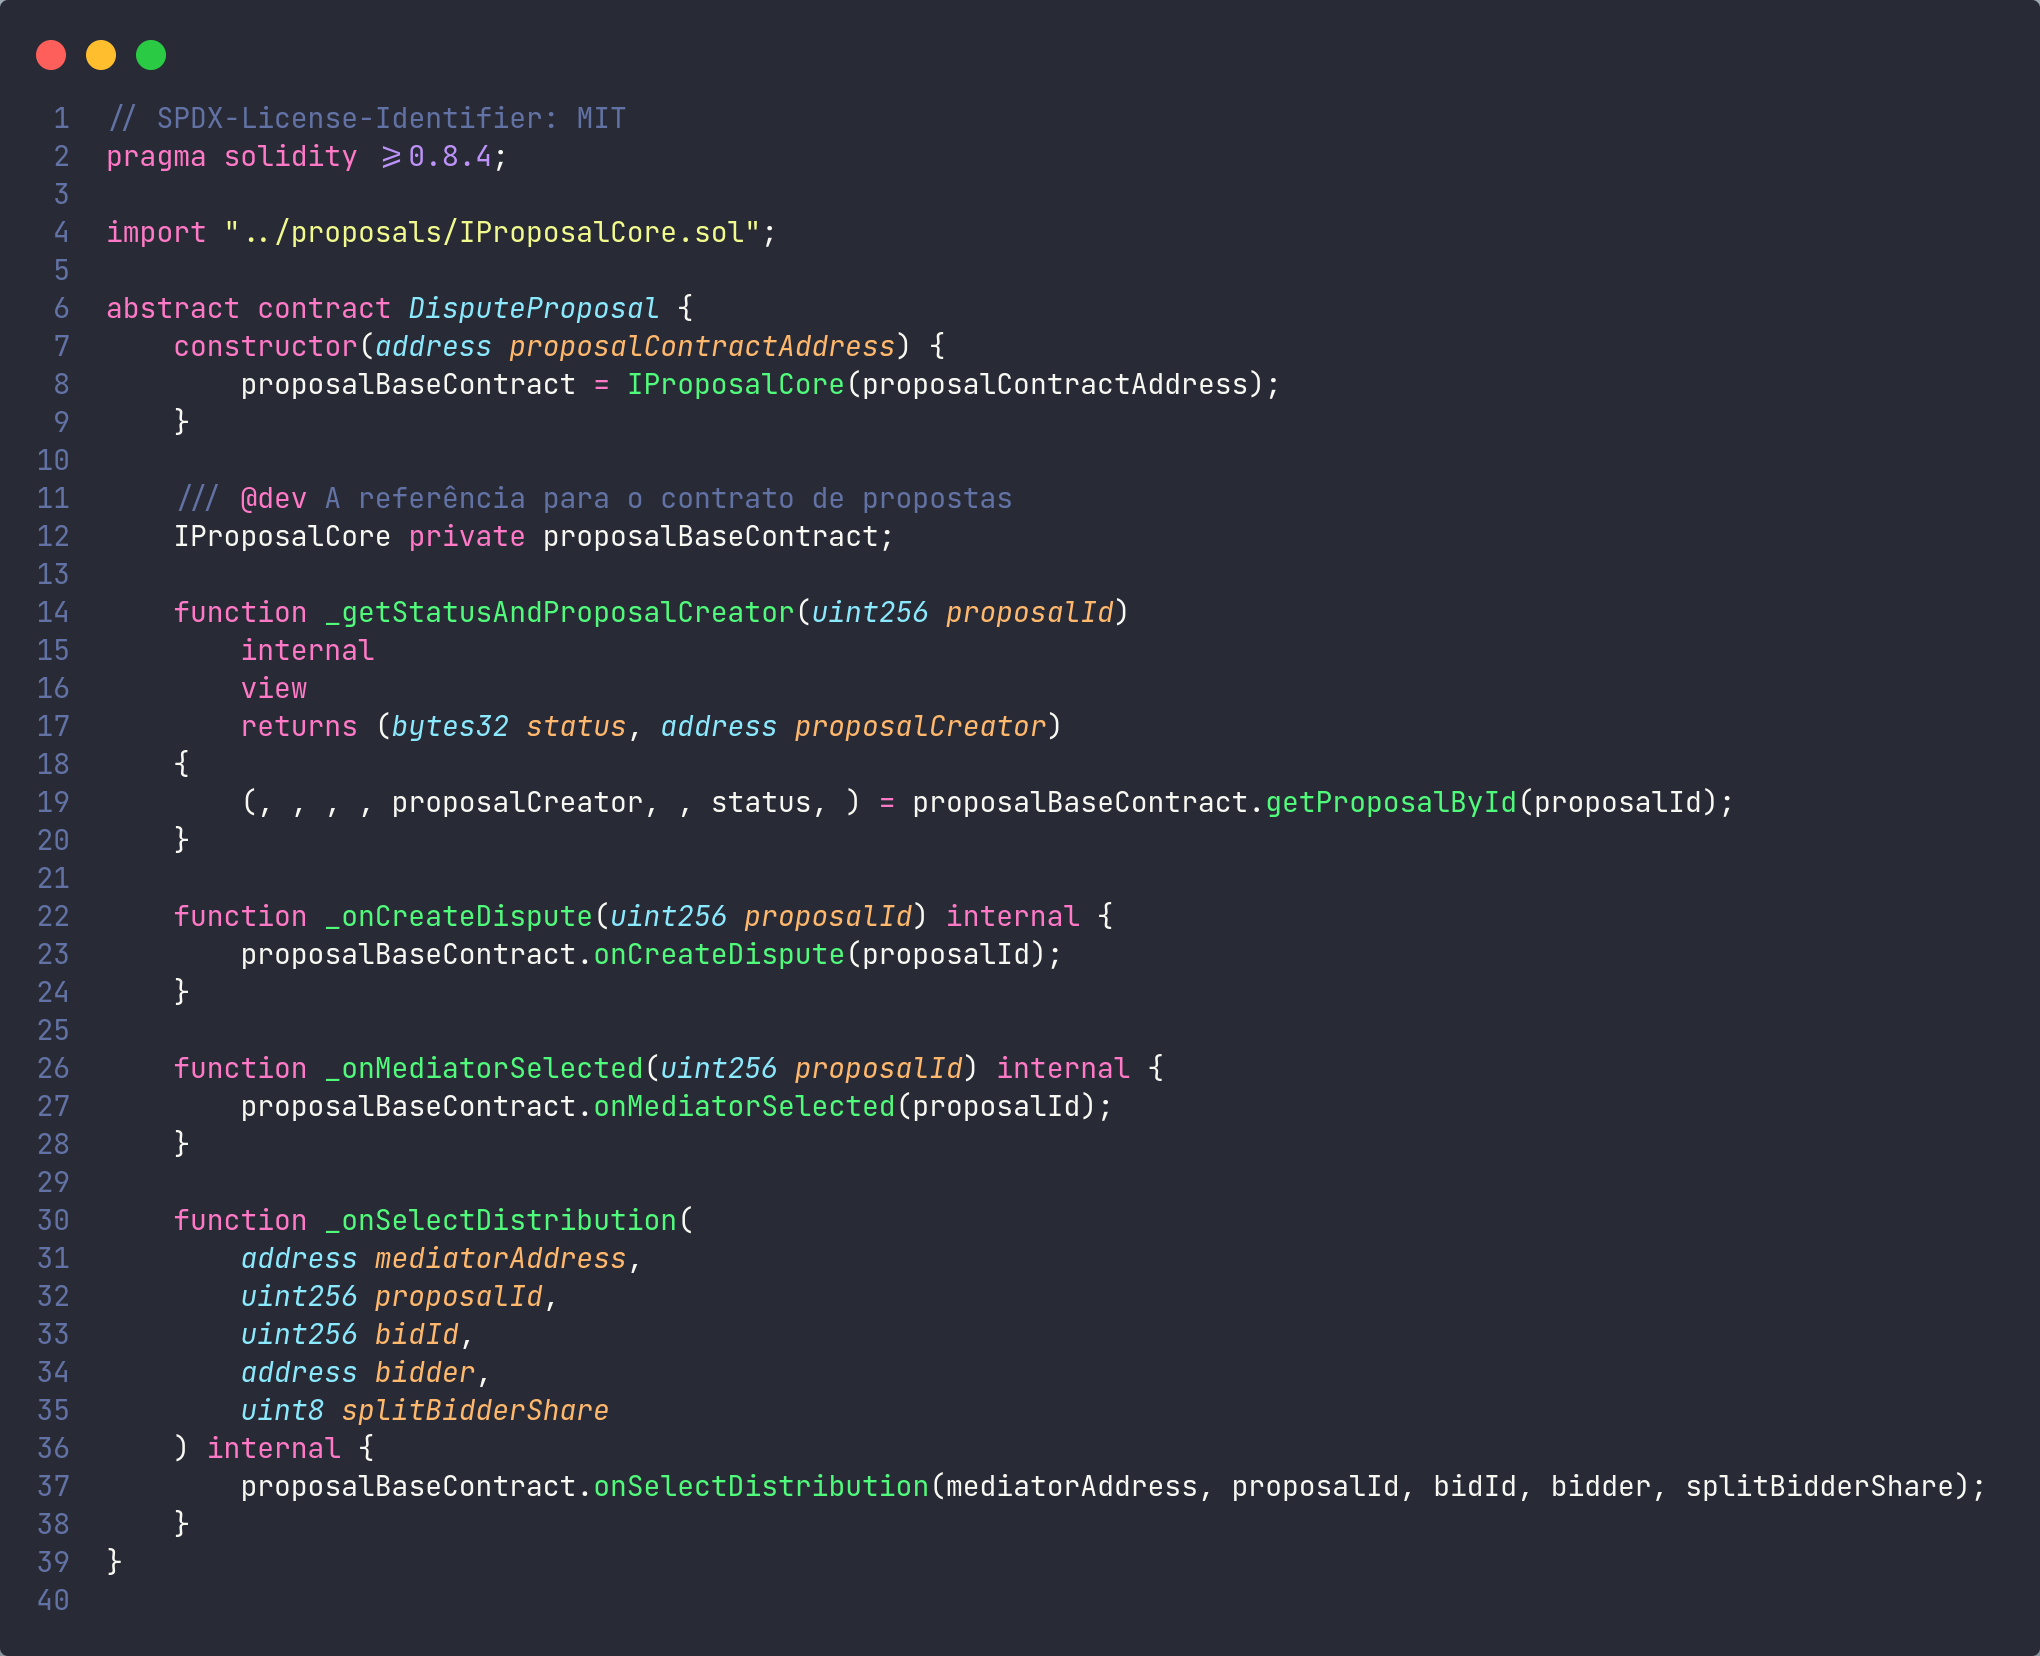
\includegraphics[width=350px]{src/images/contracts/dispute_proposal.png}
  \subcaption{Fonte: Autor }
  \label{fig:dispute_proposal_fig}
\end{figure}

Em ambos os contratos, as funções são principalmente para buscar o status da proposta, ou chamar os métodos de outros contratos para dizer que uma disputa foi criada, ou um mediador foi selecionado e até mesmo para transferir o valor dos contratos para quem o mediador preferiu.

Adentrando em mais especificidades dos contratos de disputa, é interessante analisar a implementação do método de \textit{selectDistribution} na figura \ref{fig:select_distribution_dispute_fig}, que é chamado pelo mediador para dividir os valores da proposta durante uma disputa.

\begin{figure}[!h]
  \centering
  \caption{Código do método de selectDistribution}
  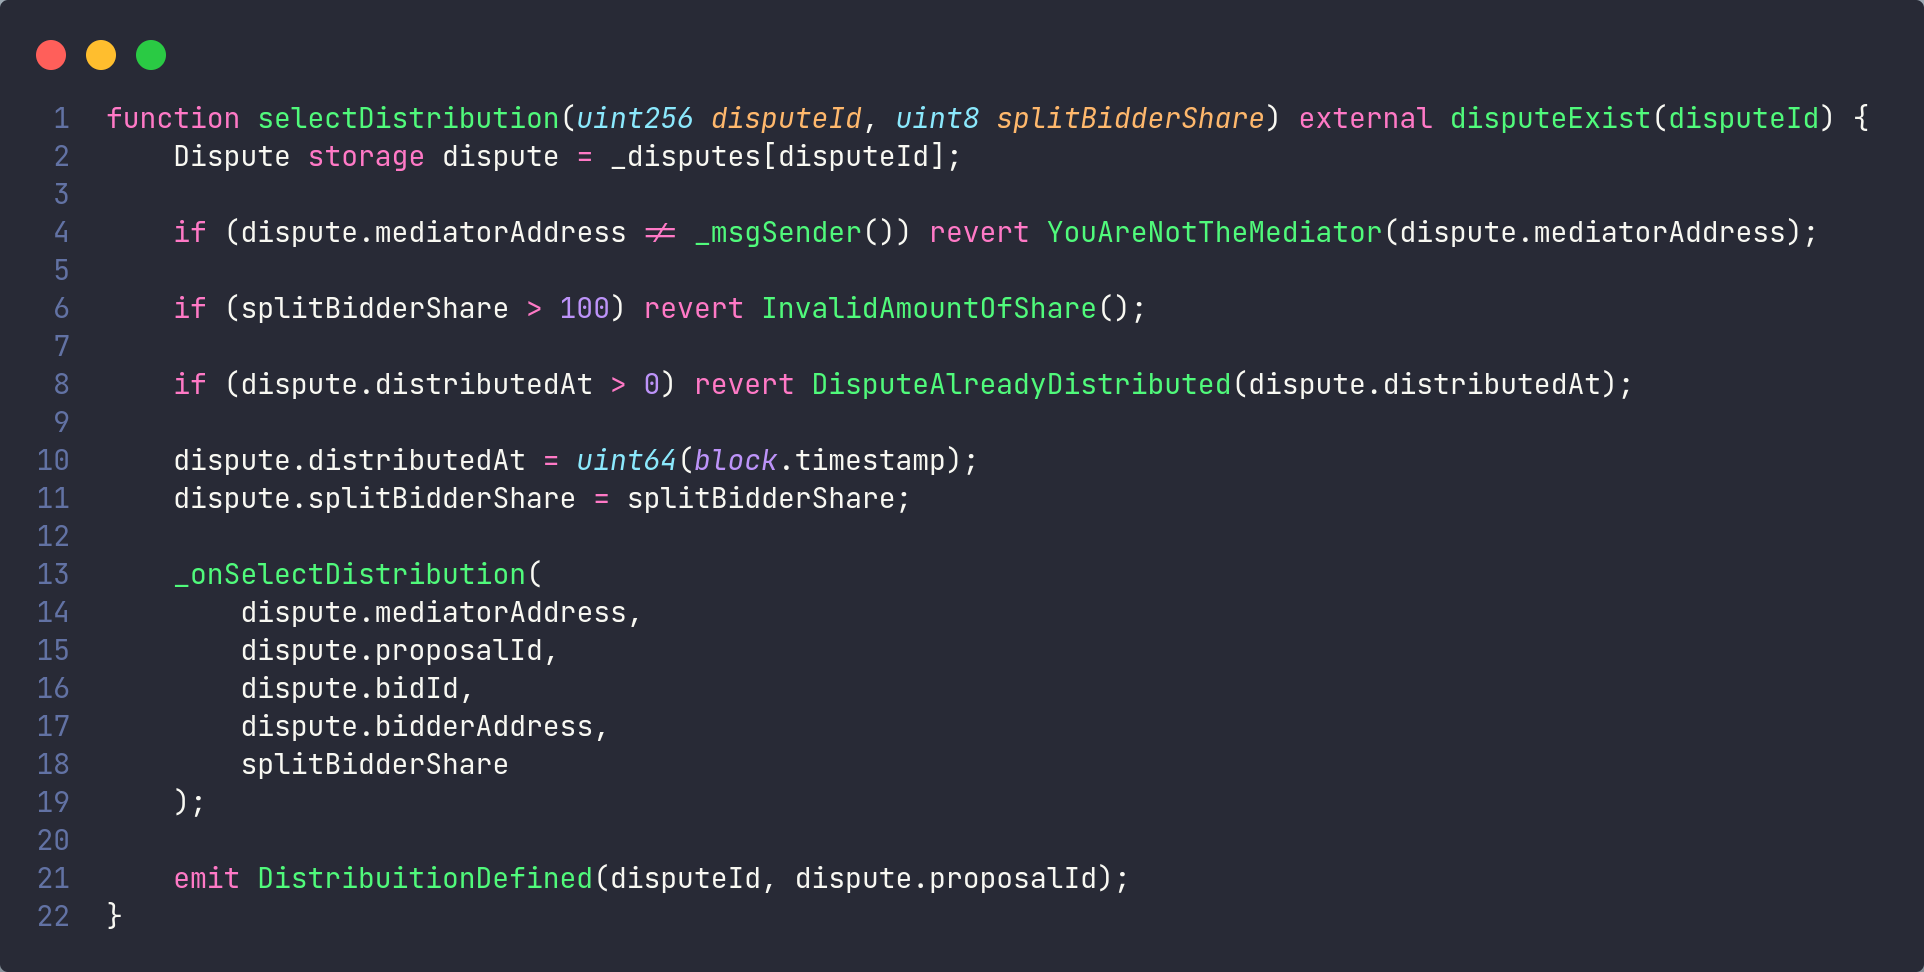
\includegraphics[width=400px]{src/images/contracts/select_distribution_dispute.png}
  \subcaption{Fonte: Autor }
  \label{fig:select_distribution_dispute_fig}
\end{figure}

Dentro desse método, ao analisar os quesitos de segurança, temos que na linha 8 da figura \ref{fig:select_distribution_dispute_fig} há uma validação para verificar se já foi distribuído os valores, e em seguida, na linha 10, é definido um valor para essa variável para que não permita que esse método seja chamado duas vezes.

Além disso, o método \textit{\_onSelectDistribution} é chamado para notificar os contratos de lance, que por sua vez, chama o contrato de propostas. A implementação no contrato de propostas pode ser observado na figura \ref{fig:on_select_distribution_proposal_fig}.

\begin{figure}[!h]
  \centering
  \caption{Código do método onSelectDistribution em propostas}
  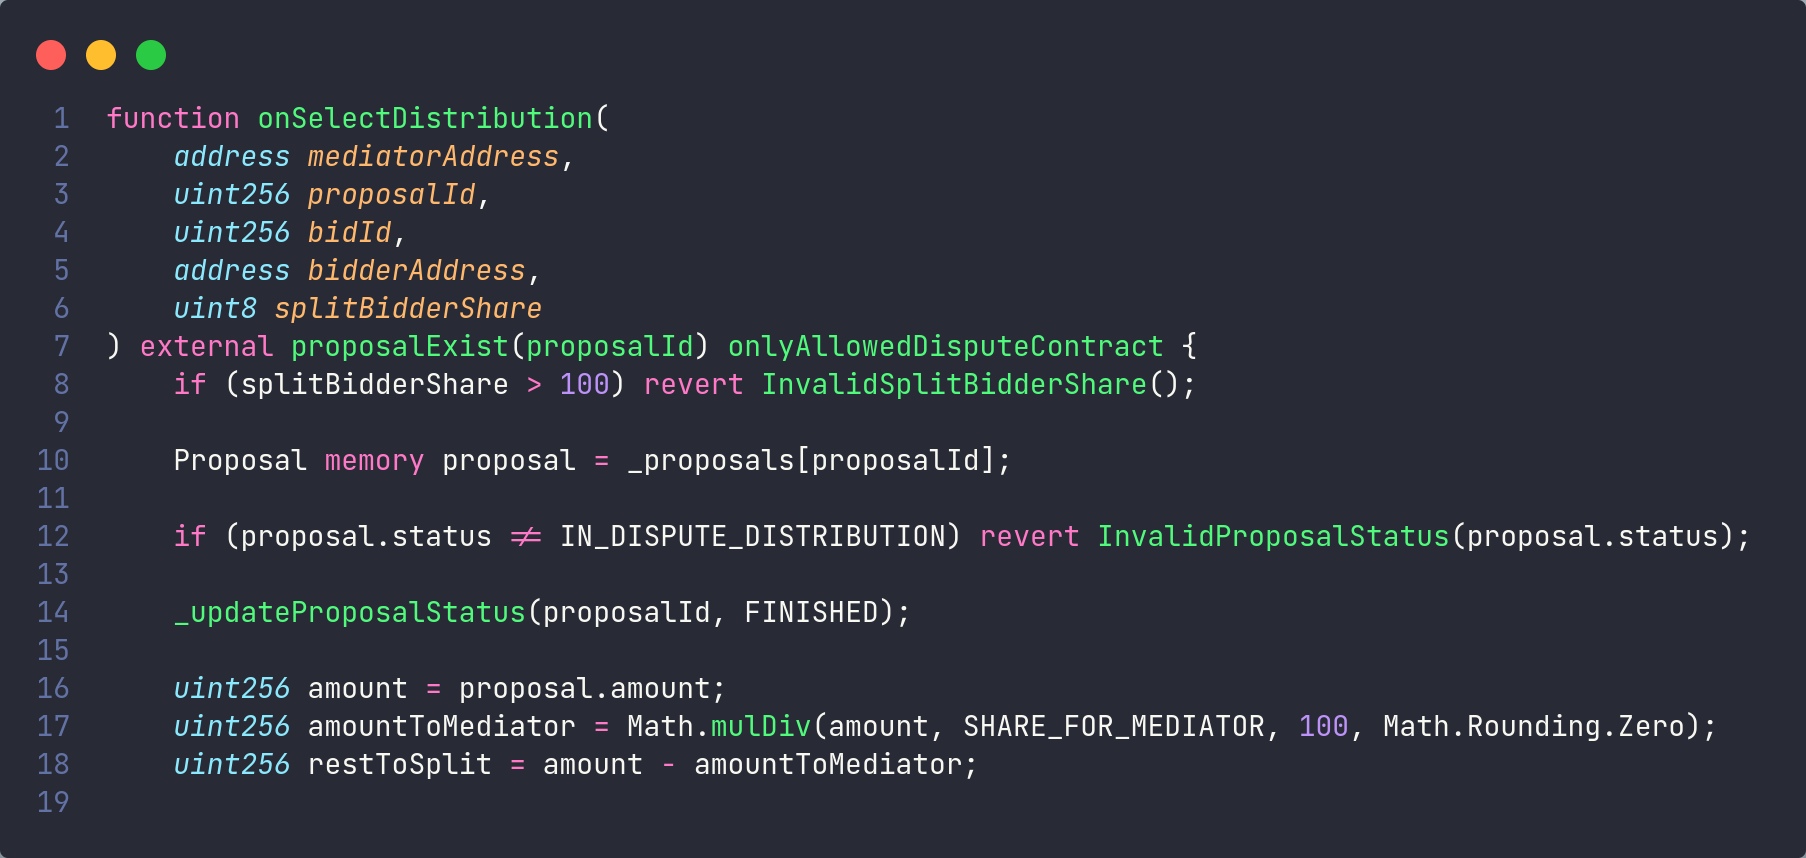
\includegraphics[width=320px]{src/images/contracts/on_select_distribution_proposal.png}
  \subcaption{Fonte: Autor }
  \label{fig:on_select_distribution_proposal_fig}
\end{figure}

Nas linhas 12 e 14 da figura \ref{fig:on_select_distribution_proposal_fig} há uma validação de segurança, e após isso, nas linhas 17 e 18 é calculado qual é o valor que será enviado para o mediador - 5\% do valor total da proposta - e o resto é divido de acordo com o que o mediador especificou. 

\subsection{Testes}

Para saber se o código escrito realmente fazia o que foi pretendido, foi escrito cerca de 71 testes no total para que fosse obtido uma cobertura de testes de 100\%. 
% A seguir, as figuras (\ref{fig:tests_proposal_fig}), (\ref{fig:tests_bid_fig}) e (\ref{fig:tests_dispute_fig}) representam, respectivamente, os testes dos contratos de Proposta, Lances e Disputa.
A seguir, na figura \ref{fig:tests_proposal_fig} é mostrado os testes criados para o contrato de proposta.

\begin{figure}[!h]
  \centering
  \caption{Testes do contrato de proposta}
  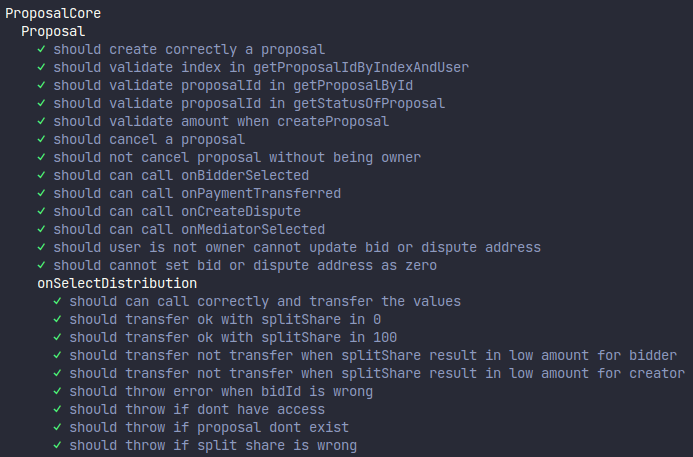
\includegraphics[width=400px]{src/images/contracts/tests_proposal.png}
  \subcaption{Fonte: Autor }
  \label{fig:tests_proposal_fig}
\end{figure}

É importante notar que foi criado sub-categorias nos testes para os métodos que realizam uma operação dentro do contrato de proposta, e para os métodos de visualização, os testes para eles são feitos durante os testes principais.

Após os testes de propostas, há os testes do contrato de disputa, que pode ser observado na figura \ref{fig:tests_bid_fig}.

\begin{figure}[!h]
  \centering
  \caption{Testes do contrato de lances}
  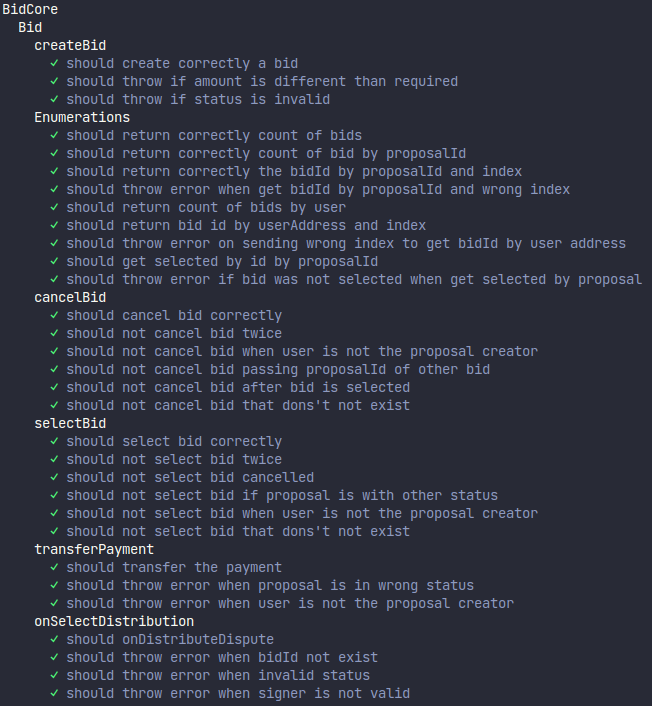
\includegraphics[width=320px]{src/images/contracts/tests_bid.png}
  \subcaption{Fonte: Autor }
  \label{fig:tests_bid_fig}
\end{figure}

E assim como no contrato de proposta, o foco dos testes do contrato de lances é testar os métodos que modificam o estado da \textit{Blockchain}. Além disso, o contrato de Lances é o que possui a maior quantidade de testes devido a quantidade a complexidade de suas operações.

E por fim, na figura \ref{fig:tests_dispute_fig} pode-se observar os testes escritos para o contrato de disputa, no qual o foco está em testar os métodos principais de criação de disputa, selecionar mediador e realizar a distribuição dos valores da proposta.

\begin{figure}[!h]
  \centering
  \caption{Testes do contrato de disputas}
  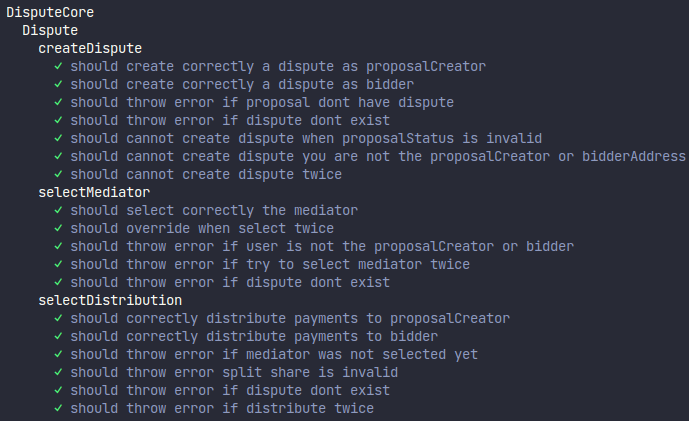
\includegraphics[width=320px]{src/images/contracts/tests_dispute.png}
  \subcaption{Fonte: Autor }
  \label{fig:tests_dispute_fig}
\end{figure}

Dessa forma, com os testes feitos, pode-se ter uma segurança maior que, o que foi proposto no desenvolvimento, será executado corretamente. Além disso, na figura \ref{fig:tests_coverage_fig}, há cobertura dos testes desenvolvidos.

\begin{figure}[!h]
  \centering
  \caption{Testes do contrato de proposta}
  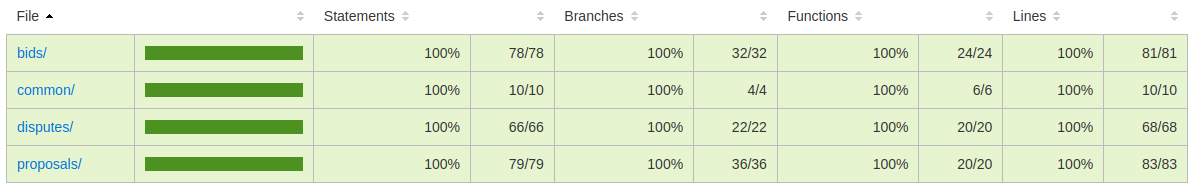
\includegraphics[width=450px]{src/images/contracts/tests_coverage.png}
  \subcaption{Fonte: Autor }
  \label{fig:tests_coverage_fig}
\end{figure}

E conforme pode ser observado na figura \ref{fig:tests_coverage_fig}, tanto as linhas quanto as \textit{branches} estão em 100\%, que significa todas as ramificações e caminhos possíveis no código estão com uma cobertura completa.

\subsection{Consumo de \texit{Gas}}

Um fator importante para a viabilidade da plataforma é saber o quanto de \textit{Gas} cada operação que modifica o estado da \textit{Blockchain} está consumindo. A seguir, é mostrado na tabela \ref{tab:report_gas} o consumo médio de cada método por contrato.

\begin{table}[!h]
\centering
\caption{Consumo de Gas por método}
\label{tab:report_gas}
\begin{tabular}{@{}lll@{}}
\toprule
Contrato & Método    & Média (gas) \\ \midrule
Proposta & cancelProposal & 55416 \\
Proposta & createProposal & 301054 \\
Proposta & onBidderSelected & 50589 \\
Proposta & onCreateDispute & 50512 \\
Proposta & onMediatorSelected & 50457 \\
Proposta & onPaymentTransferred & 60541 \\
Proposta & onSelectDistribution & 108538 \\
Proposta & setBidContractAddress & 42251 \\
Proposta & setDisputeContractAddress & 31531 \\
Lance & cancelBid & 44540 \\
Lance & createBid & 296738 \\
Lance & onSelectDistribution & 72834 \\
Lance & selectBid & 99942 \\
Lance & transferPayment & 91653 \\
Dispute & createDispute & 373572 \\
Dispute & selectDistribution & 126345 \\
Dispute & selectMediator & 73402 \\ \bottomrule
\end{tabular}
\begin{tablenotes}
  \small
  \item Fonte: Autor
\end{tablenotes}
\end{table}

Além do consumo por método, foi medido também o consumo de \textit{Gas} para hospedar o contrato na rede \textit{Blockchain}, esse consumo é mostrado na tabela \ref{tab:report_gas_contract}.

\begin{table}[!h]
\centering
\caption{Consumo de Gas por contrato}
\label{tab:report_gas_contract}
\begin{tabular}{@{}lll@{}}
\toprule
Contrato    & Média (gas) \\ \midrule
Proposta  & 1372426 \\
Lance     & 1236650 \\
Disputa   & 2495562 \\ \bottomrule
\end{tabular}
\begin{tablenotes}
  \small
  \item Fonte: Autor
\end{tablenotes}
\end{table}

O consumo do contrato é calculado pela quantidade de código - também chamado por \textit{bytecode} - resultante da compilação do contrato. Para entender melhor a quantidade de \textit{Gas}, veja a tabela \ref{tab:report_contract_size} para verificar o tamanho do contrato em bytes.

\begin{table}[!h]
\centering
\caption{Tamanho em bytes por contrato}
\label{tab:report_contract_size}
\begin{tabular}{@{}lll@{}}
\toprule
Contrato  & Tamanho (KiB) \\ \midrule
Proposta  & 10,931 \\
Lance     & 5,641 \\
Disputa   & 5,021 \\ \bottomrule
\end{tabular}
\begin{tablenotes}
  \small
  \item Fonte: Autor
\end{tablenotes}
\end{table}

Para ter uma comparação, o tamanho máximo permitido para um contrato, segundo EIP 170, é definido como 24KiB. Até pode parecer bastante mas dependendo de que tipo de operação você escolhe e como organizar os contratos, o tamanho pode realmente se aproximar facilmente do limite. E ao atingir esse limite, a única escolha é dividir o contrato ou buscar otimizar o contrato.

Por fim, para dar contexto ao consumo de \textit{Gas}, é necessário calcular a taxa de cada operação através da taxa base em \textit{Gwei}, que é a menor unidade da moeda de um \textit{Ether} ou \textit{Matic}, multiplicado pelo \textit{Gas} usado. Dessa forma, na tabela \ref{tab:report_gwei_price}, é mostrado a taxa base em \textit{Gwei} na rede no qual foi feito a hospedagem dos contratos (\textit{Polygon}), assim como, na rede \textit{Ethereum} para ter uma comparação, por data.

\begin{table}[!h]
\centering
\caption{Taxa base na Ethereum e Polygon}
\label{tab:report_gwei_price}
\begin{tabular}{@{}lll@{}}
\toprule
Data  & Ethereum (Gwei) & Polygon (Gwei) \\ \midrule
01/09/2019  & 14,73 & Sem dados \\ 
01/05/2022  & 60,05 & 90,26 \\ 
01/10/2022  & 11,41 & 154,21 \\ \bottomrule
\end{tabular}
\begin{tablenotes}
  \small
  \item Fonte: \cite{ethereum_gwei_price} e \cite{polygon_gwei_price}
\end{tablenotes}
\end{table}

Com a taxa base, é necessário entender quanto custa cada \textit{Gwei} consumido, para que, ao ter o valor multiplicado, seja possível obter o valor de cada operação em R\$. Dessa forma, na tabela \ref{tab:report_gwei_to_real} é mostrado o preço de cada \texit{Gwei} em reais.

\begin{table}[!h]
\centering
\caption{Preço de um Gwei na Ethereum e Polygon}
\label{tab:report_gwei_to_real}
\begin{tabular}{@{}lll@{}}
\toprule
Data  & Ethereum (R\$) & Polygon (R\$) \\ \midrule
01/09/2019  & 1424,87 & Sem dados \\ 
01/05/2022  & 14551,91 & 5,66 \\ 
01/10/2022  & 6772,92 & 3,98 \\ \bottomrule
\end{tabular}
\begin{tablenotes}
  \small
  \item Fonte: \cite{ethereum_price_2019}, \cite{ethereum_price_2022} e \cite{ethereum_price_10_2022} convertido usando 5,16370 REAL/USD corrigido pela inflação do período. \cite{inflation_calculator}.
\end{tablenotes}
\end{table}

Pode-se observar, na tabela \ref{tab:report_gwei_to_real}, que em 2019 não há dados para a \textit{Polygon}, isso acontece porque ela só foi lançada em 2020.

Por fim, usando a referência que 1 ether que é igual a \(10^9\) Gwei, usando os custos da taxa e o preço de cada moeda, o preço da taxa de cada operação na rede \texit{Ethereum} foi calculado e representado na tabela \ref{tab:report_prices_per_method_ethereum}, e para a rede Polygon na tabela \ref{tab:report_prices_per_method_polygon}.

\begin{table}[!h]
\centering
\caption{Preço da taxa de cada operação na Ethereum}
\label{tab:report_prices_per_method_ethereum}
\begin{tabular}{@{}llll@{}}
\toprule
Método & 01/09/2019 (R\$) & 01/05/2022 (R\$) & 01/10/2022 (R\$) \\ \midrule
cancelProposal & 1,16 & 48,42 & 4,28 \\
createProposal & 6,32 & 263,07 & 23,27 \\
onBidderSelected & 1,06 & 44,21 & 3,91 \\
onCreateDispute & 1,06 & 44,14 & 3,90 \\
onMediatorSelected & 1,06 & 44,09 & 3,90 \\
onPaymentTransferred & 1,27 & 52,90 & 4,68 \\
onSelectDistribution & 2,28 & 94,85 & 8,39 \\
setBidContractAddress & 0,89 & 36,92 & 3,27 \\
setDisputeContractAddress & 0,66 & 27,55 & 2,44 \\
cancelBid & 0,93 & 38,92 & 3,44 \\
createBid & 6,23 & 259,30 & 22,93 \\
onSelectDistribution & 1,53 & 63,65 & 5,63 \\
selectBid & 2,10 & 87,33 & 7,72 \\
transferPayment & 1,92 & 80,09 & 7,08 \\
createDispute & 7,84 & 326,44 & 28,87 \\
selectDistribution & 2,65 & 110,41 & 9,76 \\
selectMediator & 1,54 & 64,14 & 5,67 \\ \bottomrule
\end{tabular}
\begin{tablenotes}
  \small
  \item Fonte: Autor
\end{tablenotes}
\end{table}

\begin{table}[!h]
\centering
\caption{Preço da taxa de cada operação na Polygon}
\label{tab:report_prices_per_method_polygon}
\begin{tabular}{@{}lll@{}}
\toprule
Método & 01/05/2022 (R\$) & 01/10/2022 (R\$) \\ \midrule
cancelProposal & 0,03 & 0,03 \\
createProposal & 0,15 & 0,18 \\
onBidderSelected & 0,03 & 0,03 \\
onCreateDispute & 0,03 & 0,03 \\
onMediatorSelected & 0,03 & 0,03 \\
onPaymentTransferred & 0,03 & 0,04 \\
onSelectDistribution & 0,06 & 0,07 \\
setBidContractAddress & 0,02 & 0,03 \\
setDisputeContractAddress & 0,02 & 0,02 \\
cancelBid & 0,02 & 0,03 \\
createBid & 0,15 & 0,18 \\
onSelectDistribution & 0,04 & 0,04 \\
selectBid & 0,05 & 0,06 \\
transferPayment & 0,05 & 0,06 \\
createDispute & 0,19 & 0,23 \\
selectDistribution & 0,06 & 0,08 \\
selectMediator & 0,04 & 0,05 \\ \bottomrule
\end{tabular}
\begin{tablenotes}
  \small
  \item Fonte: Autor
\end{tablenotes}
\end{table}
\chapter{Análise de Resultados}

Pode-se observar em resultados o que foi produzido para o site e os \textit{Smart Contracts}, um total de 5 telas com diversos estados que se integram com 3 contratos diferentes.

Com o objetivo de criar uma plataforma de freelance descentralizada, a implementação com a \textit{Polygon} ocorreu sem nenhum problema, além disso, com os contratos escritos em \textit{Solidity}, pode-se no futuro hospedar os mesmos contratos na \textit{Ethereum} caso os custos sejam viáveis.

Quanto aos custos de se usar a plataforma, a decisão de optar pela \textit{Polygon} se mostrou muito boa, para criar uma proposta na \textit{Ethereum} custa R\$ 263,07 (01/05/2022) em comparação com os R\$ 0,15 (01/05/2022) da \textit{Polygon}. Contudo, os preços das taxas de transação são variáveis, por exemplo, o custo da criação de uma proposta na \textit{Ethereum} em 01/09/2019 e 01/10/2022 foi de, respectivamente, R\$ 6,32 e R\$ 23,27. Nessa faixa, tanto em 2019 quanto no mês 10/2022 faz-se necessário que o valor armazenado em uma proposta tenha que ser muito maior do que poderia ser, como no caso da rede da \textit{Polygon} com as taxas mais baixas.

E uma informação importante a se atentar, em 01/05/2022 a \textit{Ethereum} funcionava com o algoritmo de consenso chamado \textit{Proof-of-Work}, e em 01/10/2022, o algoritmo de consenso já havia sido alterado para o \textit{Proof-of-Stake}, causando uma redução nos custos das taxas de transação, e esse é o motivo do porque os custos da criação de proposta no exemplo anterior foi reduzido de R\$ 263,07 (01/05/2022) para R\$ 23,27 (01/10/2022). Apesar dessa mudança, os custos da rede \textit{Polygon} ainda estão muito abaixo dos custos da \textit{Ethereum}, o que é mais um indicador que a \textit{Polygon} consegue ser mais eficiente que a \textit{Ethereum} com relação a taxas de transação. 

Além disso, é necessário considerar que as taxas não estão apenas na criação da proposta, para um ciclo completo, considerando que tudo ocorra sem problemas de disputa, seria necessário chamar os métodos: \textit{createProposal}, \textit{createBid}, \textit{selectBid} e \textit{transferPayment}. Ao chamar esses métodos, as taxas pagas,  usando a data de 01/10/2022 como referência, ficam em R\$ 38,07 para o criador e R\$ 22,93 para o freelancer, desconsiderando a porcentagem de 5\% a ser pago pelo freelancer. Ao calcular as mesmas taxas usando a data de 01/10/2022 como referência na \textit{Polygon}, o valor fica R\$ 0,30 para o criador e R\$ 0,18 para o freelancer, o que é muito abaixo e viabiliza o projeto como um todo.

Ademais, é importante mencionar o tamanho dos contratos, foi optado por implementar todas as funcionalidades que o sistema poderia ter em três contratos diferentes para evitar que atingisse o limite de tamanho de contrato de 24KiB. Como pode ser observado na tabela \ref{tab:report_contract_size}, o contrato mais pesado, o de proposta, ficou em torno de 10,9 KiB. Dessa forma, é possível levar esse resultado como uma melhoria para um próximo trabalho, no qual os três contratos poderiam ser apenas um, visto que, o tamanho somado dos três contratos é 21,593 KiB e isso poderia trazer um custo de taxa bem menor por não haver comunicação entre contratos.

Na introdução, também foi mencionado a hospedagem do site utilizando a tecnologia \textit{IPFS}, que foi realizada com sucesso, sendo possível acessar os arquivos através das identificações na seção de resultados.
Contudo, é interessante notar que o sistema \textit{IPFS} não necessariamente armazena indefinidamente, ainda é necessário que, alguns servidores em algum lugar do mundo, armazenem essa informação. Todavia, pode ocorrer que todos esses servidores removam a página sem aviso prévio, como uma forma de liberar espaço ao remover conteúdos pouco acessados. 

Porém, há como contornar esse problema com a funcionalidade de \textit{PIN}, ou fixar, que basicamente é uma função que uma pessoa com algum servidor diz que os arquivos fixados nunca devem ser apagados, dessa forma, o criador da plataforma e seus usuários podem coordenar de ter alguns servidores com os arquivos do site fixados para que os arquivos não sejam apagados acidentalmente.

Ademais, não houve problemas durante o desenvolvimento do site em \textit{Angular}, que junto das bibliotecas \textit{ethers} e \textit{rxjs}, pode-se ter um site reativo, de forma que, todo a lógica de lidar com atualização de estado ao modificar uma proposta se tornou simples de gerenciar, apesar de utilizar conceitos avançados.

Por fim, é importante salientar que para hospedar os contratos dentro da \textit{Solidity}, é necessário criar uma conta na plataforma, e os contratos hospedados podem ser pausados caso o número de operações ultrapasse uma quantia fixa. Dessa forma, foi possível atingir um certo grau de descentralização através das tecnologias de \textit{Blockchain}, contudo, é possível que em um outro trabalho possa ser feito a hospedagem dos contratos criados na \textit{Ethereum} ou outra solução, visando um grau ainda maior de descentralização ao mesmo tempo que se compara os custos.

% resposta a nossa introdução e ligação direta com o resto do TCC

%fichacatalografica@facens.br


\chapter{Conclusão}

Esse trabalho começou com um objetivo de criar uma plataforma de \textit{Freelance} que fosse descentralizada, de forma que, qualquer pessoa pudesse usar de qualquer lugar do mundo. Esse objetivo foi atingido ao utilizar das mesmas tecnologias que compõem o \textit{Bitcoin} e a \textit{Ethereum}, duas soluções que é usado pelo mundo inteiro com alta disponibilidade e de livre acesso.

Ao optar por utilizar tecnologias que estão em constante evolução, foi possível observar evoluções enquanto esse trabalho estava sendo desenvolvido, como a mudança do algoritmo de consenso da \textit{Ethereum} descrito em fundamentos teóricos, visando a redução das taxas de transação. E apesar dessa constante evolução, foi possível criar uma solução que pode ser usada por qualquer pessoa a rede da \textit{Polygon}, em conjunto com tecnologias como \textit{IPFS} e \textit{Angular}.

Esse trabalho é um pequeno passo para novas soluções que podem surgir no futuro para melhorar a qualidade de vida e a segurança das pessoas, como mencionado na introdução, a descentralização tem como objetivo não apenas a alta disponibilidade como também endereça uma questão ainda mais fundamental, a segurança e privacidade das pessoas. 

Além disso, foi disponibilizado o código desse projeto completo de forma aberta para que futuros trabalhos utilizem e criem novas soluções, de forma que possam propor novas soluções para os problemas que não foram endereçados nesse trabalho, como a questão da comunicação. Além disso, foi possível fazer uma análise sobre as vantagens e desvantagens de se utilizar duas redes diferentes, \textit{Ethereum} e \textit{Polygon}, para hospedar os contratos, assim como, conhecer em mais detalhes questões de segurança de código e de performance com o intuito de tornar a solução mais eficiente.

Por fim, foi possível aprofundar mais os conhecimentos sobre soluções descentralizadas, redes de \textit{Blockchain}, redes de armazenamento de arquivos e sobre arquitetura de software, através da construção de uma plataforma descentralizada que é processada por computadores do mundo todo. Além disso, tudo que é usado para se conectar com a solução para que um usuário possa realizar pagamentos, e conseguir novos freelances, é uma extensão no navegador chamada \textit{Metamask}.




% ----------------------------------------------------------
% ELEMENTOS PÓS-TEXTUAIS
% ----------------------------------------------------------
% \postextual % coloca um espaço no sumário entre os elementos textuais e pós-textuais
\bibliography{abntex2-modelo-references}

%\begin{apendicesenv}

    %\newpage
    %\phantomsection
    
    %\addcontentsline{toc}{chapter}{APÊNDICES}
    %\addtocontents{toc}{\protect\setcounter{tocdepth}{-1}}
    
    %\chapter{Quisque libero justo}
    %\lipsum[50]

    %\chapter{Nullam elementum urna vel imperdiet sodales elit ipsum pharetra ligula
    %ac pretium ante justo a nulla curabitur tristique arcu eu metus}
    %\lipsum[55-57]
    
    %\addtocontents{toc}{\protect\setcounter{tocdepth}{0}}
%\end{apendicesenv}
%\begin{anexosenv}

    %\newpage
    %\phantomsection
    
    %\addcontentsline{toc}{chapter}{ANEXOS}
    %\addtocontents{toc}{\protect\setcounter{tocdepth}{-1}}
    
    % coloca o primeiro anexo na mesma pagina do titulo do capitulo
    %\chapter{Morbi ultrices rutrum lorem}
    %\lipsum[30]

    %\chapter{Cras non urna sed feugiat cum sociis natoque penatibus et magnis dis
    %parturient montes nascetur ridiculus mus}
    %\lipsum[31]

    %\chapter{Fusce facilisis lacinia dui}
    %\lipsum[32]
    
    %\addtocontents{toc}{\protect\setcounter{tocdepth}{0}}
%\end{anexosenv}

%---------------------------------------------------------------------
% INDICE REMISSIVO
%---------------------------------------------------------------------
\printindex
%---------------------------------------------------------------------

\end{document}
